\documentclass[type=dr, dr=rernat, accentcolor=tud7b,colorbacktitle, bigchapter, openright, twoside, 12pt ]{tudthesis}
\usepackage[english]{babel} 
\usepackage[utf8]{inputenc}
\usepackage{graphicx}
\usepackage{pstricks}
\usepackage{psfrag}
\usepackage{enumerate}
\usepackage{float}
\usepackage{epsfig}
%\usepackage{geometry}
\usepackage{subfigure}
\usepackage{rotating}
\usepackage{minitoc}
\usepackage{appendix}
% \usepackage{epstopdf}
\usepackage{graphics}
 
%%%% 1 1/2 facher Zeilenabstand:	
\usepackage{setspace}
\onehalfspacing




\begin{document}

\dominitoc
% in big toc display only chapters and sections
\setcounter{tocdepth}{1}
\tableofcontents
\chapter{Treatment planning study for irradiation of pulmonary veins under influence of respiratory motion in human data}
\minitoc

% \section{Introduction}

Respiration is an intrafractional motion, typically with a large amplitude, which causes the heart and hence the PVs to move. 
In order to investigate the impact of respiration on cardiac target volumes nine lung cancer patient data sets were used. 
The 4DCTs were recorded for cancer radiotherapy at MD Anderson Cancer Center in Houston (MDACC, Texas, USA) where patients were treated with 
proton therapy and IMRT. The same data has been used in previous studies on motion mitigation techniques with scanned carbon ion beams 
(e.g. \cite{Lue12} \cite{Woe11}). The PV were contoured and the resulting motion pattern, direction as well as motion amplitude of LPV and RPV 
due to respiration were studied for all cases. Respiration is a known problematic factor also for catheter ablation as it can cause changes 
in catheter contact force and hence alter the result \cite{Kum12}. For the proposed non-invasive treatment modality with a scanned 
carbon ion beam proposed here respiratory motion will endanger the treatment outcome as it leads to inhomogeneous dose coverage. Hence motion 
mitigation techniques are needed. The resulting interplay pattern for all patients as well as gating as a possible motion mitigation technique 
have been studied and the results will be presented in this chapter. 

\section{Material and methods}

For treatment planning studies with the in-house treatment planning software TRiP4D\cite{Ric13}, 4DCT data sets, target and OAR contours as 
well as a deformable image registration for motion assessment in-between the different motion phases are needed. Details on the used 
input data as well as the used treatment planning parameters will be given. 

\subsection{Treatment planning input data}

\subsubsection{4DCT}
In order to assess the motion of the PV due to respiration, lung cancer patient data was used. The 4DCTs of nine patients were recorded and 
anonymized at MDACC. The 4DCT data set each consisted of ten motion phases, the reference phase was 
motion phase five at end exhale. The depth of the respiratory motion was assessed by measuring the difference between the (right) diaphragmatic dome in-between 
end exhale and end inhale on a frontal view of the 4DCT data. The amplitudes in the superior-inferior (SI) motion direction, the 
largest motion component in case of respiration, ranged from 2.5mm to 25mm. The varying motion amplitudes are displayed for all patients in 
table \ref{tab:patdata}. Two of the nine patients (patient 6 and 7) displayed a very shallow breathing with an amplitude of less than 5mm. 
Five patients (patient 1 to 5) had a breathing amplitude between 10mm and 20mm in SI direction. Two patients (patient 8 and 9) were breathing 
deeply with an amplitude bigger than 20mm. This indicates different breathing patterns as well as varying lung volume 
expansion and hence heart displacement amongst the studied patients. 


\begin{table}[htbp]
  \centering
  \caption{Respiratory motion in the direction of the largest motion component (SI) for all investigated patients. Furthermore the lung tumor 
  location (left lungt (L) or right lung (R)) is stated next to the tumor volume.}
  \begin{tabular}{|c|c|c|c|}
    \hline\hline
    patient no & motion [mm] & volume [cm$^{3}$] & location (L/R)\\
    \hline
    1 & 17.5 & 236.5 & L \\
    2 & 20 & 572.2 & R \\
    3 & 10 & 160.2 & R \\
    4 & 17.5 & 676.1 & L \\
    5 & 15 & 372.1 & R \\
    6 & 2.5 & 706.1 & R \\
    7 & 5 & 123.8 & L \\
    8 & 25 & 44.7 & L \\
    9 & 22.5 & 125.3 & L \\
    \hline\hline
  \end{tabular}
  \label{tab:patdata}
\end{table}

\subsubsection{Segmentation}
Segmentation of the LPV and RPV was performed with an in-house display functionality for TRiP (dy) \cite{Hil09}. Its graphical interface 
allows a contouring on the axial slices of the reference phase of the 4DCT. The contours were checked and validated both by a medical physicist 
previously working at CyberHeart as well as a cardiologist from Mayo Clinic. As only the motion influence and the motion mitigation 
possibilities were studied here, contouring of other volumes or organs at risk was omitted. A detailed analysis of the dose to the organs at risk 
in human data is performed in chapter XXX. The volumes of the contours for the ablation sited for LPV and RPV are presented for each patient 
in table \ref{tab:volume}. 

\begin{table}[htbp]
  \centering
  \caption{Target volume for LPV and RPV for all investigated patients.}
  \begin{tabular}{|c|c|c|}
    \hline\hline
    patient no\rule{0pt}{2.6ex}\rule[-1.2ex]{0pt}{0pt} & LPV [cm$^{3}$] & RPV [cm$^{3}$]\\
    \hline
    1 & 1.88 & 5.26 \\
    2 & 3.57 & 4.79 \\
    3 & 6.49 & 11.52 \\
    4 & 3.66 & 3.87 \\
    5 & 2.07 & 4.37 \\
    6 & 3.40 & 6.34 \\
    7 & 4.29 & 6.23 \\
    8 & 6.89 & 4.84 \\
    9 & 2.92 & 2.56 \\
    \hline\hline
  \end{tabular}
  \label{tab:volume}
\end{table}


\subsubsection{Image registration}
Non-rigid image registration has been performed with Plastimatch \cite{Sharp07} \cite{Shack10}. The quality of registration 
was validated with visualization techniques: false color images \cite{Bro07}, checker board images \cite{Bro07} as well as a qualitative  
check of the vector field regularization. These tests were carried out between the two most extreme motion phases: the reference phase at end 
exhale (motion phase five) and the phase at end inhale (motion phase zero).  


\subsection{Treatment planning parameters}

A physical dose of 25 Gy was applied. Three different beam entrance directions were used. For all beam directions the couch was rotated by 90$^{\circ}$ while the 
gantry angles were chosen to -45$^{\circ}$, 135$^{\circ}$ and 0$^{\circ}$, respectively. 
With these field number and directions a good sparing of normal tissue, especially of the coronary arteries as well as the aorta and the trachea  
could be obtained (see chapter XXX). The field directions were validated by a cardiologist from Mayo Clinic. 
Treatment plans have been optimized to homogenously cover the CTVs. The grid spacing was chosen to 1$\mathrm{mm}$ in $x$ and $y$ direction, 
respectively. The spacing between the IESs were chosen to 3mm$_{H2O}$. A maximal contour extension of 1.1 times the focal spot size 
was chosen as well as a distal contour fall off of 4mm$_{H2O}$. TRiP's 'all points divergent beam' algorithm was used to calculate the 
absorbed dose. 

\subsubsection{Motion trajectories}

As the reconstruction of the 4DCTs was based on the time scale a phase-based motion state detection was employed. A Lujan motion type was 
chosen for the motion trajectories \cite{Luj99}. In order to consider possible divergence in the respiratory motion pattern of patients, 
different periods (6 s and 8 s) as well as different starting phases (0$^{\circ}$ and 90$^{\circ}$) were used. 

% Two motion state detection can be employed: phase-based motion detection or amplitude-based motion detection. In phase-based motion detection 
% the motion state definition is carried out on the time scale while for amplitude-based motion detection the shape of the motion is important 
% as the motion state definition is carried out in percentage of the amplitude. 

\subsubsection{Margins}

The original CTV was expanded by different margins investigated in the treatment planning study. Isotropic 
safety margins of 3mm, 5mm and 7mm have been chosen. The ITV volumes used as the final target were generated from the original CTV contour 
as well as the CTVs with margin, so that potential range variations were considered in the margins. 

\subsection{Analysis}

For comparison of the resulting dose coverage dose-volume-histograms (DVHs) were studied. The V95 (measure of dose coverage) and V107 (measure 
of over dosage) of the CTVs were analyzed. As an indicator for the dose homogeneity, the width of the dose fall off was determined by analyzing 
the difference D5-D95. The stated values have been evaluated for all beam applications (static, interplay, gating). Static thereby means that 
no motion was included, resulting in a 3D case. This is only used as a reference value for the 4D cases interplay and gating, as the static 
case represents the ideal, but not deliverable dose distribution. Furthermore motion-volume-histograms (MVHs) were generated in order to 
assess the resulting motion of the PV due to respiration. \newline
\newline
In order to study correlations between the diaphragm motion and the motion of the PVs as well as the motion and the resulting dose analysis 
values, linear Pearson correlation analysis were carried out. 
The explained variance $r$ is reported for significant correlations (p < 0.05). 
% Thereby the correlation coefficient (Pearson coefficient, $r^{2}$) was calculated next to the F-observed value $F$. 
% Furthermore the propability and hence significance level $p$ was determined, whereas a limit of $p$=0.05 (5\%) was chosen. Any $p$-value 
% of less than 5\% was accepted as statistically significant correlation. 

\newpage

\section{Results}

In the following the results of the motion assessment as well as the treatment planning studies will be presented. 
The motion is shown as the relative displacement to the reference motion phase. 
For the treatment planning study different dose analysis parameters (dose steepness, dose coverage and over dosage) will be shown 
and compared for different cases (static, interplay and gating). For two exemplary patient cases the treatment planning was 
expended to rescanning within the gating window. The expected treatment time will be discussed. 

% In the following the results of both the motion analysis of the ablation site for LPV and RPV as well as the results of the treatment 
% planning study will be presented. The motion amplitude and direction will be shown as the relative displacement to the reference motion 
% phase five.
% % Thereby all three motion directions as well as the absolute displacement will be stated. 
% For the treatment planning study the dose steepness and dose coverage values will be displayed for different beam application techniques 
% (static, interplay, gating) in all patients and for all studied safety margins. For two patients rescanning within the gating window was 
% studied. Furthermore the expected treatment time for gating will be presented exemplary for one patient.  

\vspace*{-0.6cm}

\subsection{Motion assessment}
\label{motion}
Using the resulting deformation maps from deformable image registration the motion of the ablation sites of LPV and RPV was assessed. Motion volume histograms (MVHs) 
displaying the relative displacement of every voxel of the investigated volume to the reference phase in all three motion directions 
were generated. The mean and standard deviation of these displacement values in each motion phase of LPV and RPV are plotted for all patients 
and motion directions in figure \ref{motion_resp_all_lpv} and \ref{motion_resp_all_rpv}, respectively.
% \newline
% The relative displacement around end exhale (reference phase; motion phase five) is small for all motion directions 
% and patients. The displacement relative to the reference phase is highest around motion phases zero at end inhale. The 
% motion in SI direction is higher than in the other two directions (AP and LR).  

%%%%%%%%%%% MVHs %%%%%%%%%%%%%%%%

\vspace*{-0.8cm}

\begin{figure}[H]
\begin{center}
 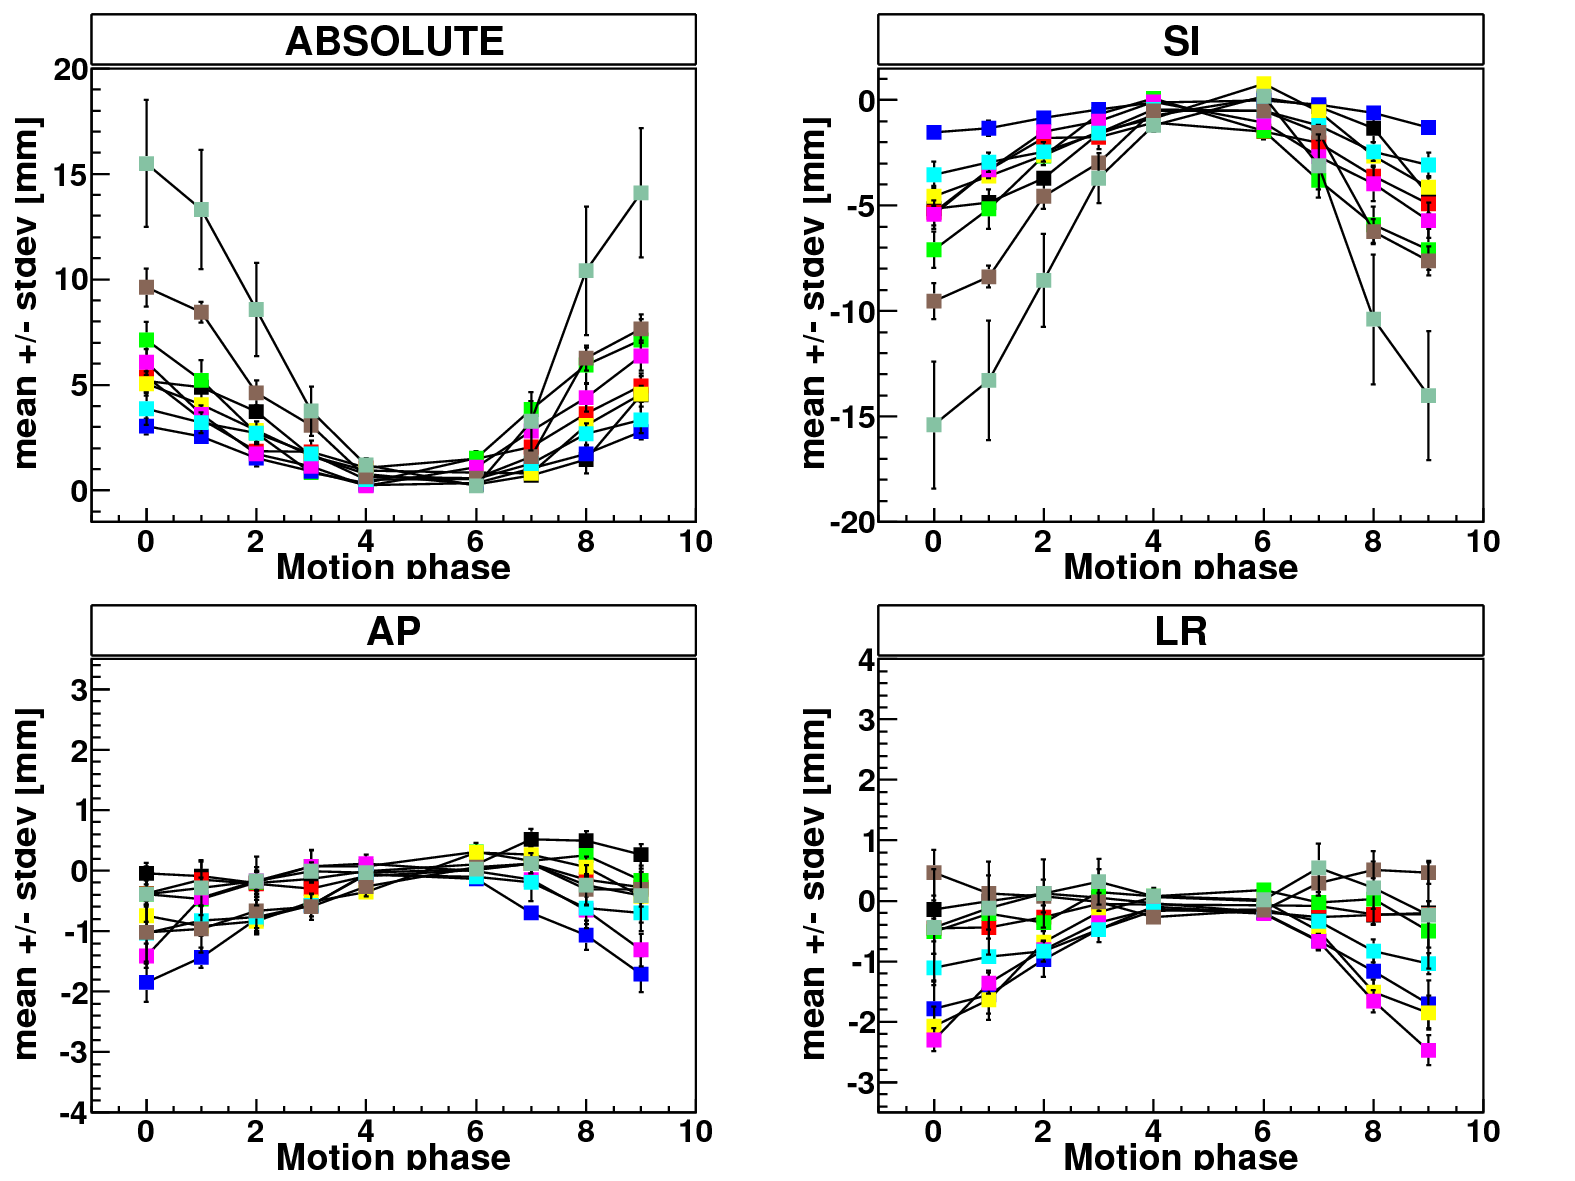
\includegraphics[scale=0.25]{MDACC_allPatients_RESP_LPV.png}
\caption{Motion amplitude of LPV due to respiration for all patients in all motion directions. (patient 1: black, patient 2: red, 
patient 3: green, patient 4: blue, patient 5: yellow, patient 6: pink, patient 7: turquois, patient 8: brown, patient 9: olive) }
\label{motion_resp_all_lpv}
\end{center}
\end{figure}

\begin{figure}[H]
\begin{center}
 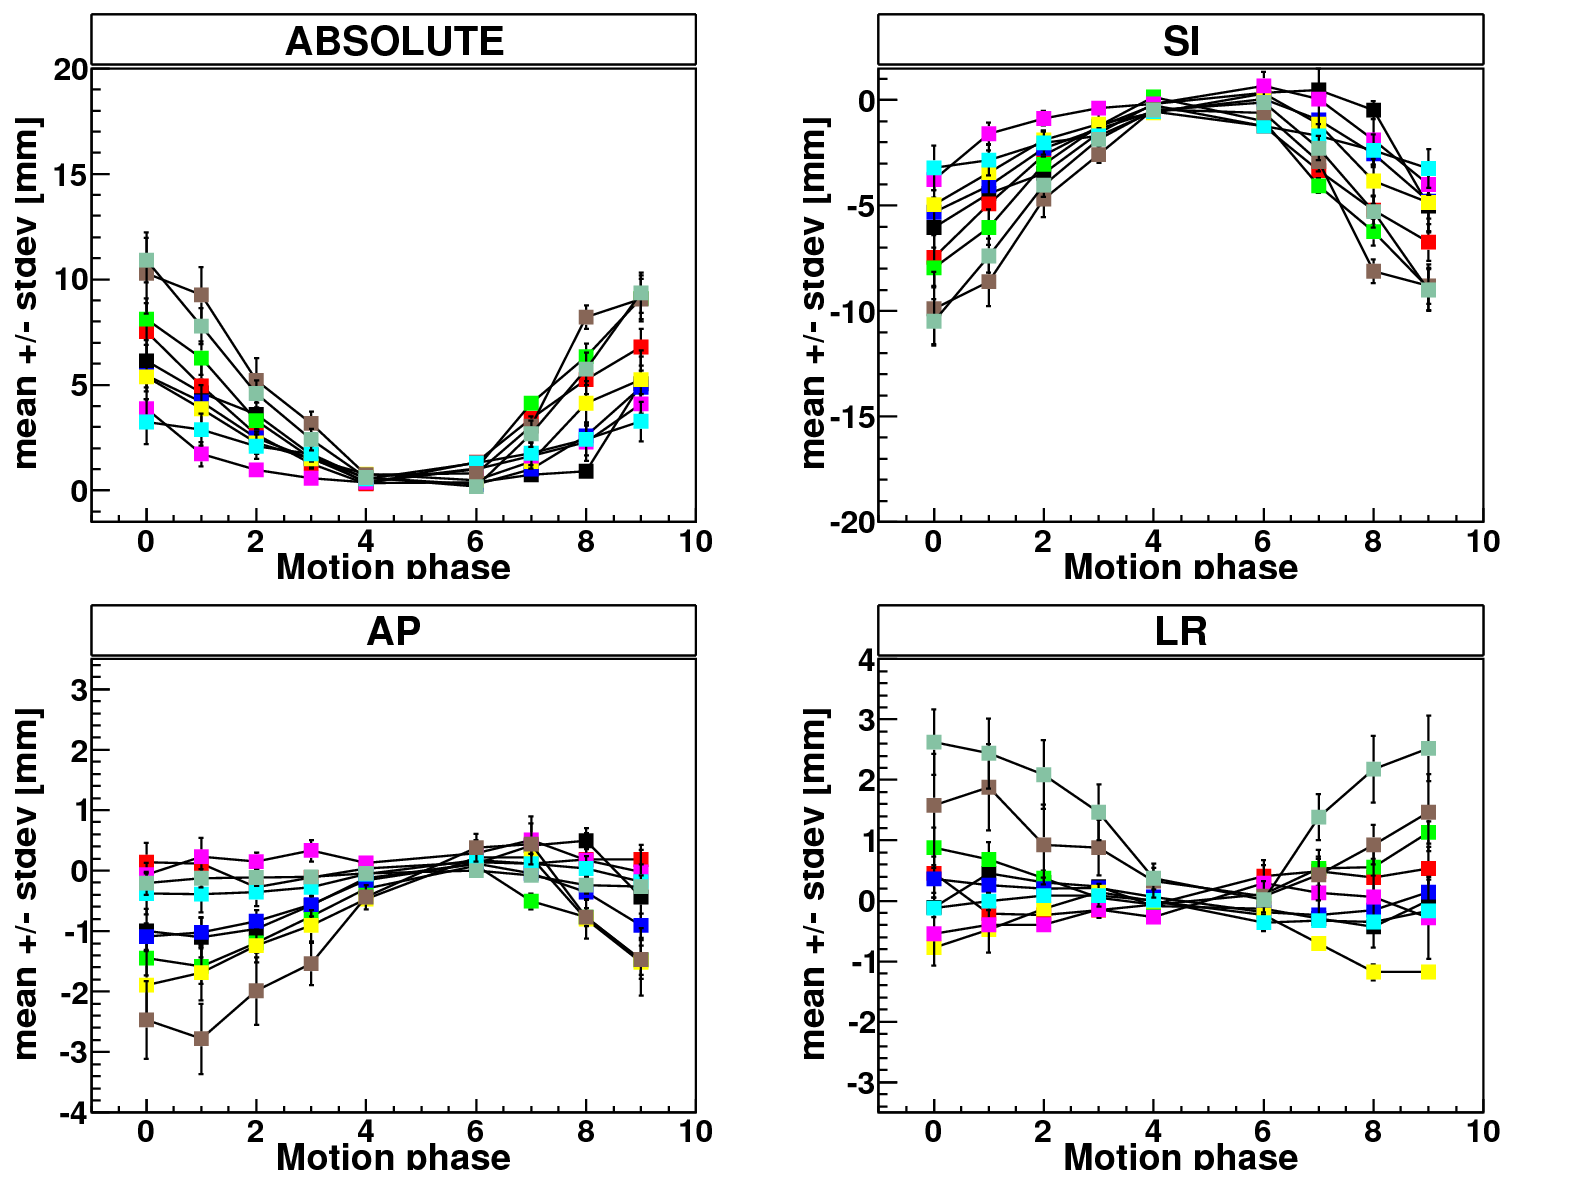
\includegraphics[scale=0.25]{MDACC_allPatients_RESP_RPV.png}
\caption{Motion amplitude of RPV due to respiration for all patients in all motion directions. (patient 1: black, patient 2: red, 
patient 3: green, patient 4: blue, patient 5: yellow, patient 6: pink, patient 7: turquois, patient 8: brown, patient 9: olive) }
\label{motion_resp_all_rpv}
\end{center}
\end{figure}

\vspace*{-0.8cm}

The relative displacement around end exhale (reference phase; motion phase five) is small for all motion directions 
and patients. The displacement relative to the reference phase is highest around motion phases zero at end inhale. \newline 
% The motion in SI direction is higher than in the other two directions (AP and LR).\newline  
\newline
The mean and standard deviation of the displacement between end exhale and end inhale for the different motion directions 
are shown as numerical values in table \ref{tab:motion:LPV} and \ref{tab:motion:RPV} for LPV and RPV, respectively.
Depending on the patient the absolute displacement of the pulmonary veins were found to vary between three millimeters and more than 
one centimeter. The largest motion direction is SI, resulting in the largest contribution to the absolute displacement. The 
average in SI direction over the entire volume reaches up to 15.5mm (average of (6.76 $\pm$ 3.8)mm) for LPV and 10.9mm 
(average of (6.76 $\pm$ 2.5)mm) for RPV. The other two motion directions show a much smaller displacement. In AP direction the maximal 
motion is less than 2.5mm (standard deviation of less than 1mm) and in LR the PVs move less than 2.7mm (standard deviation of 1mm).\newline
\newline
Over all patients, the mean absolute displacement in-between end exhale and end inhale of the LPV is (6.8 $\pm$ 3.6)mm and 
(6.8 $\pm$ 2.5)mm for RPV. For the SI direction, the mean displacement over all patients is (-6.4 $\pm$ 3.8)mm and (-6.6 $\pm$ 2.4)mm for 
RPV.
\newpage

% In AP and LR direction the motion is much smaller. The mean displacement 
% over all patients in AP is (-0.81 $\pm$ 0.54)mm for LPV and (-0.94 $\pm$ 0.84)mm for RPV. For LR it is found to (-0.93 $\pm$ 0.89)mm for 
% LPV and (0.48 $\pm$ 1.02)mm for RPV.\newline

\begin{table}[htbp]
  \centering
  \caption{LPV: Mean and standard deviation of target motion in-between end exhale (motion phase five) and inhale (motion phase zero) for 
  all investigated patients.}
  \begin{tabular}{|c|c|c|c|c|}
    \hline\hline
    patient no\rule{0pt}{2.6ex}\rule[-1.2ex]{0pt}{0pt} & ABS [mm] & SI [mm] & AP [mm] & LR [mm]\\
    \hline
    1 & 5.17 $\pm$ 0.48 & -5.16 $\pm$ 0.48 & -0.05 $\pm$ 0.18 & -0.14 $\pm$ 0.15 \\
    2 & 5.37 $\pm$ 0.62 & -5.33 $\pm$ 0.62 & -0.38 $\pm$ 0.22 & -0.45 $\pm$ 0.22 \\
    3 & 7.14 $\pm$ 0.85 & -7.09 $\pm$ 0.85 & -0.39 $\pm$ 0.40 & -0.51 $\pm$ 0.37 \\
    4 & 3.03 $\pm$ 0.39 & -1.53 $\pm$ 0.26 & -1.85 $\pm$ 0.32 & -1.78 $\pm$ 0.47 \\
    5 & 5.06 $\pm$ 0.57 & -4.55 $\pm$ 0.48 & -0.75 $\pm$ 0.19 & -2.07 $\pm$ 0.32 \\
    6 & 6.08 $\pm$ 0.61 & -5.43 $\pm$ 0.68 & -1.41 $\pm$ 0.20 & -2.30 $\pm$ 0.19 \\
    7 & 3.87 $\pm$ 0.75 & -3.55 $\pm$ 0.63 & -1.03 $\pm$ 0.47 & -1.11 $\pm$ 0.23 \\
    8 & 9.61 $\pm$ 0.90 & -9.53 $\pm$ 0.86 & -1.02 $\pm$ 0.52 & 0.47 $\pm$ 0.38 \\
    9 & 15.50 $\pm$ 3.02 & -15.40 $\pm$ 3.01 & -0.39 $\pm$ 0.46 & -0.44 $\pm$ 0.96 \\
    \hline\hline
  \end{tabular}
  \label{tab:motion:LPV}
\end{table}

\vspace*{-0.5cm}

\begin{table}[htbp]
  \centering
  \caption{RPV: Mean and standard deviation of target motion in-between end exhale (motion phase five) and inhale (motion phase zero) for all 
  investigated patients.}
  \begin{tabular}{|c|c|c|c|c|}
    \hline\hline
    patient no\rule{0pt}{2.6ex}\rule[-1.2ex]{0pt}{0pt} & ABS [mm] & SI [mm] & AP [mm] & LR [mm]\\
    \hline
    1 & 6.12 $\pm$ 1.43 & -6.03 $\pm$ 1.41 & -1.00 $\pm$ 0.37 & -0.11 $\pm$ 0.16 \\
    2 & 7.51 $\pm$ 1.35 & -7.47 $\pm$ 1.35 & 0.14 $\pm$ 0.32 & 0.46 $\pm$ 0.41 \\
    3 & 8.12 $\pm$ 0.98 & -7.94 $\pm$ 0.95 & -1.45 $\pm$ 0.28 & 0.88 $\pm$ 0.33 \\
    4 & 5.46 $\pm$ 0.57 & -5.33 $\pm$ 0.59 & -1.09 $\pm$ 0.22 & 0.36 $\pm$ 0.23 \\
    5 & 5.37 $\pm$ 1.51 & -4.96 $\pm$ 1.44 & -1.89 $\pm$ 0.56 & -0.77 $\pm$ 0.12 \\
    6 & 3.85 $\pm$ 0.46 & -3.77 $\pm$ 0.48 & -0.07 $\pm$ 0.20 & -0.55 $\pm$ 0.52 \\
    7 & 3.25 $\pm$ 1.08 & -3.21 $\pm$ 1.06 & -0.38 $\pm$ 0.34 & -0.12 $\pm$ 0.10 \\
    8 & 10.30 $\pm$ 1.91 & -9.89 $\pm$ 1.74 & -2.47 $\pm$ 0.64 & 1.58 $\pm$ 0.85 \\
    9 & 10.90 $\pm$ 1.06 & -10.50 $\pm$ 1.06 & -0.21 $\pm$ 0.19 & 2.62 $\pm$ 0.54 \\
    \hline\hline
  \end{tabular}
  \label{tab:motion:RPV}
\end{table}

% \vspace*{-0.2cm}

% It can be stated that the underlying respiration amplitude (see table \ref{tab:patdata}) does not strongly correlate with the absolute 
% motion amplitude of the PVs. While patient 6 and 7, who have a motion amplitude of 2.5mm and 5mm, respectively, were also found to have the 
% smallest absolute displacement in case of RPV, the smallest absolute motion of LPV were found in patient 4, who displays a rather big respiration 
% amplitude of 17.5mm. The biggest displacement on the other hand was found in patient 8 and 9, who also display the biggest respiration amplitude. 
% Nevertheless, the maximal absolute displacement was found in the LPV to (15.50 $\pm$ 3.02)mm and in RPV to (10.90 $\pm$ 1.06) (both in 
% patient 9), who only has the second biggest respiration amplitude after patient 8.\newline

\vspace*{0.5cm}

Possible correlations between the underlying respiration amplitude (see table \ref{tab:patdata}) and the displacement of the ablation sites 
for the PVs have been studied (see figure \ref{corr_motion}). It can be stated that in AP and LR direction, no correlation was 
observed. In case of SI displacement the results varied depending on the target volume. While no correlation was 
observed between the SI displacement and the diaphragm motion in the ablation site of the LPV, the site for RPV showed a strong linear 
relationship (r=0.79, p<0.05). This resulted in a strong correlation between absolute diaphragm motion and RPV ablation site (r=0.79, p<0.05). 
For the LPV again no correlation was observed in the absolute displacement. \newline
\newline
It should be noted that these findings are based on lung cancer 
patients (see table \ref{tab:patdata}), which can alter the breathing pattern and heart motion and hence the result. It is unclear whether 
atrial fibrillation patients would display the same motion dependence and correlation results, though the result was independent of 
the tumor position in the left or right lung. 



%%%% Korrelationen zwischen Diaphragma motion and motion LPV/RPVs
\newpage

\begin{figure}[H]
\centering
\subfigure[LPV: absolute]{
 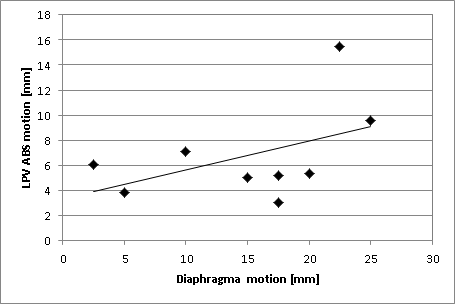
\includegraphics[scale=0.58]{Corr_LPV_ABS.png}
 }
\subfigure[RPV: absolute]{
 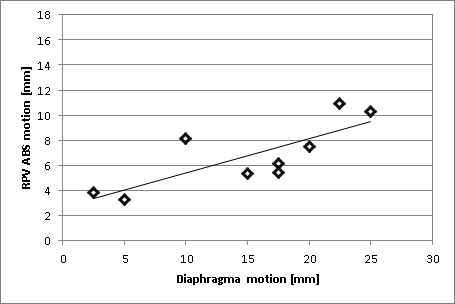
\includegraphics[scale=0.58]{Corr_RPV_ABS.png}
 }
\subfigure[LPV: SI]{
 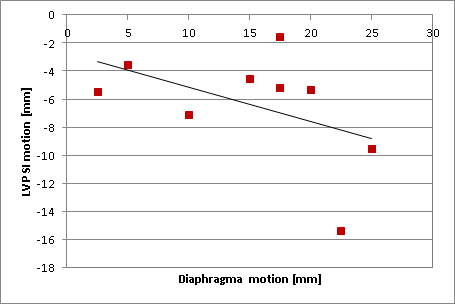
\includegraphics[scale=0.58]{Corr_LPV_SI.png}
 }
\subfigure[RPV: SI]{
 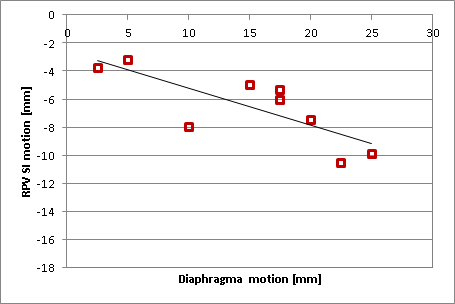
\includegraphics[scale=0.58]{Corr_RPV_SI.png}
 }
\subfigure[LPV: AP]{
 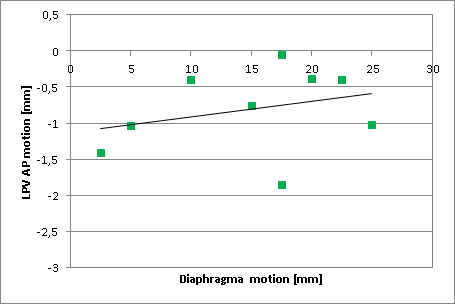
\includegraphics[scale=0.58]{Corr_LPV_AP.png}
 }
\subfigure[RPV: AP]{
 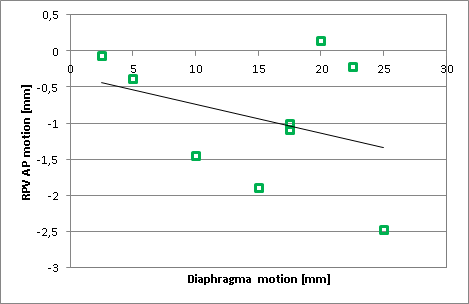
\includegraphics[scale=0.58]{Corr_RPV_AP.png}
 }
\subfigure[LPV: LR]{
 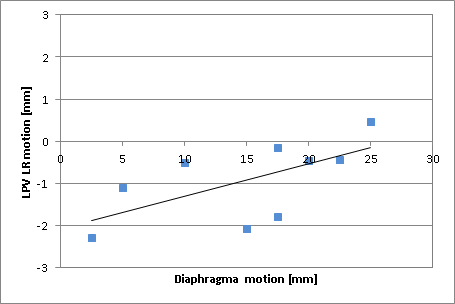
\includegraphics[scale=0.58]{Corr_LPV_LR.png}
 }
\subfigure[RPV: LR]{
 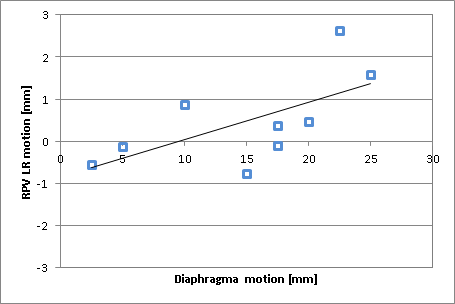
\includegraphics[scale=0.58]{Corr_RPV_LR.png}
 }
\caption{Motion of the ablation site of LPV (left column) and RPV (right column) in relation to the diaphragmatic motion of the respective patient. 
The motion is plotted as mean value of: absolute displacement, SI displacement, AP displacement and LR displacement, respectively.}
\label{corr_motion}
\end{figure}

\newpage

The overall displacement field between the two extreme states, end exhale and end inhale, for two exemplary patients with a small motion 
amplitude (patient 7) and a large motion amplitude (patient 9) are shown in figure \ref{contour_pat036} and \ref{contour_pat122}. In order to 
visualize the location of the displacement, an axial cut of the reference state CT is underlayed. The absolute values of the displacement 
vectors are shown as contour plots. 

\begin{figure}[H]
\begin{center}
 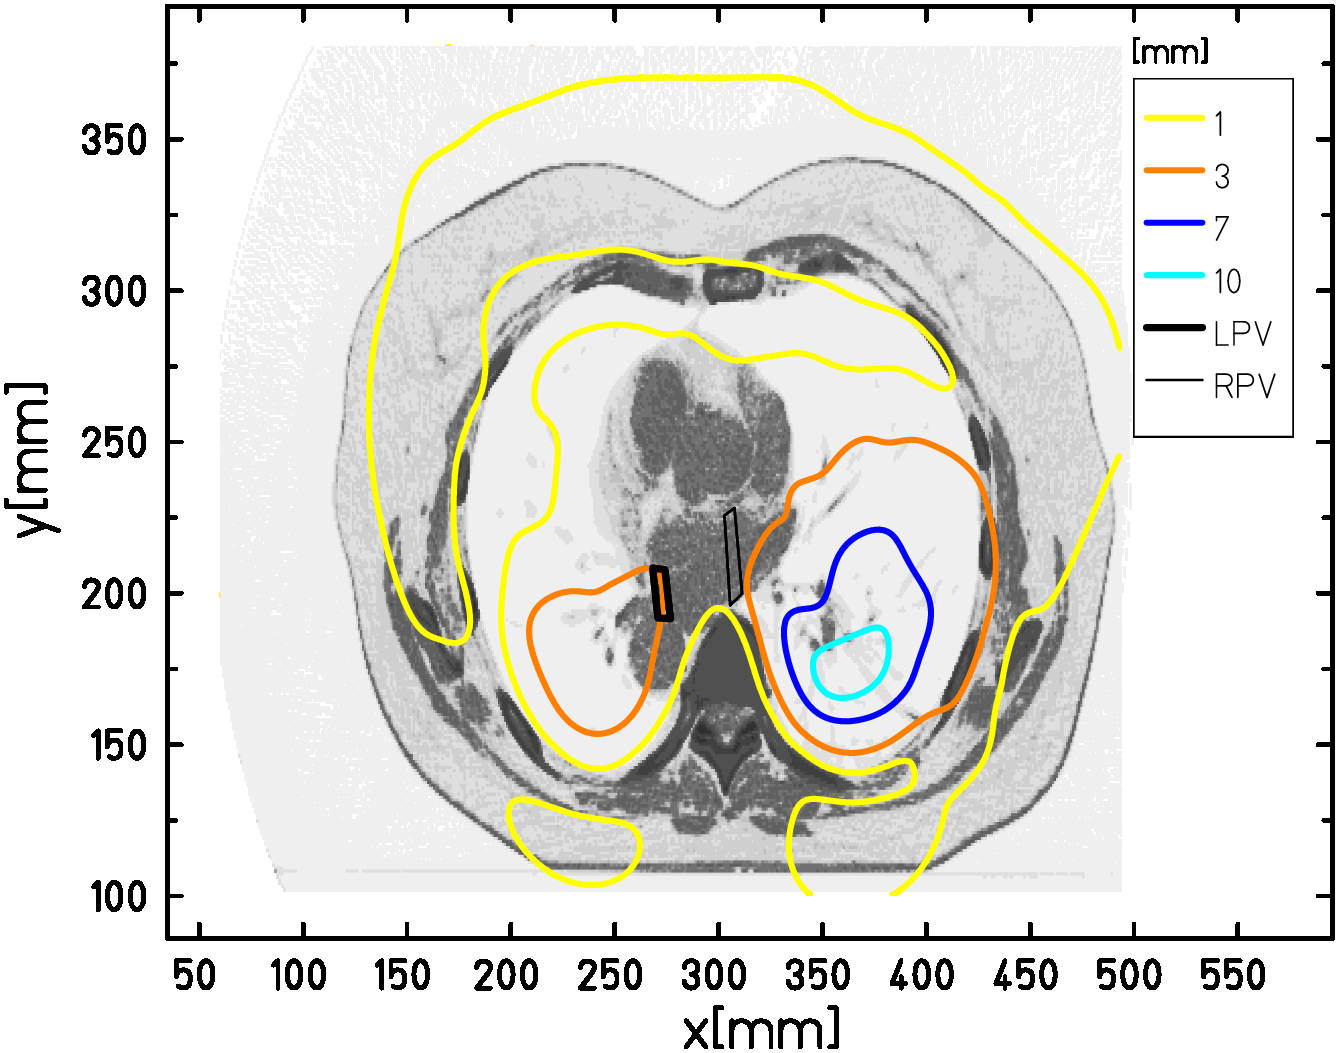
\includegraphics[scale=0.22]{Contour_z_abs_RESP_Pat037_gedreht.png}
\caption{Contour plot of Patient 7}
\label{contour_pat036}
\end{center}
\end{figure}

\begin{figure}[H]
\begin{center}
 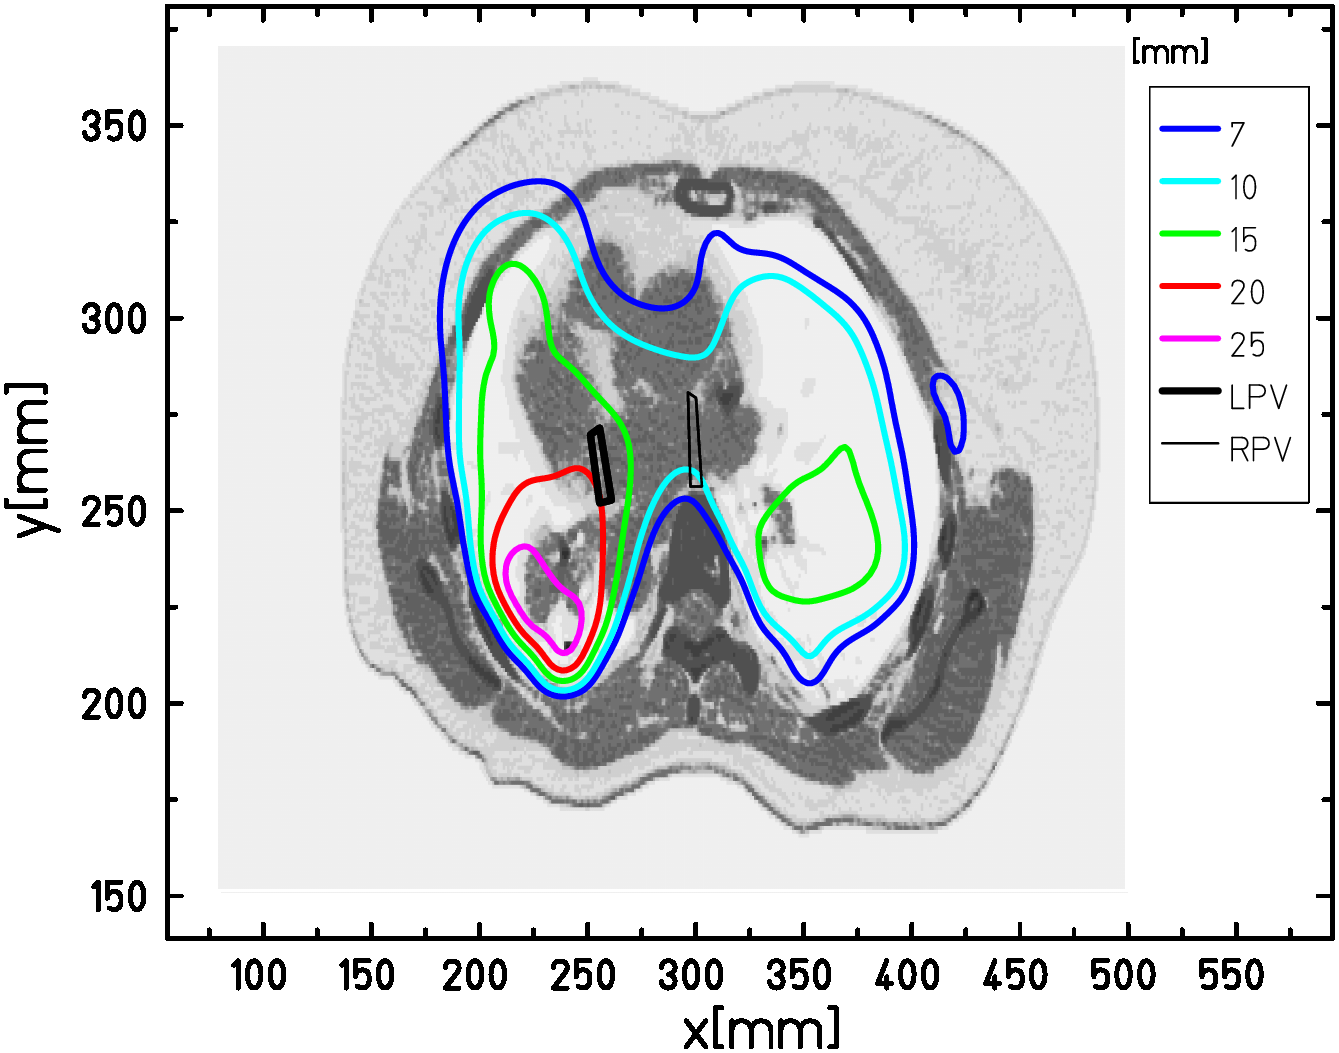
\includegraphics[scale=0.22]{Contour_z_abs_RESP_Pat122_gedreht.png}
\caption{Contour plot of Patient 9 }
\label{contour_pat122}
\end{center}
\end{figure}

\newpage



% - motion LPV > motion RPV
% - Pat122 and Pat039 largest motion both in LPV and RPV
% - smallest motion: LPV: 031, RPV: 036
% - MP 4, 5, 6 smallest motion -> gating
% - biggest motion in SI, LR and AP rather small
% 
% (- motion je patient fuer LPV und RPV in anhang ?)


%%%%%%%%%%%%%%%%%%%%%%%%%%%%%%%%%%%%%%%%%


\subsection{Motion mitigation techniques for respiration}
\label{mmt}
The absolute motion amplitudes of up to 1cm due to respiration are expected to yield dose inhomogeneity when not compensated for. The 
resulting Interplay effect and dose deposition was studied for every patient for different motion patterns and different margins to the target 
volumes. The dose analysis values V95, V107 and D5-D95 were assessed and plotted. For comparison also the corresponding 
values for the 3D case (static) are shown. As shown in section \ref{motion} the motion displacement in the motion phases around 
end exhale (motion phase four to motion phase six) are rather small in all patient cases. Hence gating has the potential to be a 
well-suited motion mitigation technique to overcome the influence of target volume motion due to respiration. The results of the stated dose 
values in case of gating on the stated phases will also be presented. 


\subsubsection{Dose deposition}

A representative dose deposition for all studied techniques (static, interplay and gating) is shown exemplary for patient 9 (as this is the 
patient with the largest PV motion amplitude) in figure \ref{dose_pat122}. Gating and interplay are shown for a motion with a period of 6 s 
and a starting phase of 0$^{\circ}$. The target volumes LPV and RPV were irradiated simultaneously and a margin of 3mm was added. It can 
already been seen from this dose cut figures that gating around end expiration drastically improves the outcome compared to interplay and yields 
a result which is comparable to the static case.\newline
\newline
In order to assess the dose information for the whole volume the DVHs of all patients were analyzed and compared for dose steepness, 
dose coverage as well as over dosage. The average results over all patients with the resulting standard deviation can be seen in 
figure \ref{static_interplay_gating}. A more detailed analysis can be found in appendix XXX, where the values are plotted for each patient 
(figures \ref{static_interplay_gating_Pat01} - \ref{static_interplay_gating_Pat09}) and all corresponding numerical values are shown.\newline
\newline
For interplay it can be seen that the results are dependent on the used motion period and starting phase, the safety margin and 
the studied patient case. The underlying deformation map with its motion amplitude does not enable a prediction of the magnitude of the 
interplay effect. The correlation between absolute motion amplitude of the left and right PV and the resulting V95 value for 3 mm Margin were
assessed for all studied motion patterns (Lujan motion with period of 6s or 8s and starting phase of 0$^{\circ}$ and 90$^{\circ}$) and patients. 
A correlation between the dose coverage and amplitude resulted in some cases where a motion period of 6s was chosen (LPV: r=0.69 and starting 
phase of 0$^{\circ}$, r=0.86 for starting phase of 90$^{\circ}$; RPV: r=0.73 for starting phase of 90$^{\circ}$; all p<0.05). 
Nevertheless these results could not be verified in the other motion cases and hence no clear dependence between target volume displacement 
and dose coverage was found. Concerning safety margins a tendency towards improved dose homogeneity and coverage can be seen with increasing 
margin. However, a study of the linear correlation between the two values for all the different motion patterns and all patients showed no 
clear dependence.\newline
% The under dosage in the LPV of patient 8, who has one of the largest motion amplitude in the studied cases, is found to be 
% V95 = 96.55\% for a margin of 3mm (and motion period of 6 s, starting phase of 90$^{\circ}$) while having a dose steepness of 
% D5-D95 = 9\%. Patient 6 on the other hand, who has one of the smallest studied motion amplitude, has a very comparable result for the same 
% safety margin and motion case with V95 = 96.60\% and D5-D95 = 8\%. In general the values tend to improve for interplay with increasing margin. Nevertheless in 
% some cases a smaller safety margin of 3mm leads to an improved reduction of under dosage compared to 5mm or 7mm margin (e.g. patient 6, LPV, 
% Lujan with motion period 8 s and motion starting phase of 0$^{\circ}$: V95 = 93.41\% for 3mm Margin, V95 = 90.37\% for 5mm Margin and V95 = 
% 92.77\% for 7mm Margin).\newline
\newline
Gating yielded improved results compared to interplay in all studied cases. This is valid for dose steepness, dose coverage as 
well as over dosage. Especially dose coverage and over dosage are comparable to the static results for all patient and motion patterns 
(e.g. patient 1, V95 of 100\% for all studied motion patterns and safety margins in RPV). In some patients the dose coverage is better  
with added safety margins (e.g. patient 9, V95 with no margin for motion period of 6 s and starting phase of 0$^{\circ}$ is 94.14 \% for LPV, 
a V95 of 99.92 \% can be achieved for the same motion pattern with a margin of 3mm). Also in dose steepness a bigger safety margin tends to 
improve results (e.g. in LPV of patient 6 with motion period of 8 s with starting phase of 90$^{\circ}$: D5-D95 = 4.63\% with margin of 3mm 
versus D5-D95 = 4.21 \% with margin of 5mm). Nevertheless a linear correlation between safety margin and 
dose coverage value as well as dose homogeneity has not been found in all patients and all motion pattern. 
Dose steepness is the only value which can not be drastically improved by gating compared to interplay in all cases. Patient 2 for example 
has a D5-D95 value of 6.79\% for gating with a safety margin of 3mm (motion with period of 6 s and starting phase of 90$^{\circ}$), which is 
only slightly under the interplay result of D5-D95=8.41\% for the same safety margin and motion. Nevertheless the dose steepness value of 
interplay in this particular patient case is already lower than in other cases (e.g. patient 1, LPV: D5-D95=10.60\% for a safety margin of 3mm 
and a motion with a period of 6 s and a starting phase of 90$^{\circ}$; patient 9, LPV: D5-D95=20.93\% for a safety margin of 3mm and a motion 
with a period of 6 s and a starting phase of 90$^{\circ}$).\newline
\newline
A method to further improve the dose steepness can be rescanning in the gating window. This has been studied for two patient cases 
and the results are shown in the next section (Rescanning of gated volume).
\newline
% It can be concluded that gating yields improved dose coverage (under and over dosage) and better dose steepnesses compared to interplay in 
% all studied patient cases, motion patterns and for all safety margins. It can thus be an adequate motion mitigation technique for the 
% irradiation of PVs under influence of respiratory motion. 



% - folgende ergebnisse geordnet nach kleiner bewegung, mittlerer bewegung und grosser bewegung
% - V95 and V107 ok; D5-D05 fuer gating koennte besser sein. hier +rescan ? conformity index statt dessen?
% - dy dose cut to illustrate dose homogeneity?
% 
% - obwohl motion lpv > rpv ist interplay in rpv schlimmer (fuer Pat023), bei 023 vll auch motion rpv > lpv. wuerde sinn machen

% - XXX values in tabelle fuer appendix 



\newpage

 \begin{figure}[H]
 \begin{center}
\subfigure[static]{
 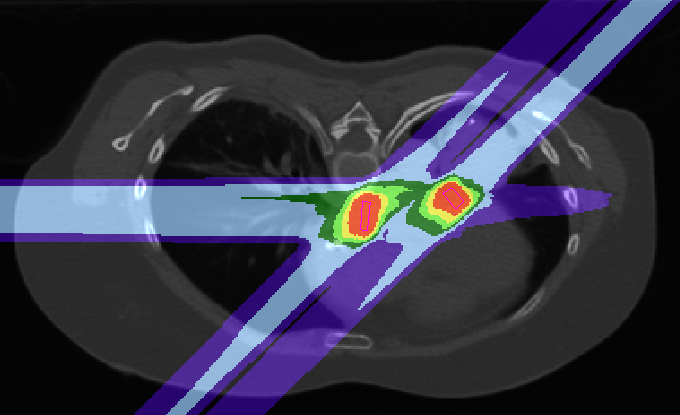
\includegraphics[scale=0.6, angle=180]{Pat122_slice48_static.png}
 }
\subfigure[interplay]{
 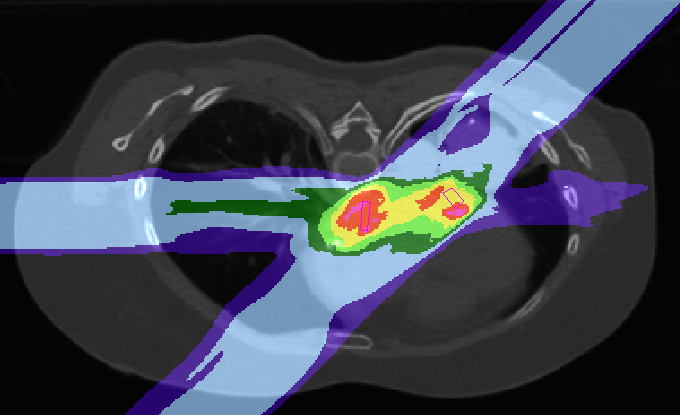
\includegraphics[scale=0.6, angle=180]{Pat122_slice48_interplay.png}
 }
 \subfigure[gating]{
 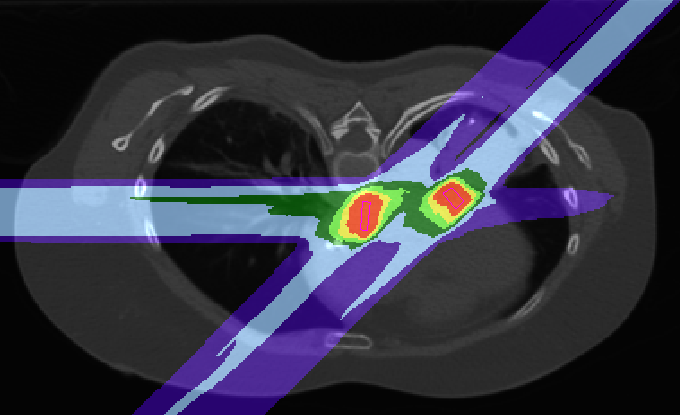
\includegraphics[scale=0.6, angle=180]{Pat122_slice48_gating.png}
 }
\caption{Dose distribution of patient 9 for static (a) as well as interplay (b) and gating (c) at motion period of 6 s and a motion starting 
phase of 0$^{\circ}$. The target volume has an added margin of 3mm. The improved outcome of gating compared to interplay 
can already be seen in these dose cuts.}
\label{dose_pat122}
 \end{center}
\end{figure}

\newpage

\begin{figure}[H]
\subfigure[D5-D95: LPV]{
 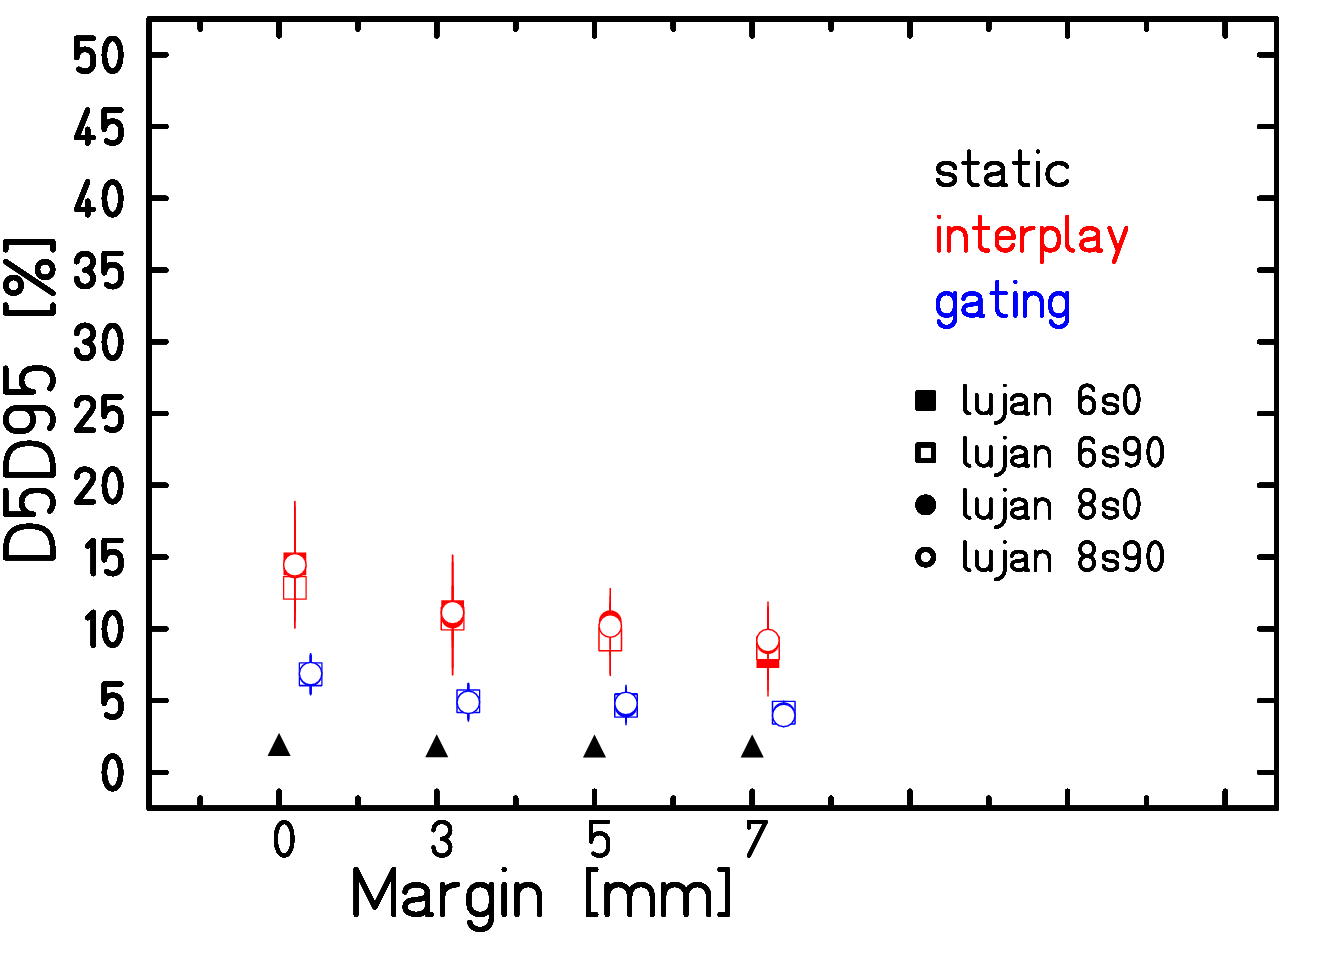
\includegraphics[scale=0.18]{MDACC_CTV_LPV_D5D95.png}
 }
 \subfigure[D5-D95: RPV]{
 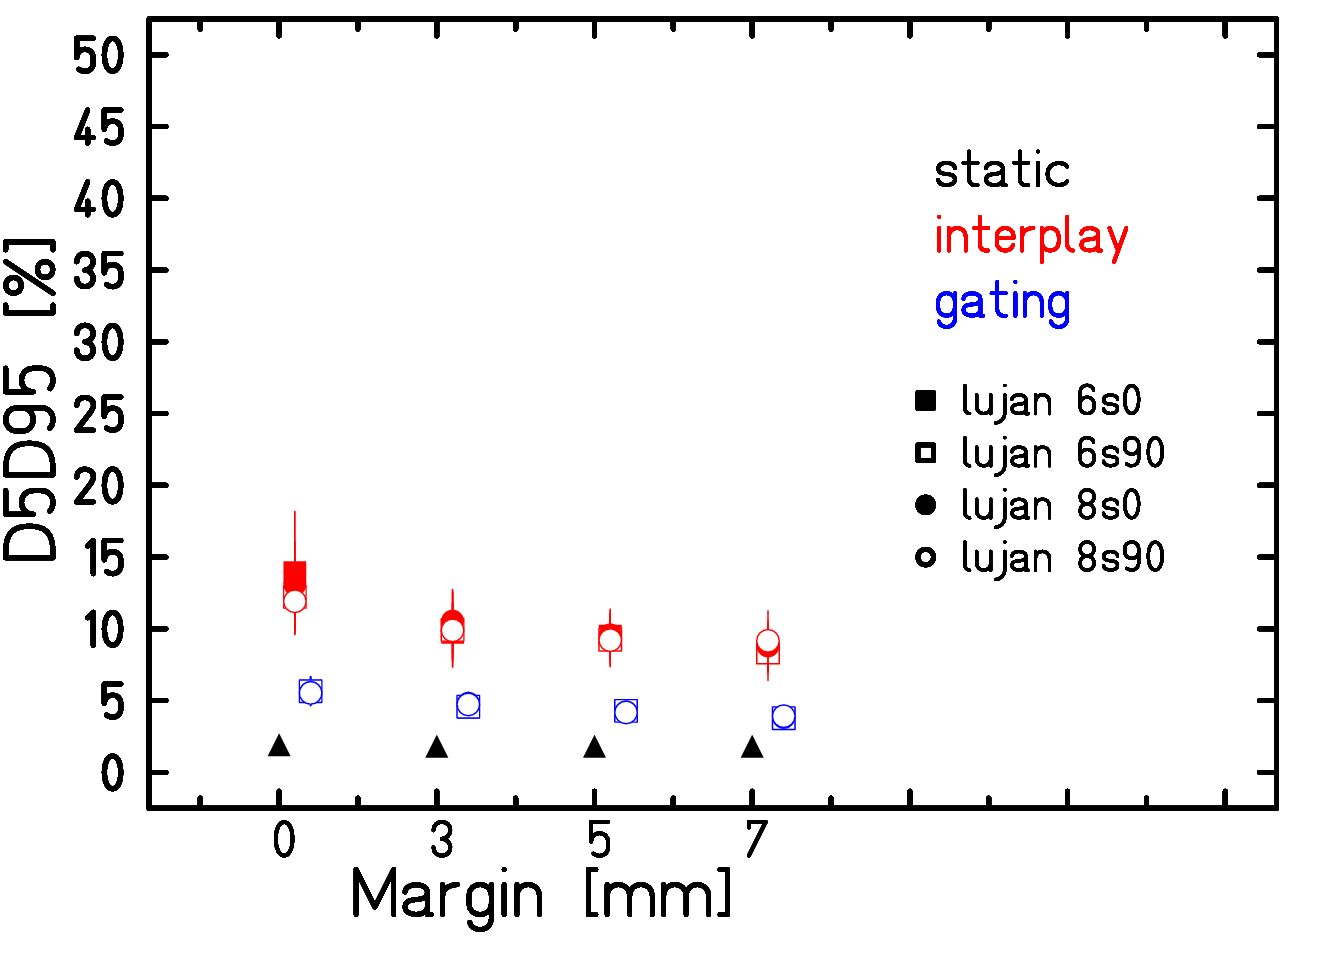
\includegraphics[scale=0.18]{MDACC_CTV_RPV_D5D95.png}
 }
 \subfigure[V95: LPV]{
 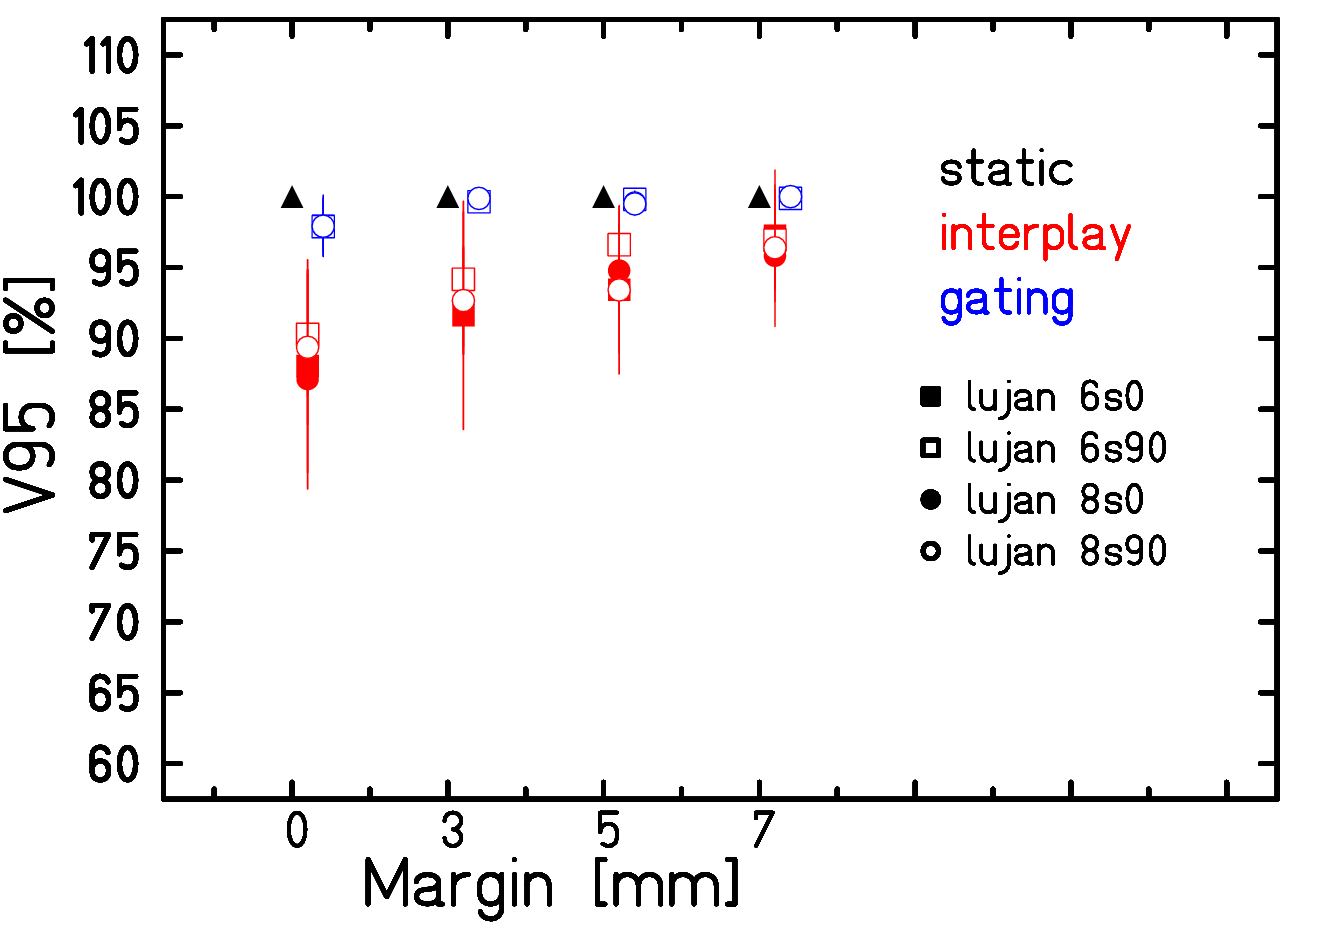
\includegraphics[scale=0.18]{MDACC_CTV_LPV_V95.png}
 }
\subfigure[V95: RPV]{
 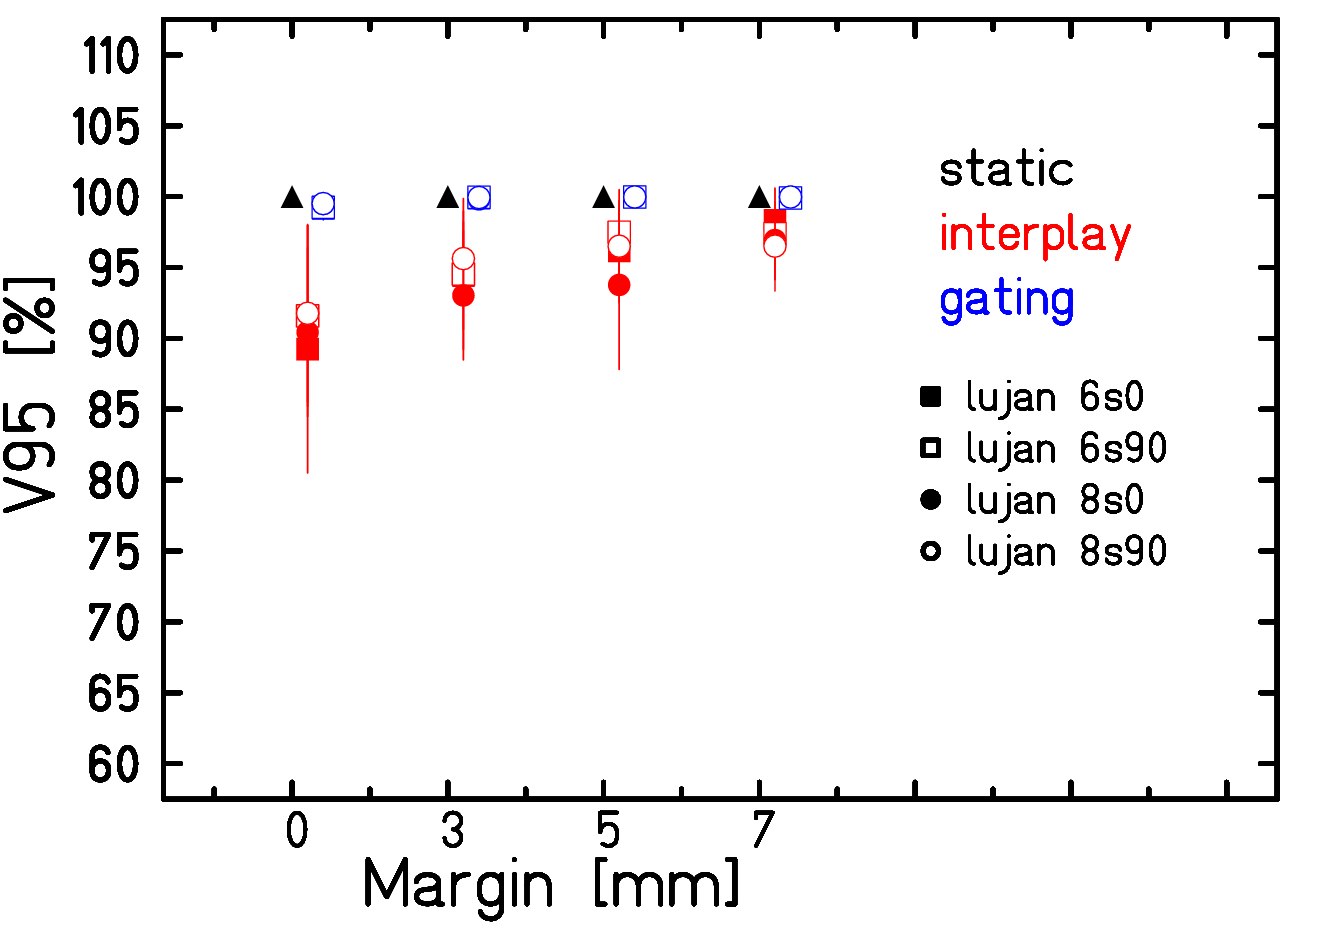
\includegraphics[scale=0.18]{MDACC_CTV_RPV_V95.png}
 }
  \subfigure[V107: LPV]{
 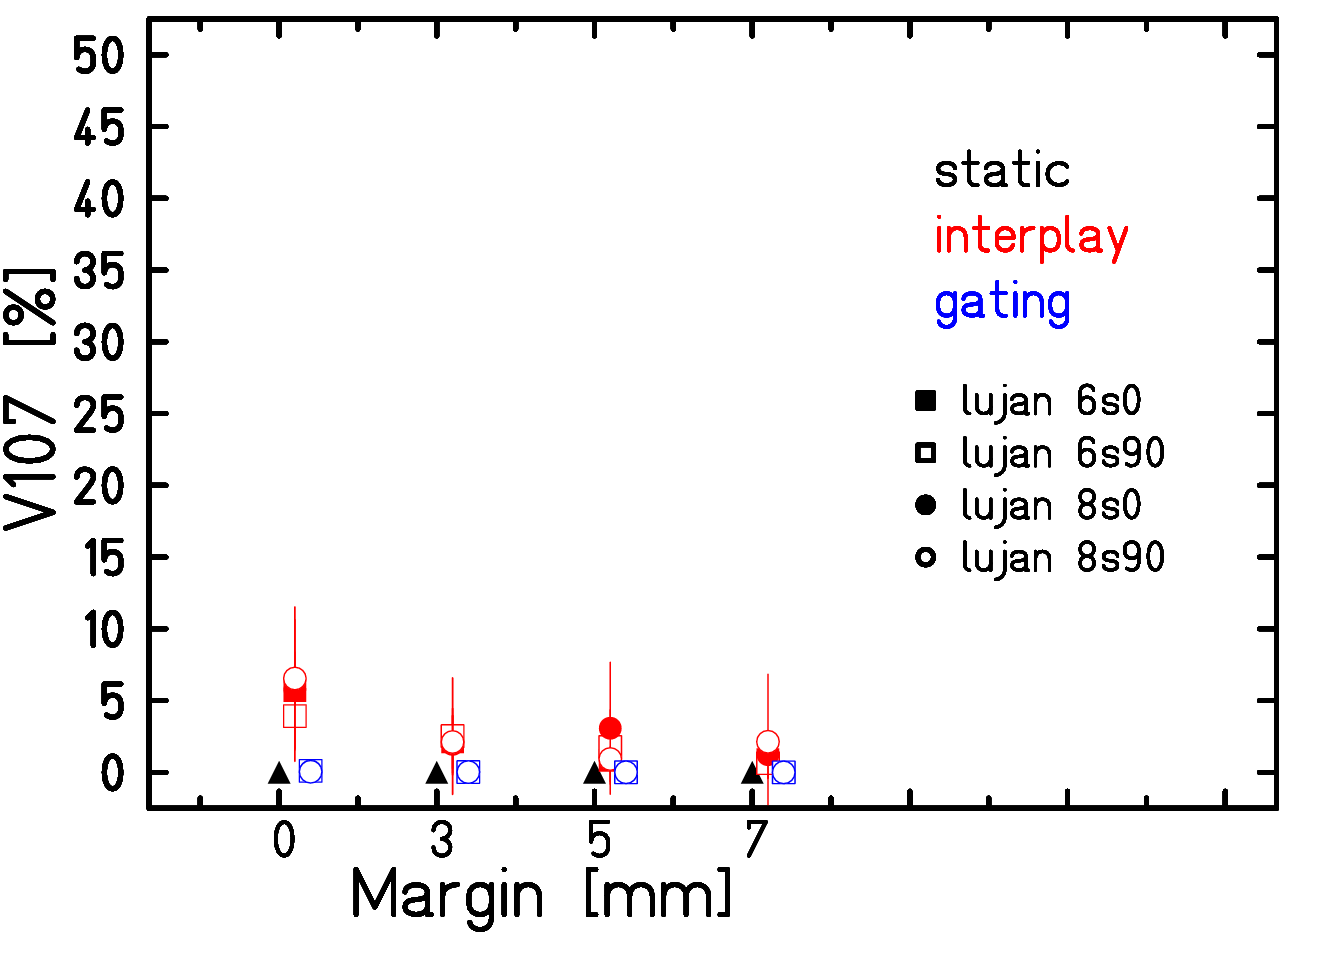
\includegraphics[scale=0.18]{MDACC_CTV_LPV_V107.png}
 }
\subfigure[V107: RPV]{
 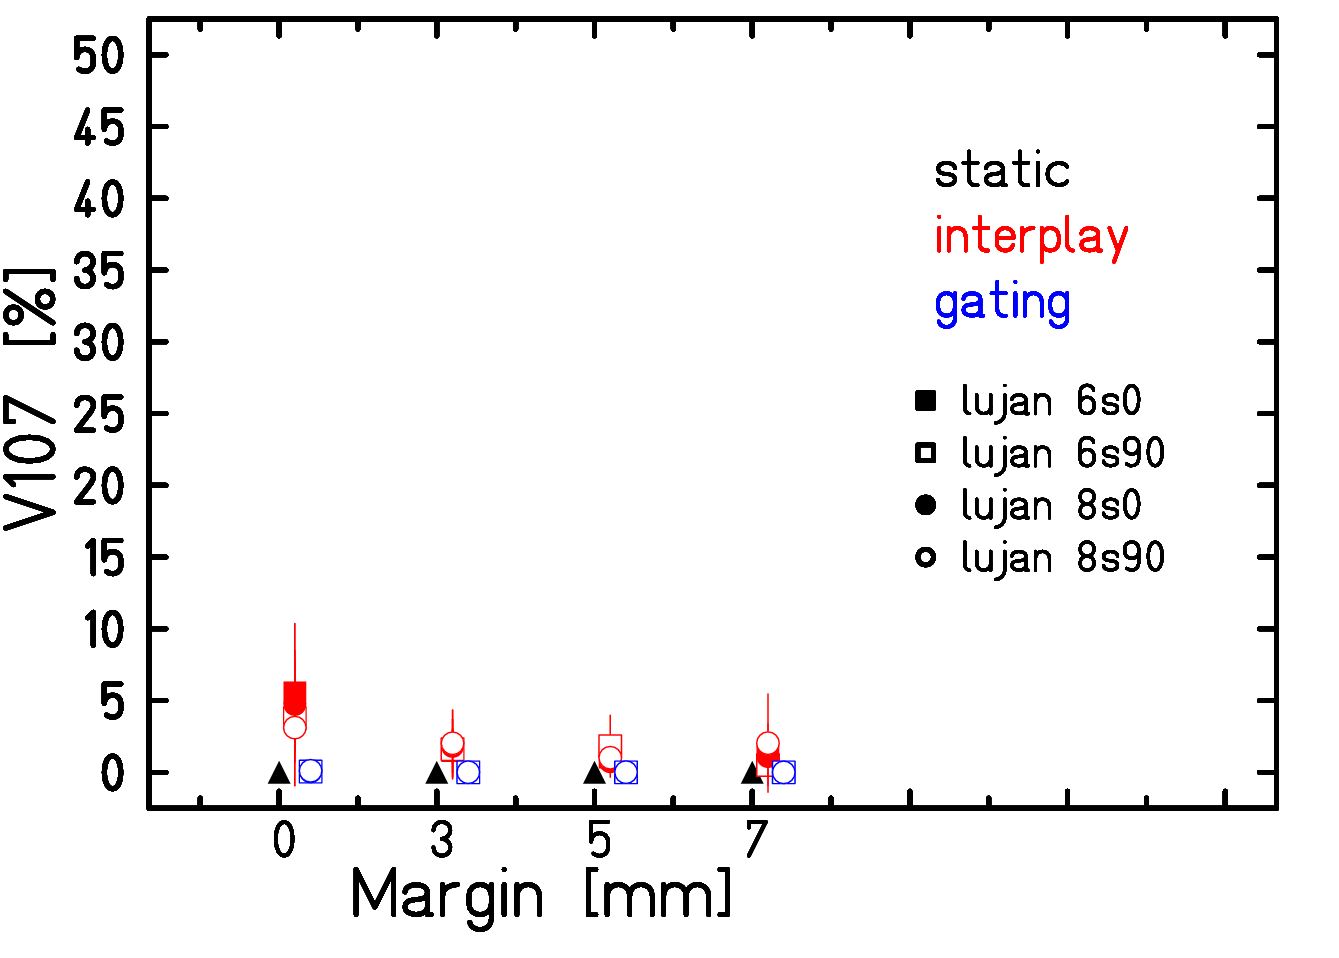
\includegraphics[scale=0.18]{MDACC_CTV_RPV_V107.png}
 }
\caption{Mean value and standard deviation of dose analysis parameters D5-D95 (dose homogeneity, first row), V95 (dose coverage, middle row) 
and V107 (over dosage, last row) over all patients. The LPV (left column) and RPV (right column) were studied seperately. Static (black) as well as interplay (red) and gating (blue) 
are compared for four different motions and different safety margins.}
\label{static_interplay_gating}
\end{figure}


\newpage 

\subsubsection*{Rescanning of gated volume}
\label{RescanofGate}

% - rescan: V95 and V107 as static, D5D95 improved (e.g.margin 3mm: 7 to 3 or 4)
% - which rescan number yields sufficient good results? 10?

The combination of two motion mitigation techniques, gating and rescanning, would directly apply when not only the respiratory motion but 
also the heart beat would be compensated for (see chapter XXX). In order to study the outcome of such a delivery, several number of rescans 
(5, 10, 15 and 20) were applied on the gated irradiation for patient 2 (as an example of a patient with a medium absolute displacement of the 
target volumes) and patient 9 (with the highest studied absolute displacement). The results can be seen in figure 
\ref{static_interplay_gating_rescan_Pat02} and \ref{static_interplay_gating_rescan_Pat09}. The numerical results are shown in appendix XXX.\newline
\newline
It becomes obvious that rescanning does further improve the dose delivery, especially regarding dose homogeneity. For patient 2 
dose homogeneity values in LPV of 6.79\% of the prescribed physical dose of 25 Gy with gating (3 mm margin, Lujan motion with 6s period and starting 
phase of 90$^{\circ}$) can be further improved to 4.69\% with only five rescans or 3.95\% with fifteen rescans. In RPV dose homogeneity values of 
4.95\% for the same margin and motion can be improved to 4.78\% with five rescans and 3.82\% with fifteen rescans. 
For patient 9 the dose homogeneity value of 5.01\% for LPV with 3mm margin and Lujan motion period of 6s and starting phase of 90$^{\circ}$ can 
be improved to 3.83\% with only five rescans. For the RPV dose homogeneity of 4.42\% with the same margin and motion results to 
3.94\% with five rescans.\newline
\newline
It can be concluded that especially patients with a large motion amplitude, and hence an increased residual motion inside the gating window, 
can benefit from an overlay of rescanning as a second motion mitigation technique. A small number of rescans, e.g. five, is already 
sufficient to yield an improved dose homogeneity. As not only respiration but also heart beat needs to be compensated for when irradiating 
target volumes in the heart (see chapter XXX), the presented combination of motion mitigation techniques is feasible and adequate. 

\newpage

\begin{figure}[H]
\subfigure[D5-D95: LPV]{
 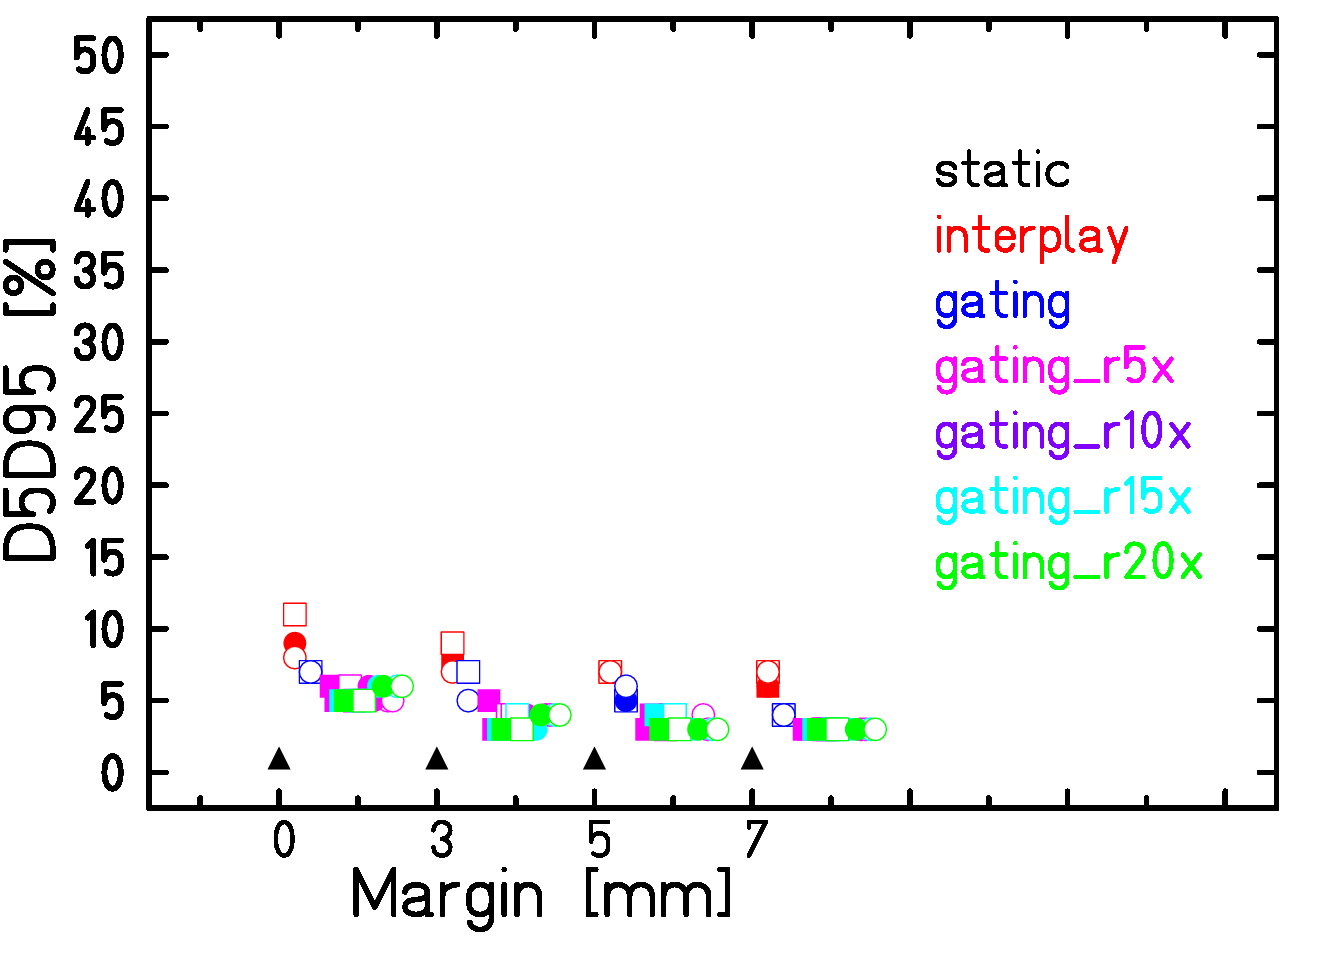
\includegraphics[scale=0.18]{MDACC_Pat024_CTV_LPV_D5D95_withRescan.png}
 }
 \subfigure[D5-D95: RPV]{
 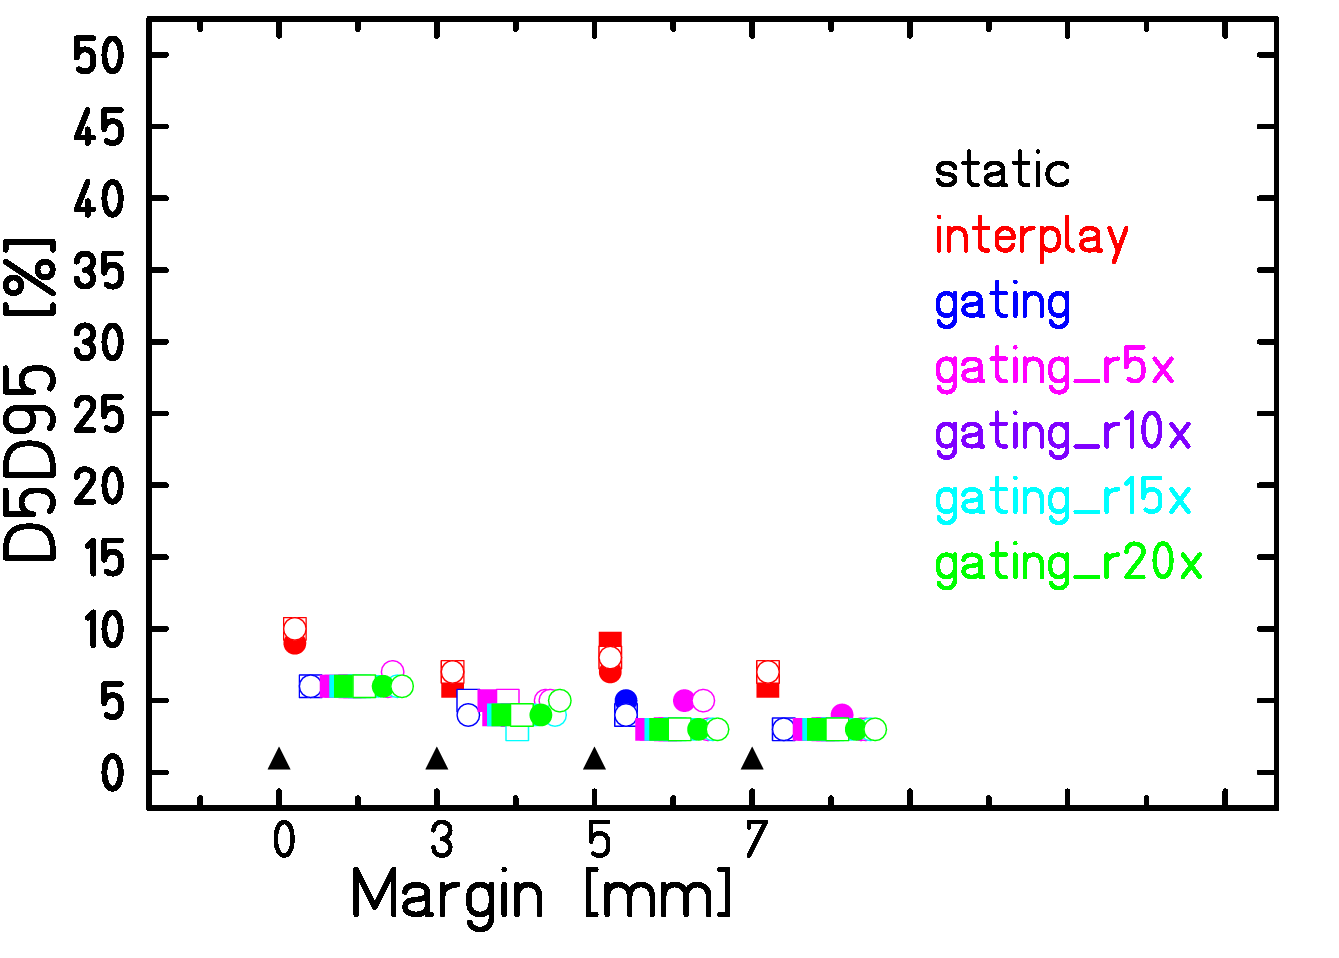
\includegraphics[scale=0.18]{MDACC_Pat024_CTV_RPV_D5D95_withRescan.png}
 }
 \subfigure[V95: LPV]{
 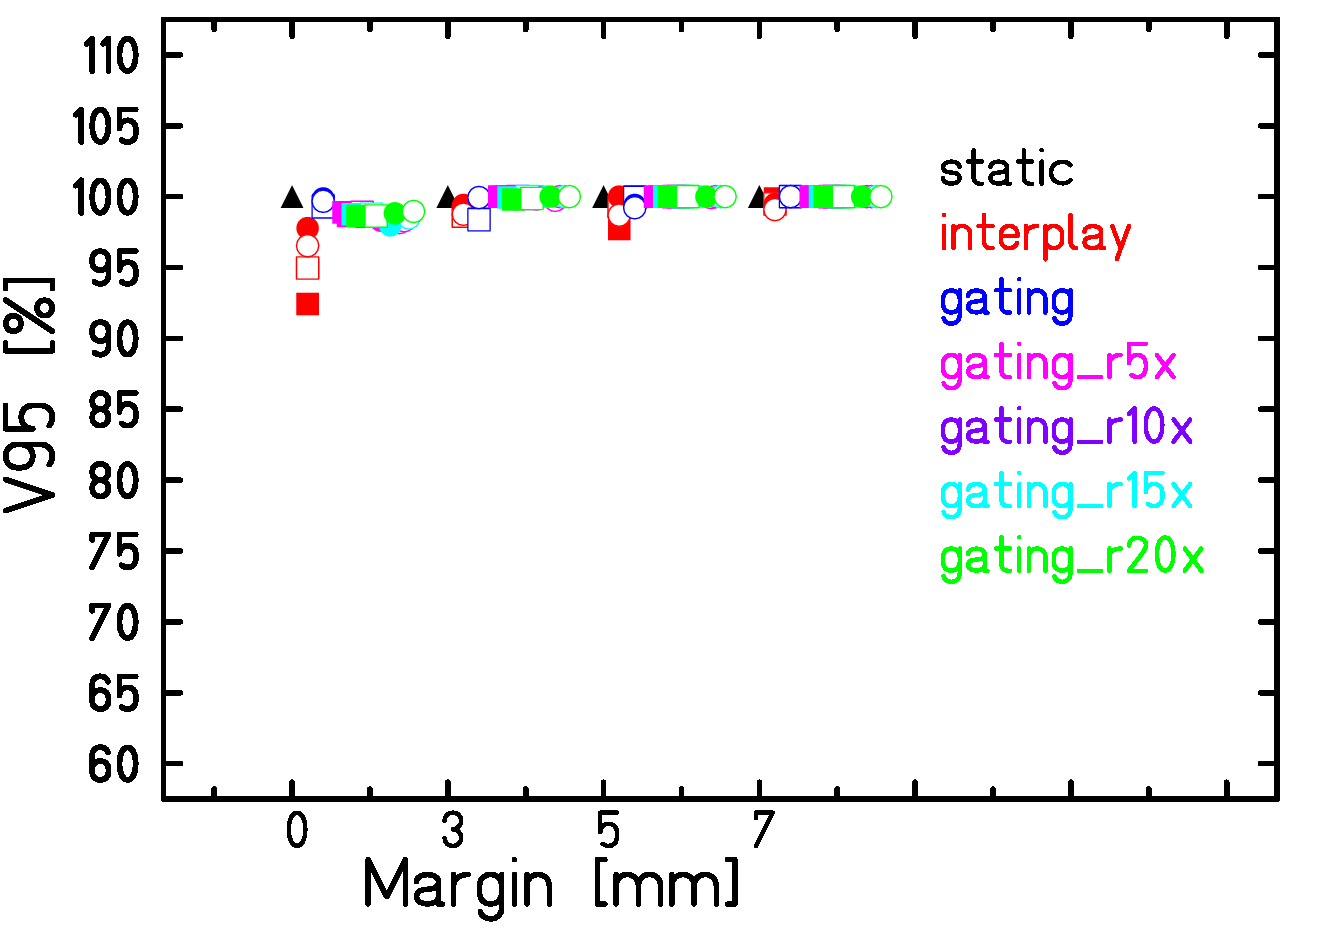
\includegraphics[scale=0.18]{MDACC_Pat024_CTV_LPV_V95_withRescan.png}
 }
\subfigure[V95: RPV]{
 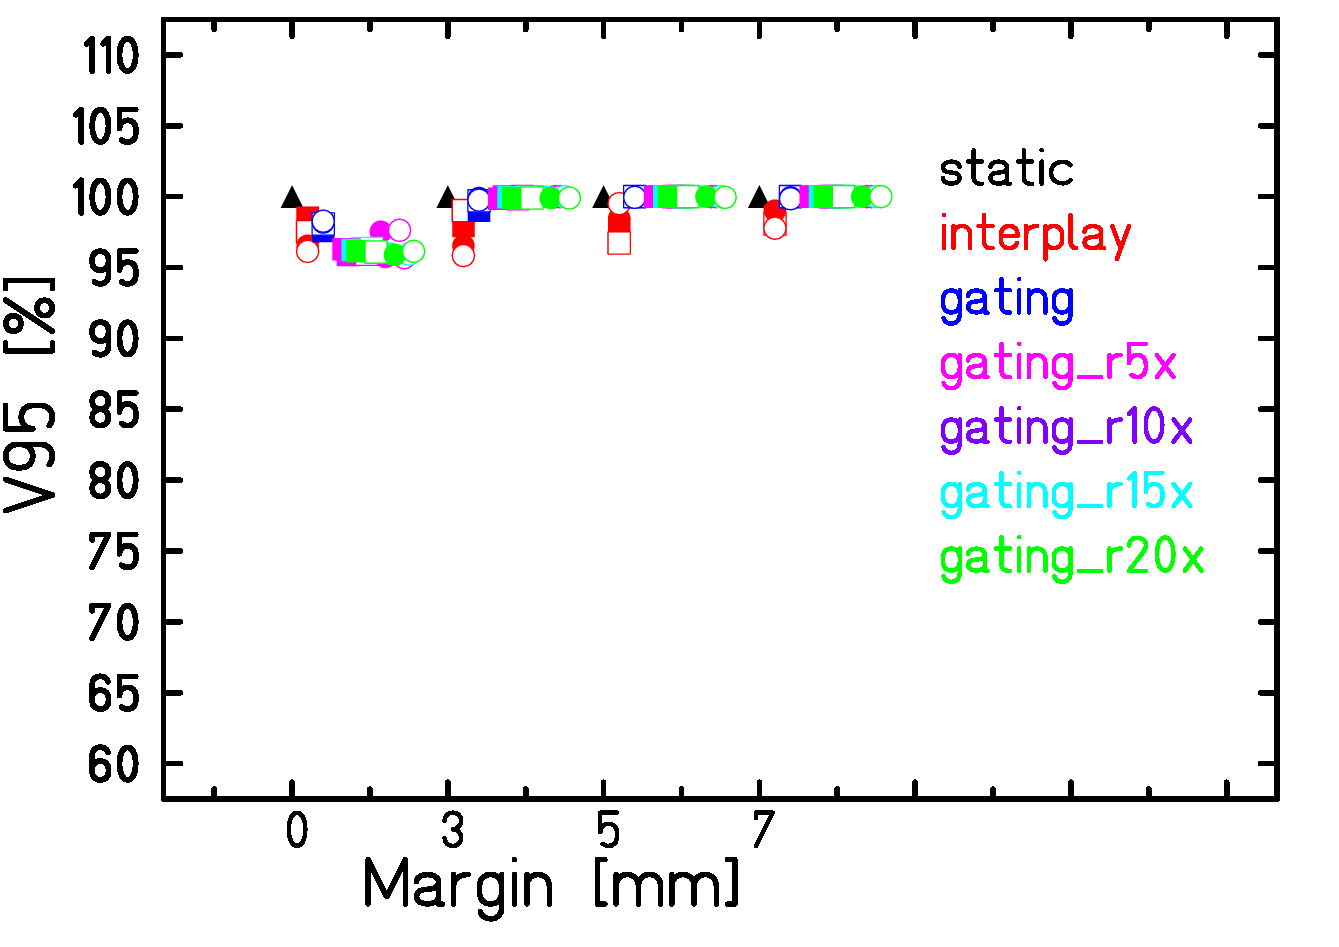
\includegraphics[scale=0.18]{MDACC_Pat024_CTV_RPV_V95_withRescan.png}
 }
  \subfigure[V107: LPV]{
 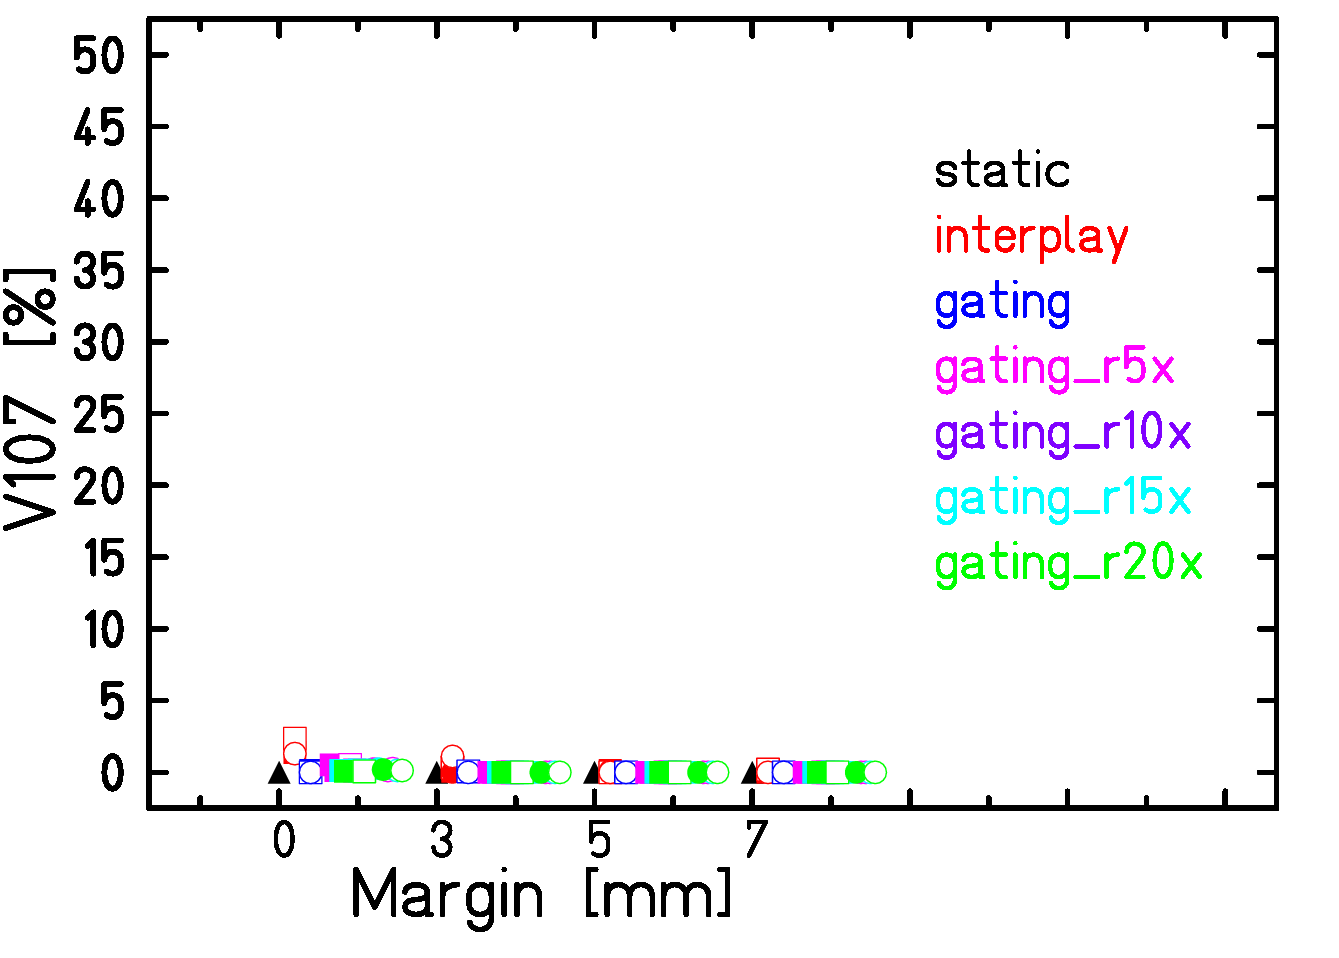
\includegraphics[scale=0.18]{MDACC_Pat024_CTV_LPV_V107_withRescan.png}
 }
\subfigure[V107: RPV]{
 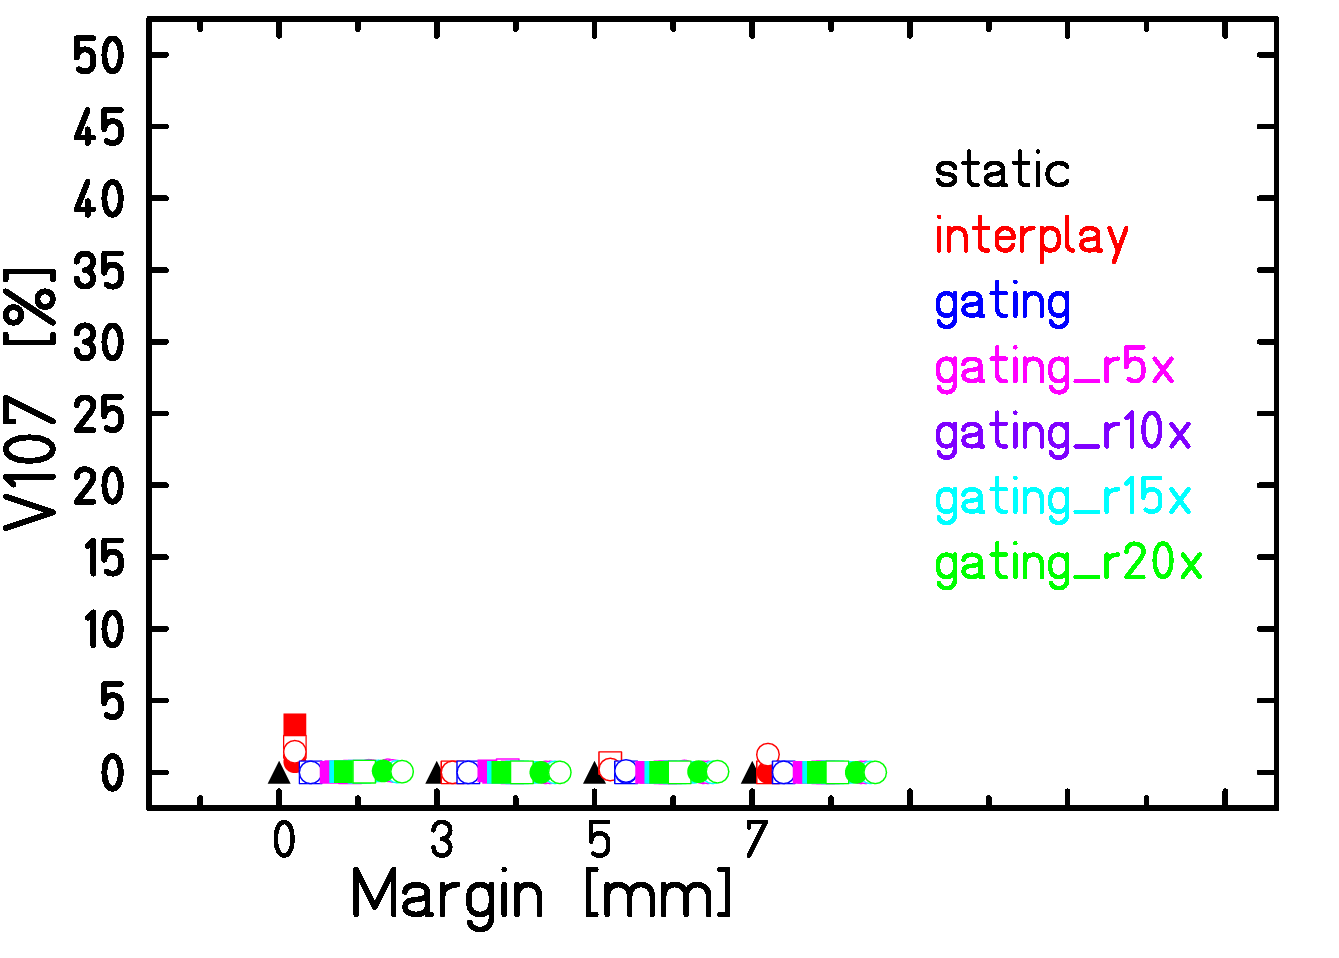
\includegraphics[scale=0.18]{MDACC_Pat024_CTV_RPV_V107_withRescan.png}
 }
\caption{Patient 2: Dose analysis parameters for LPV (left column) and RPV (right column). Besides static (black), interplay (red) and gating 
(blue) also different rescan numbers on the gated irradiation were applied (5 rescans, 10 rescans, 15 rescans and 20 rescans). The results
are compared for four different motions (see figure \ref{static_interplay_gating_Pat01} - \ref{static_interplay_gating_Pat09}) and different 
safety margins.}
\label{static_interplay_gating_rescan_Pat02}
\end{figure}

\begin{figure}[H]
\subfigure[D5-D95: LPV]{
 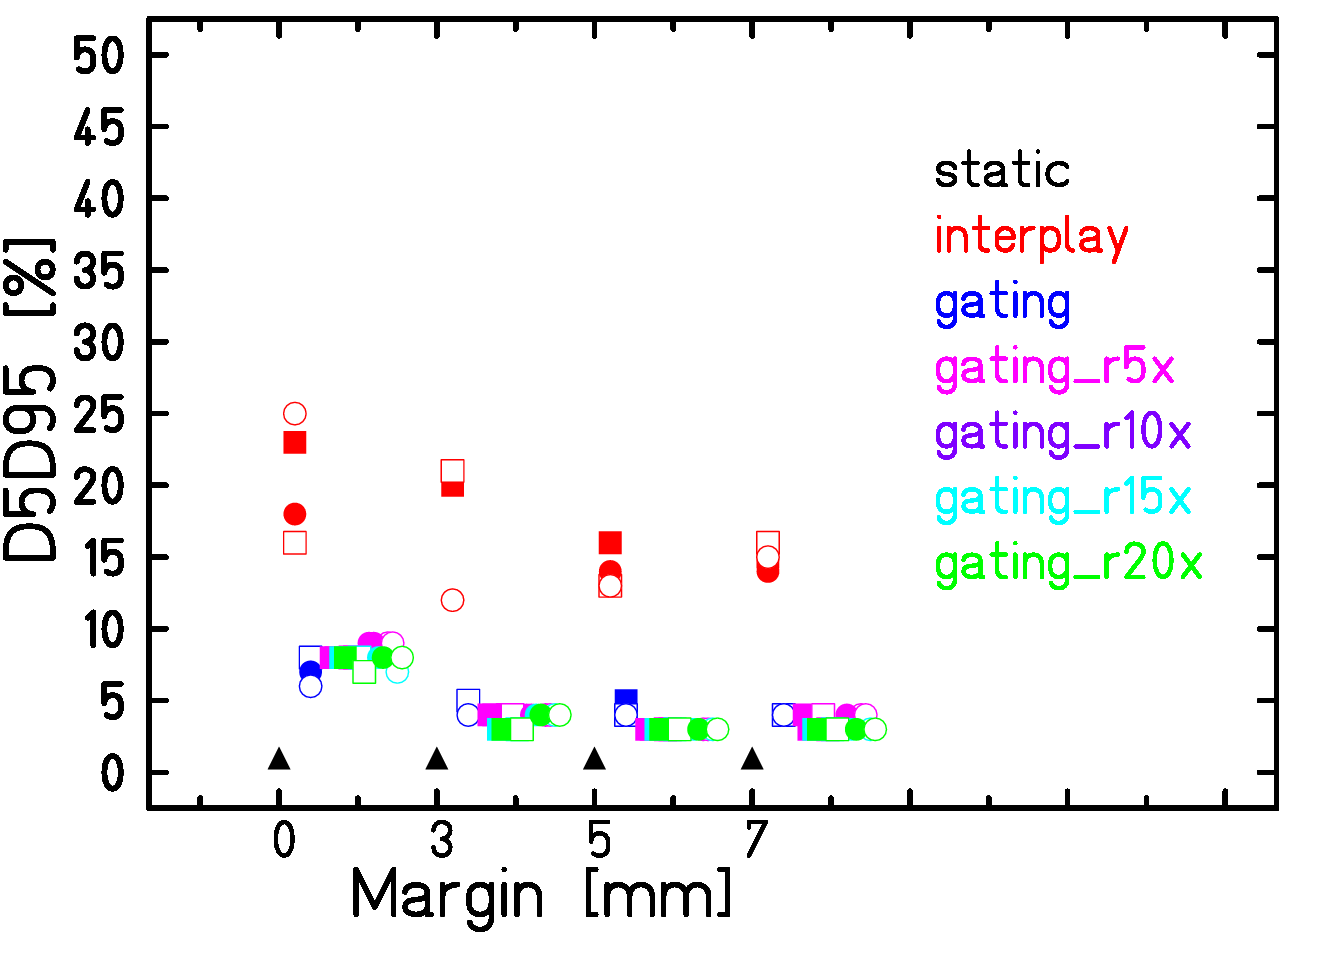
\includegraphics[scale=0.18]{MDACC_Pat122_CTV_LPV_D5D95_withRescan.png}
 }
 \subfigure[D5-D95: RPV]{
 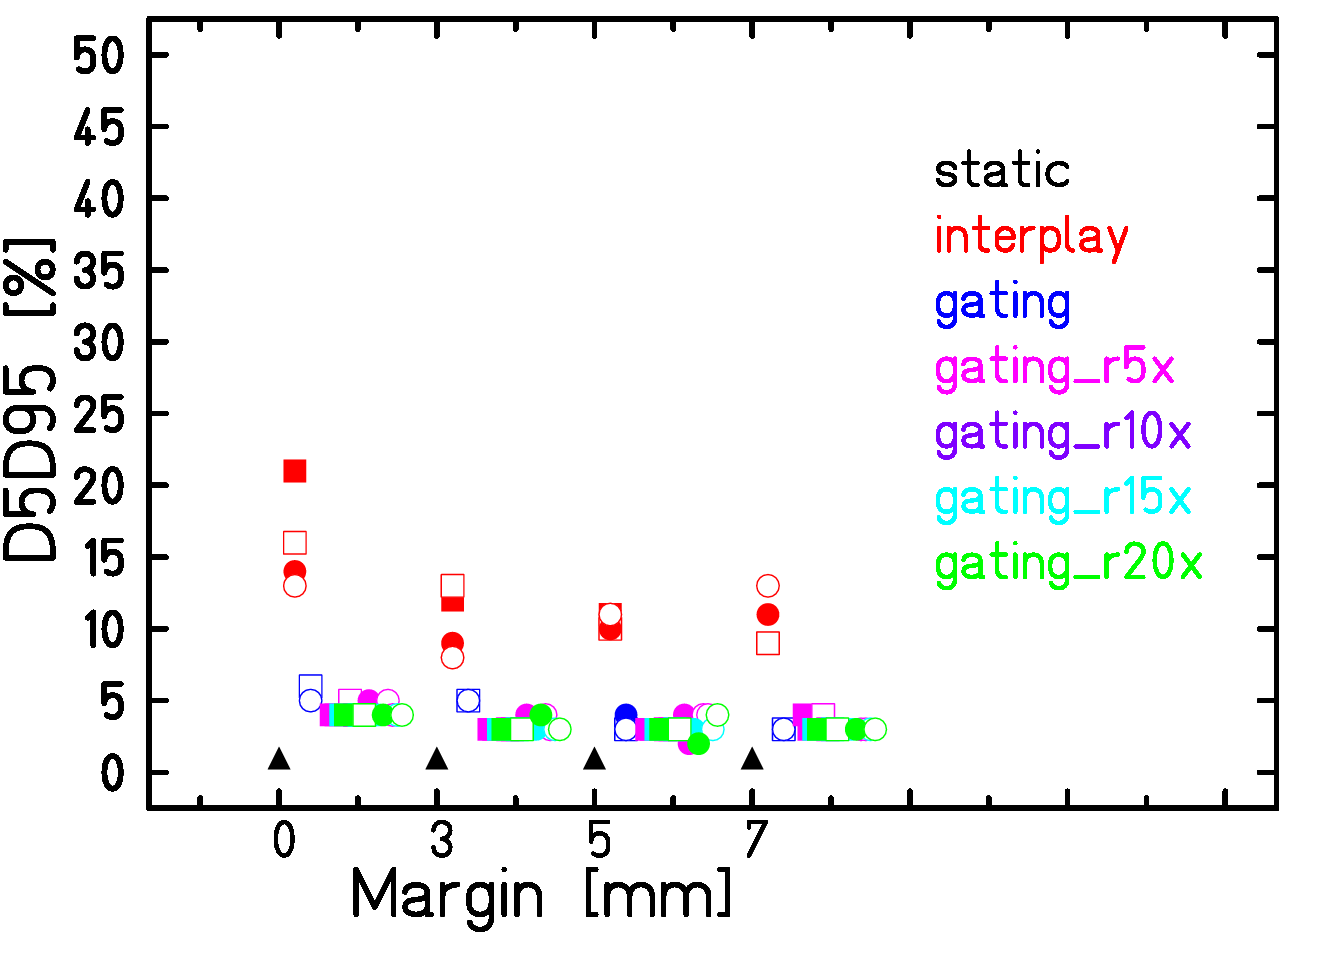
\includegraphics[scale=0.18]{MDACC_Pat122_CTV_RPV_D5D95_withRescan.png}
 }
 \subfigure[V95: LPV]{
 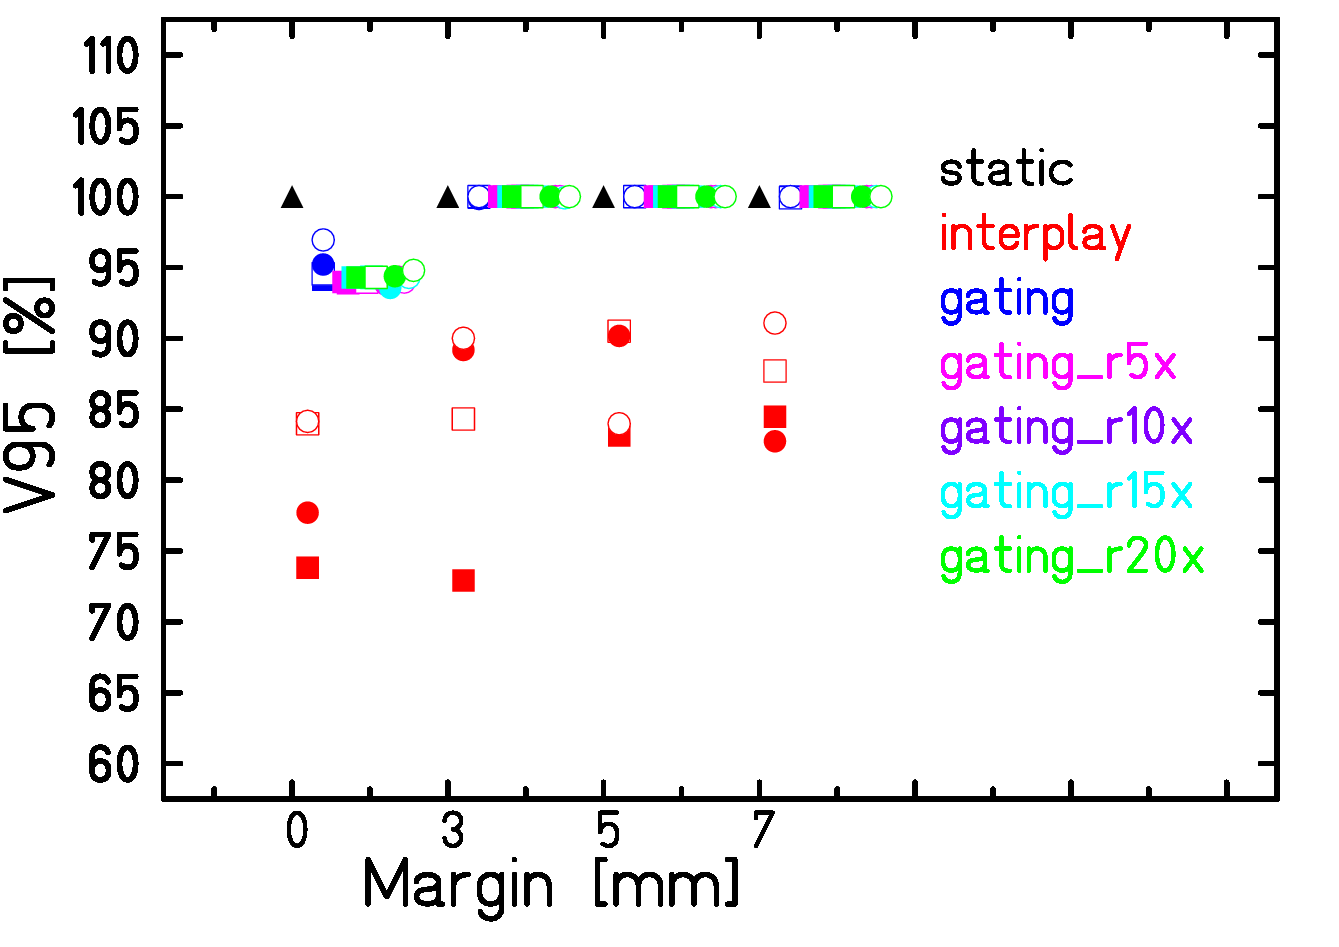
\includegraphics[scale=0.18]{MDACC_Pat122_CTV_LPV_V95_withRescan.png}
 }
\subfigure[V95: RPV]{
 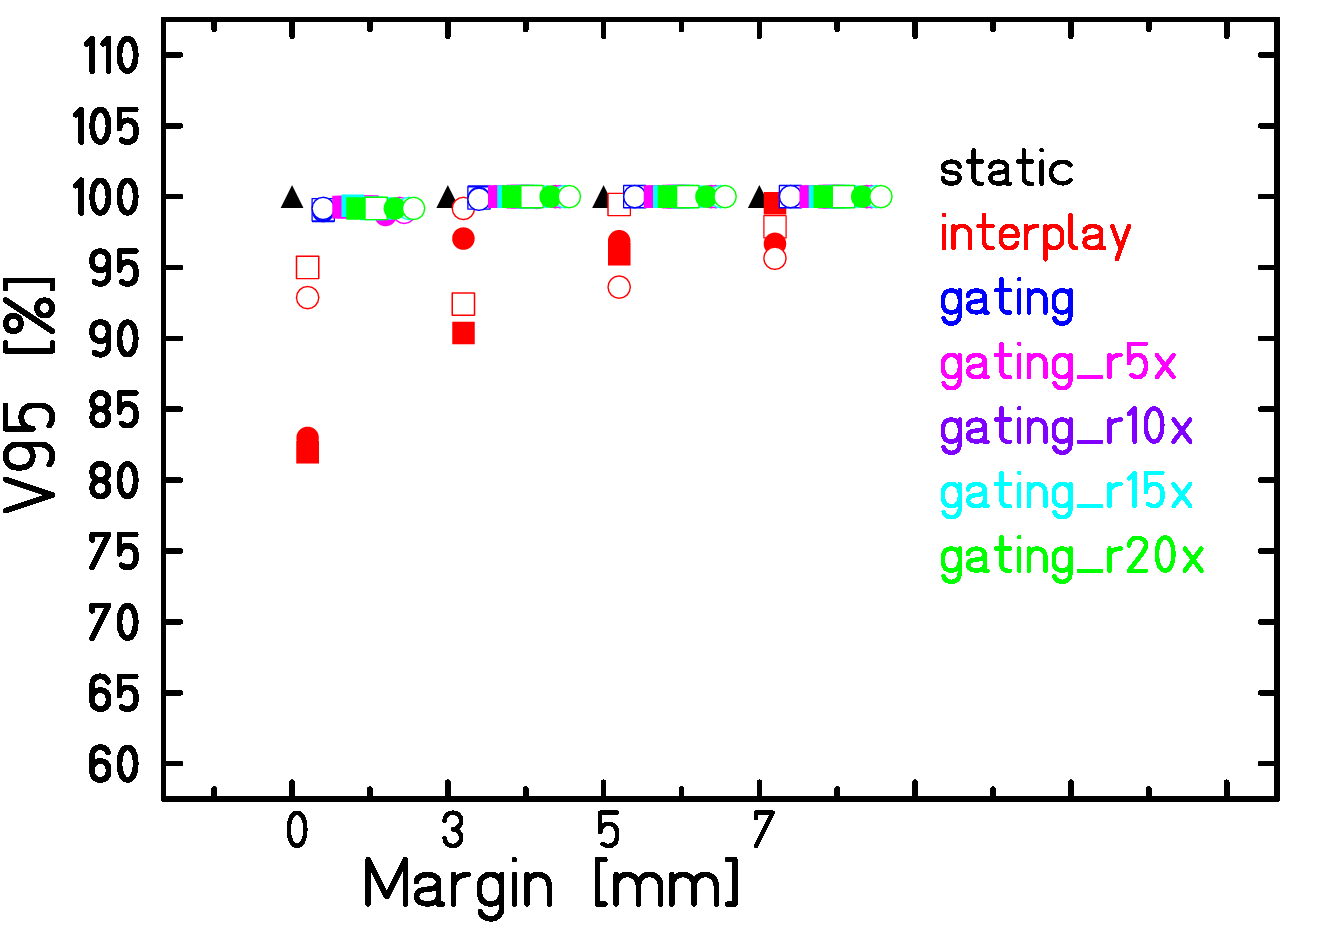
\includegraphics[scale=0.18]{MDACC_Pat122_CTV_RPV_V95_withRescan.png}
 }
  \subfigure[V107: LPV]{
 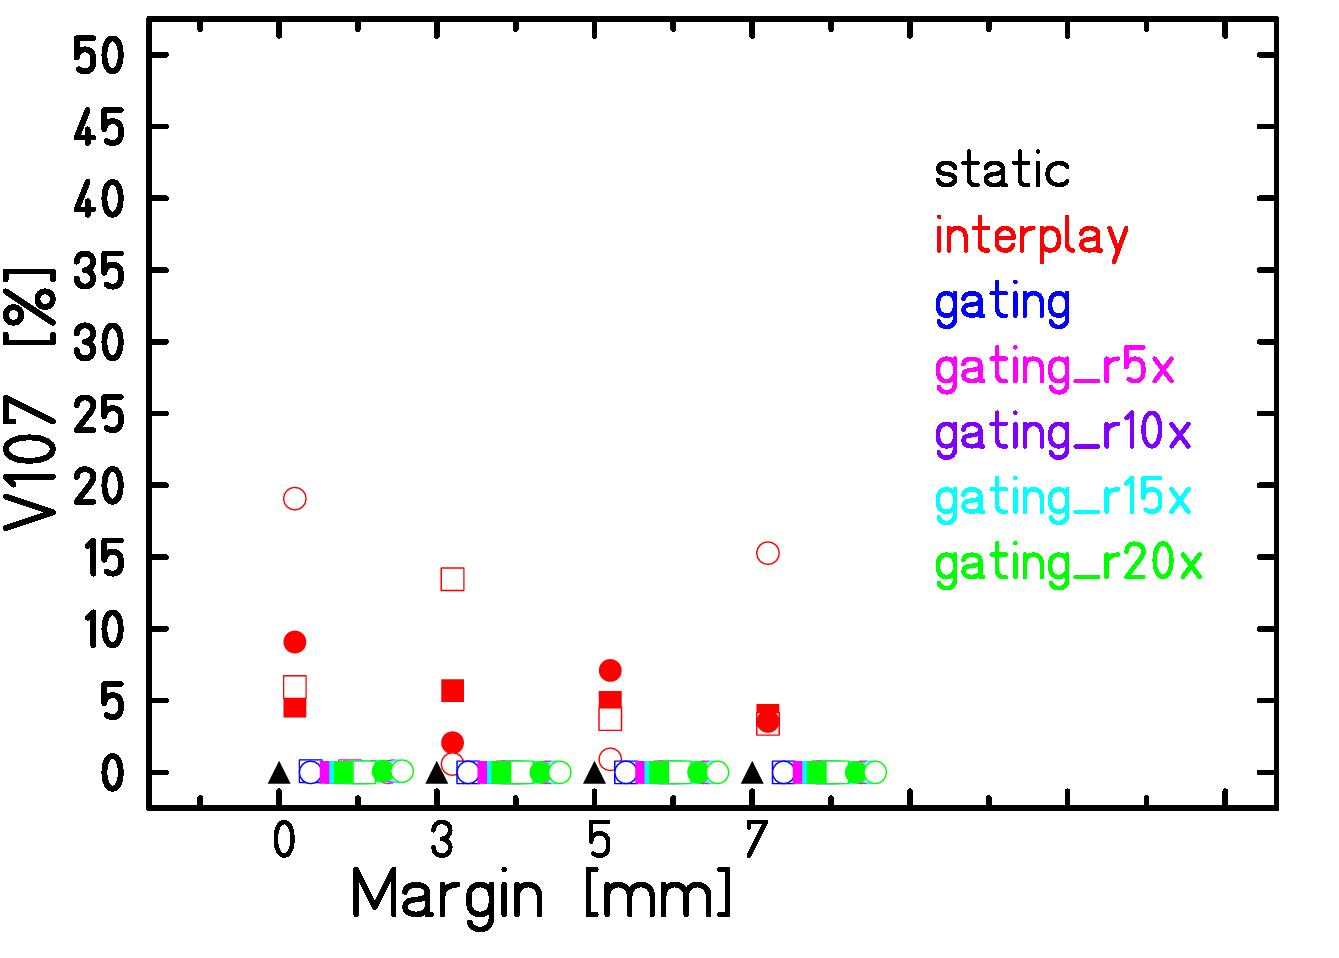
\includegraphics[scale=0.18]{MDACC_Pat122_CTV_LPV_V107_withRescan.png}
 }
\subfigure[V107: RPV]{
 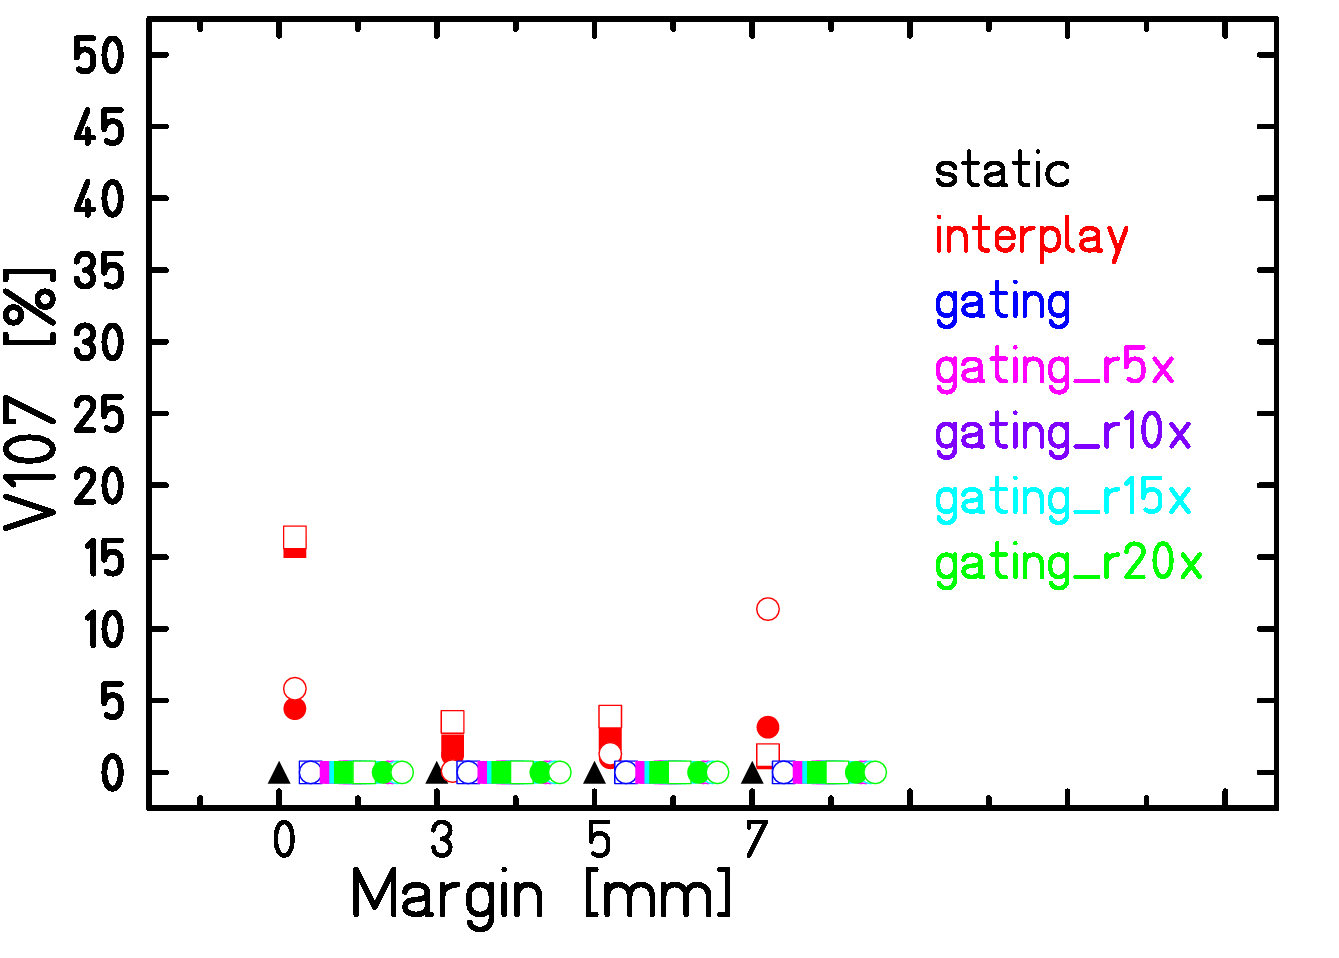
\includegraphics[scale=0.18]{MDACC_Pat122_CTV_RPV_V107_withRescan.png}
 }
\caption{Patient 9: Dose analysis parameters for LPV (left column) and RPV (right column). Besides static (black), interplay (red) and gating 
(blue) also different rescan numbers on the gated irradiation were applied (5 rescans, 10 rescans, 15 rescans and 20 rescans). The results
are compared for four different motions (see figure \ref{static_interplay_gating_Pat01} - \ref{static_interplay_gating_Pat09}) and different 
safety margins.}
\label{static_interplay_gating_rescan_Pat09}
\end{figure}



\newpage

\subsubsection{Irradiation time}

% IRRADIATION TIME
% - plots
% - volume of MDACC contour bigger -> how big ?, influences gating time
% - je groesser margin desto groesser naturlich gating irradiation time
% - motion spielt keinen einfluss
% - nur gating zeit fuer respiration -> zeit um heart beat zu kompensieren in chapter XXX 
% 
% - irradiation time can be increased when increased intensity!!! s. Pat024 -> Plot machen

One of the disadvantages of gating as motion mitigation technique is that the irradiation time is increased depending on the used gating window 
size. When a gating window of roughly 30\% is used, like in this case, the irradiation is prolonged by a factor of three compared to the static 
irradiation. In figure \ref{irrTime_gating_Pat024} the needed irradiation time for the gated irradiation of LPV and RPV in patient 2 is shown for 
different safety margins and motion patterns. The duration for each beam entry channel (gantry angle of -45$^{\circ}$, 135$^{\circ}$ and 0$^{\circ}$) 
is plotted individually. On the left side the duration of an irradiation with a small minimal particle number (11.000 particles) is shown, 
while on the right side an irradiation with a higher minimal particle number (55.000 particles) is displayed. \newline
\newline
It can be seen that the needed irradiation time increases with the used safety margin as the to irradiated volume increases. Furthermore 
the irradiation time is independent of the motion pattern but varies depending on the used beam entry channel. While the low intensity 
irradiation can take up to 120 minutes (for safety margin of 3mm), the overall duration can be reduced to only 30 minutes (for safety margin 
of 3mm) for the irradiation with a higher intensity. It should be noted that this is the gating time for the respiratory motion alone and 
the overall treatment time will thus be prolonged, as cardiac motion is not yet compensated for. 

\vspace*{0.6cm}

% \begin{figure}[H]
% \subfigure[Patient 1]{
%  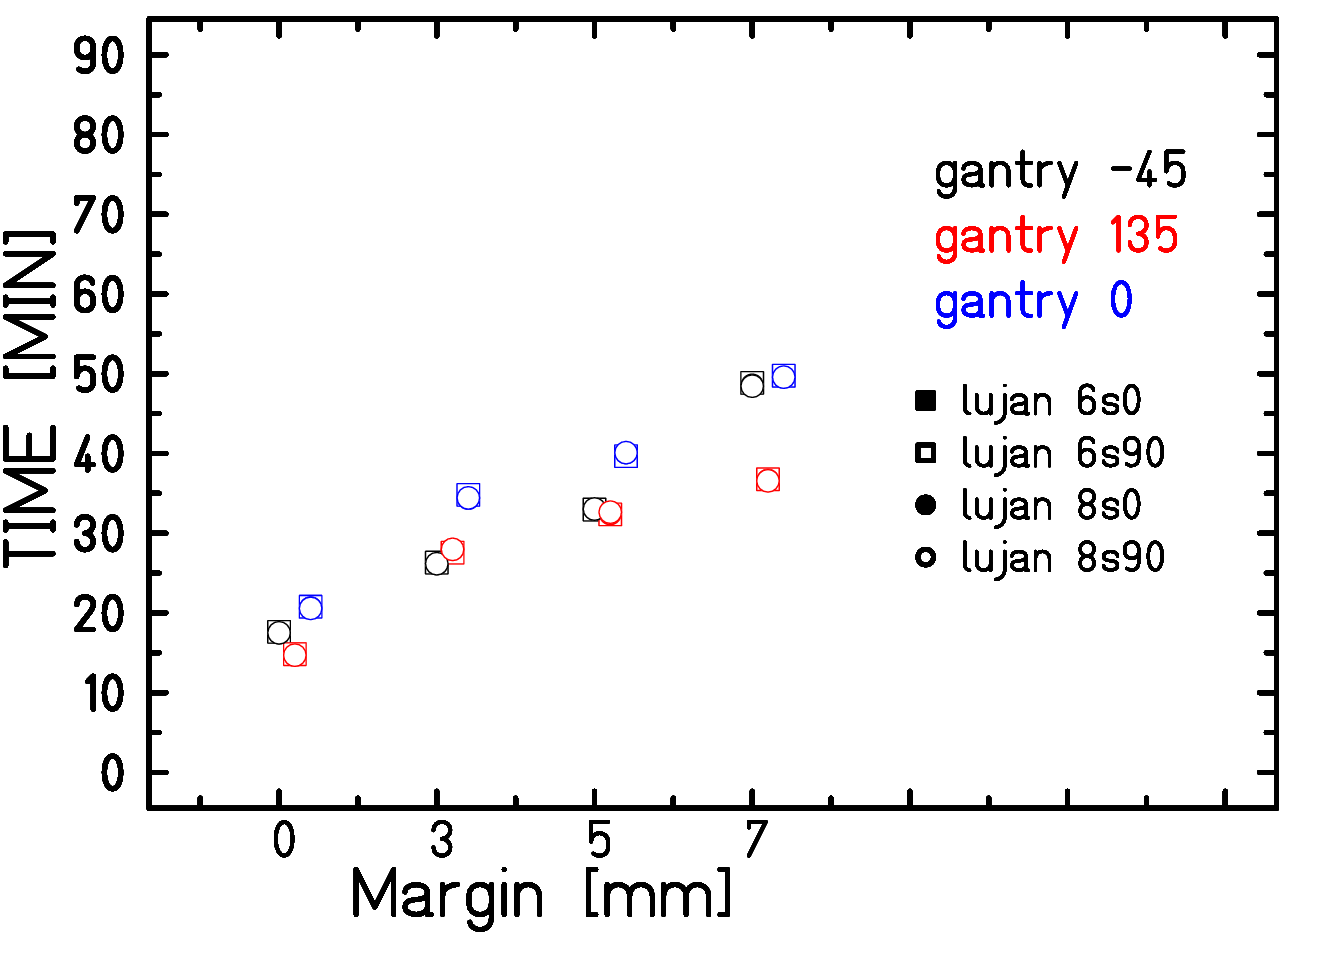
\includegraphics[scale=0.18]{Pat023_all_irrTime.png}
%  }
%  \subfigure[Patient 2]{
%  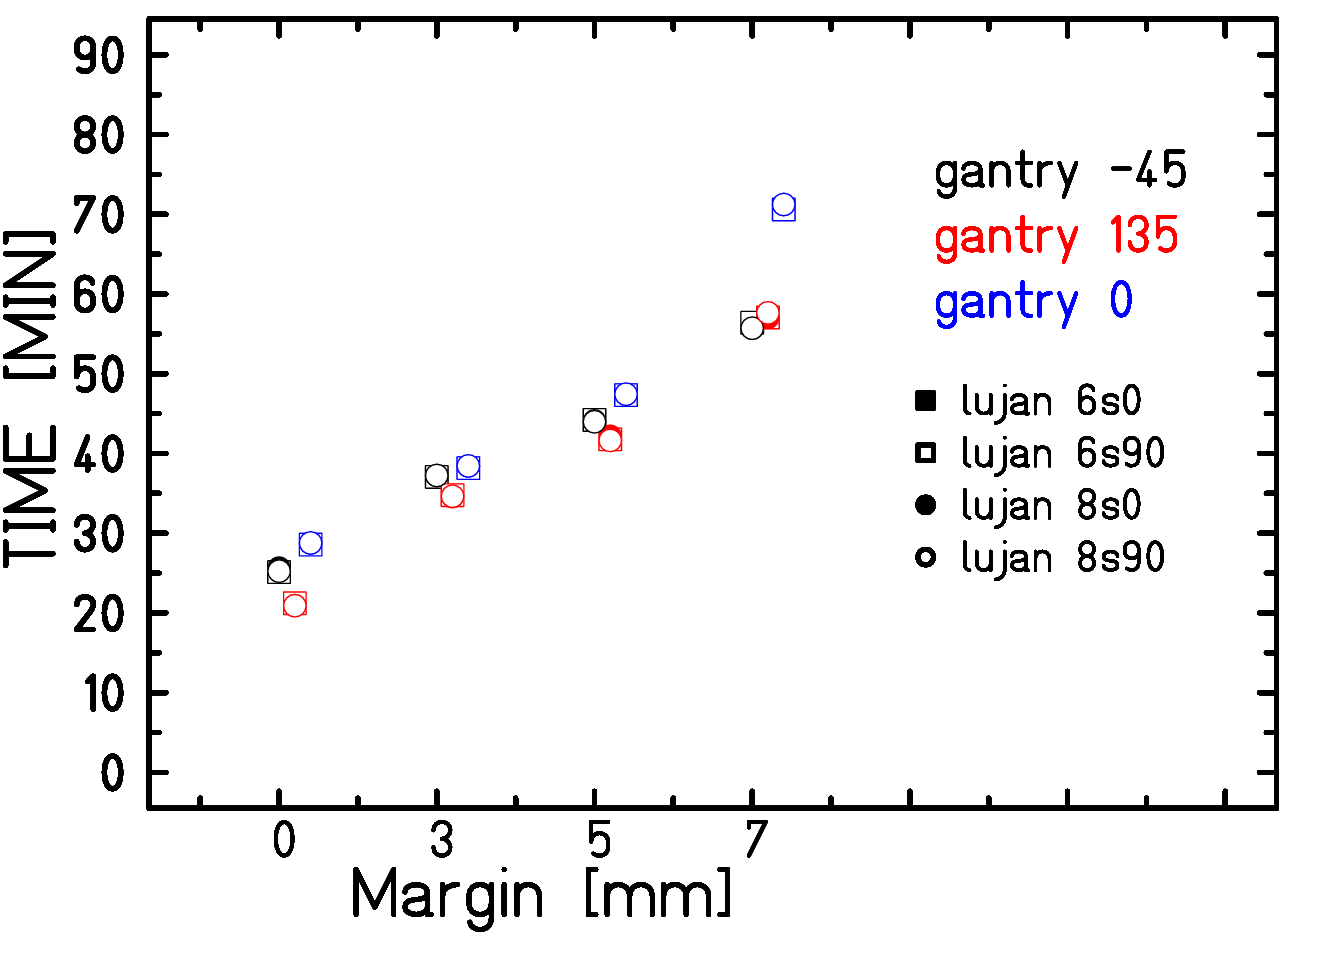
\includegraphics[scale=0.18]{Pat024_all_irrTime.png}
%  }
% \subfigure[Patient 3]{
%  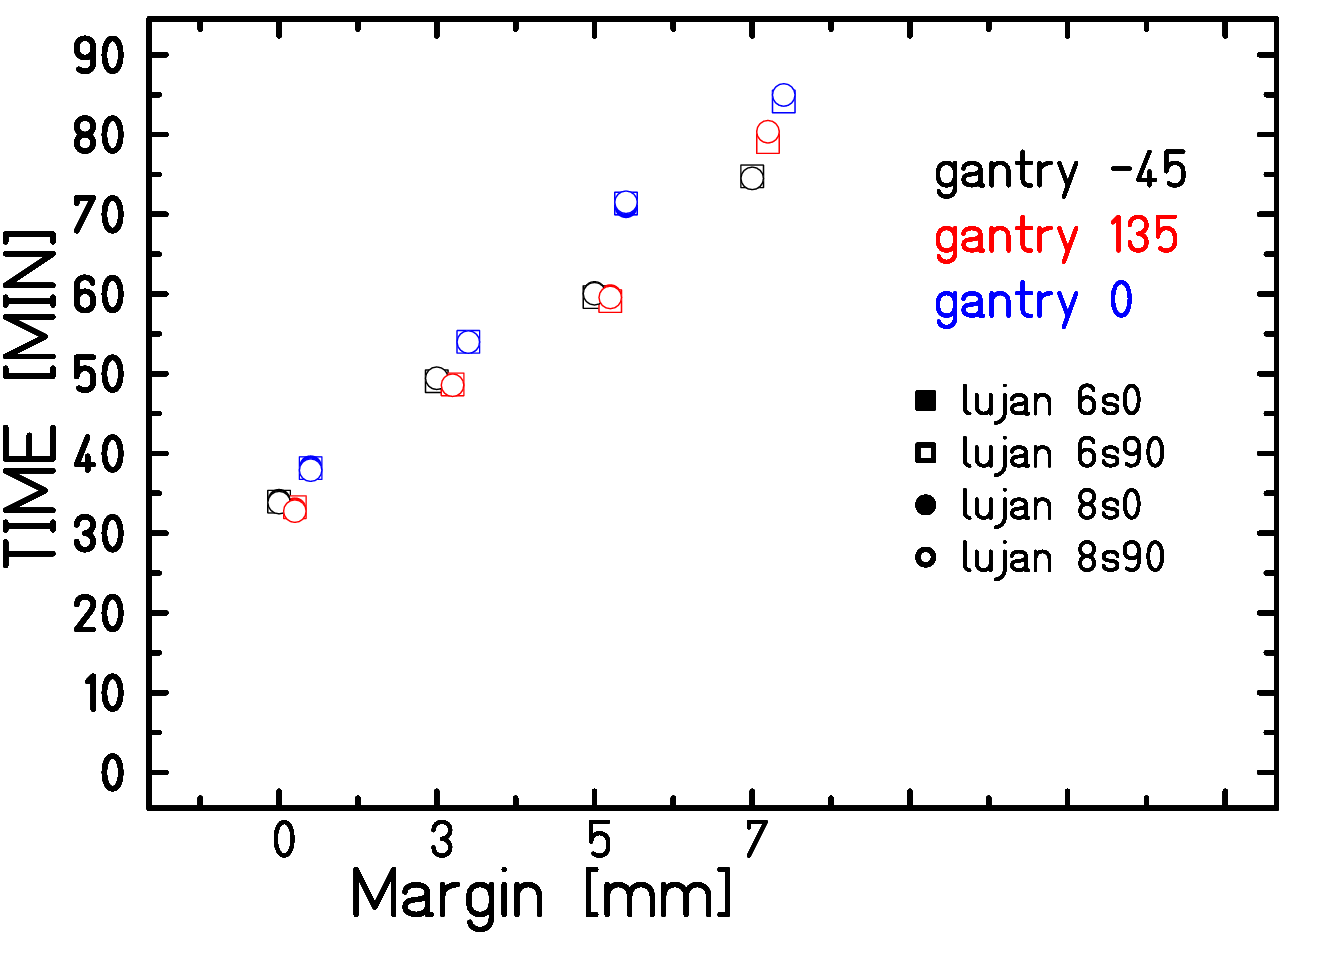
\includegraphics[scale=0.18]{Pat026_all_irrTime.png}
%  }
% \subfigure[Patient 4]{
%  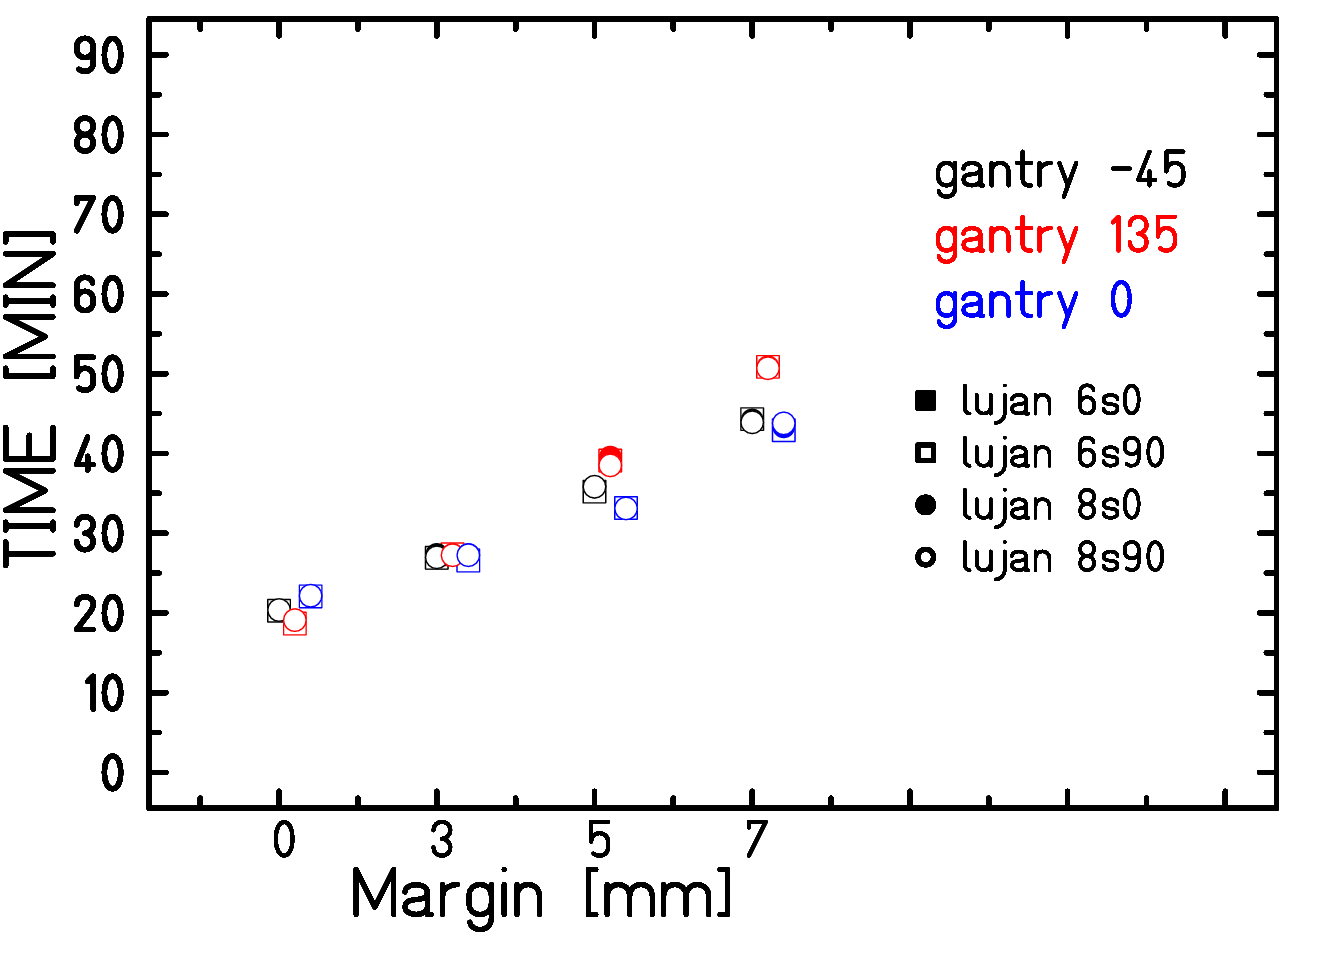
\includegraphics[scale=0.18]{Pat031_all_irrTime.png}
%  }
%  \subfigure[Patient 5]{
%  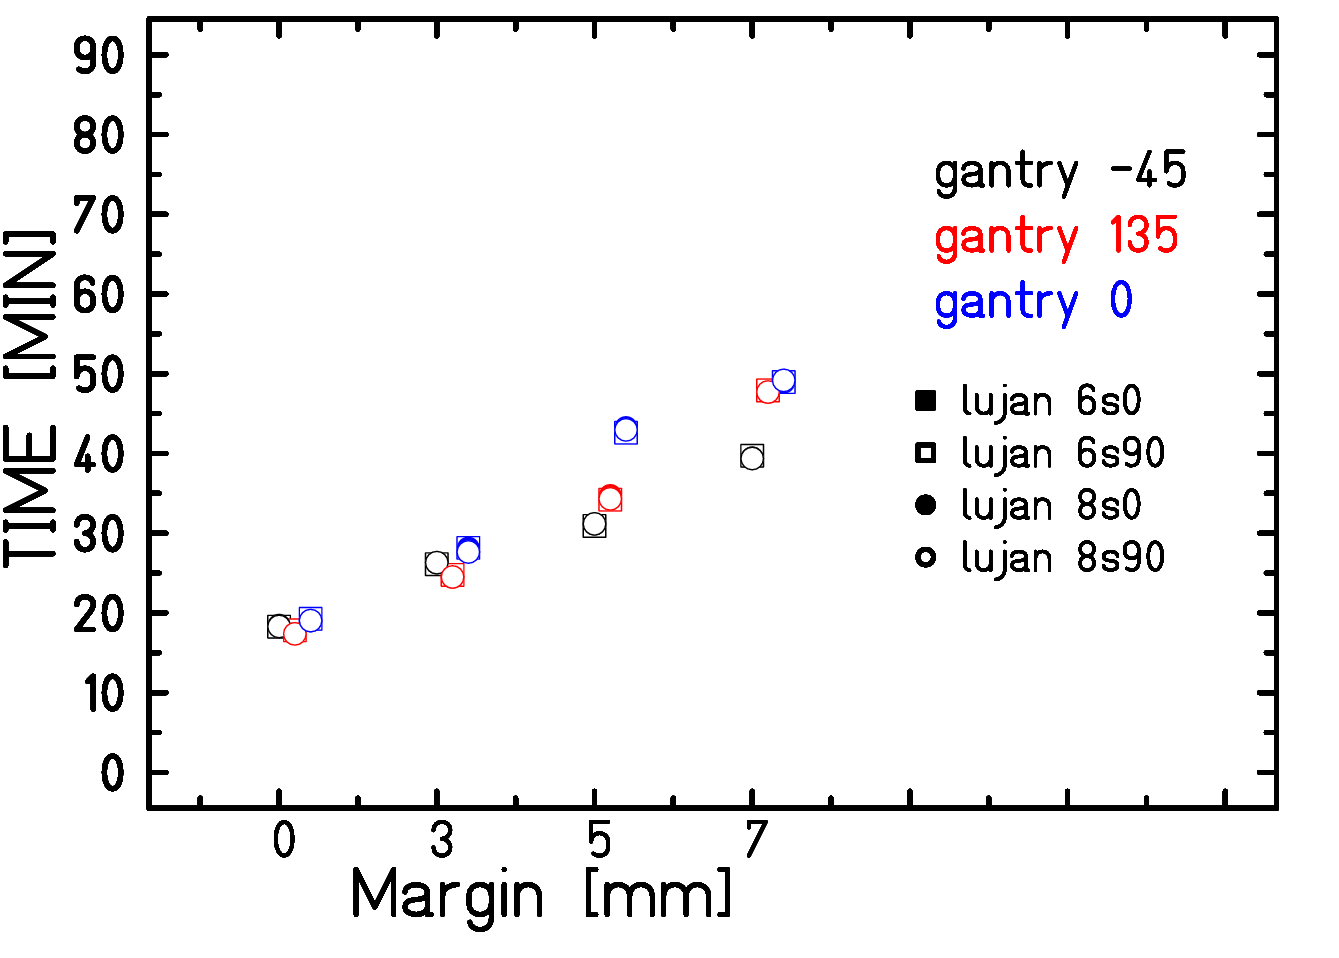
\includegraphics[scale=0.18]{Pat035_all_irrTime.png}
%  }
%  \subfigure[Patient 6]{
%  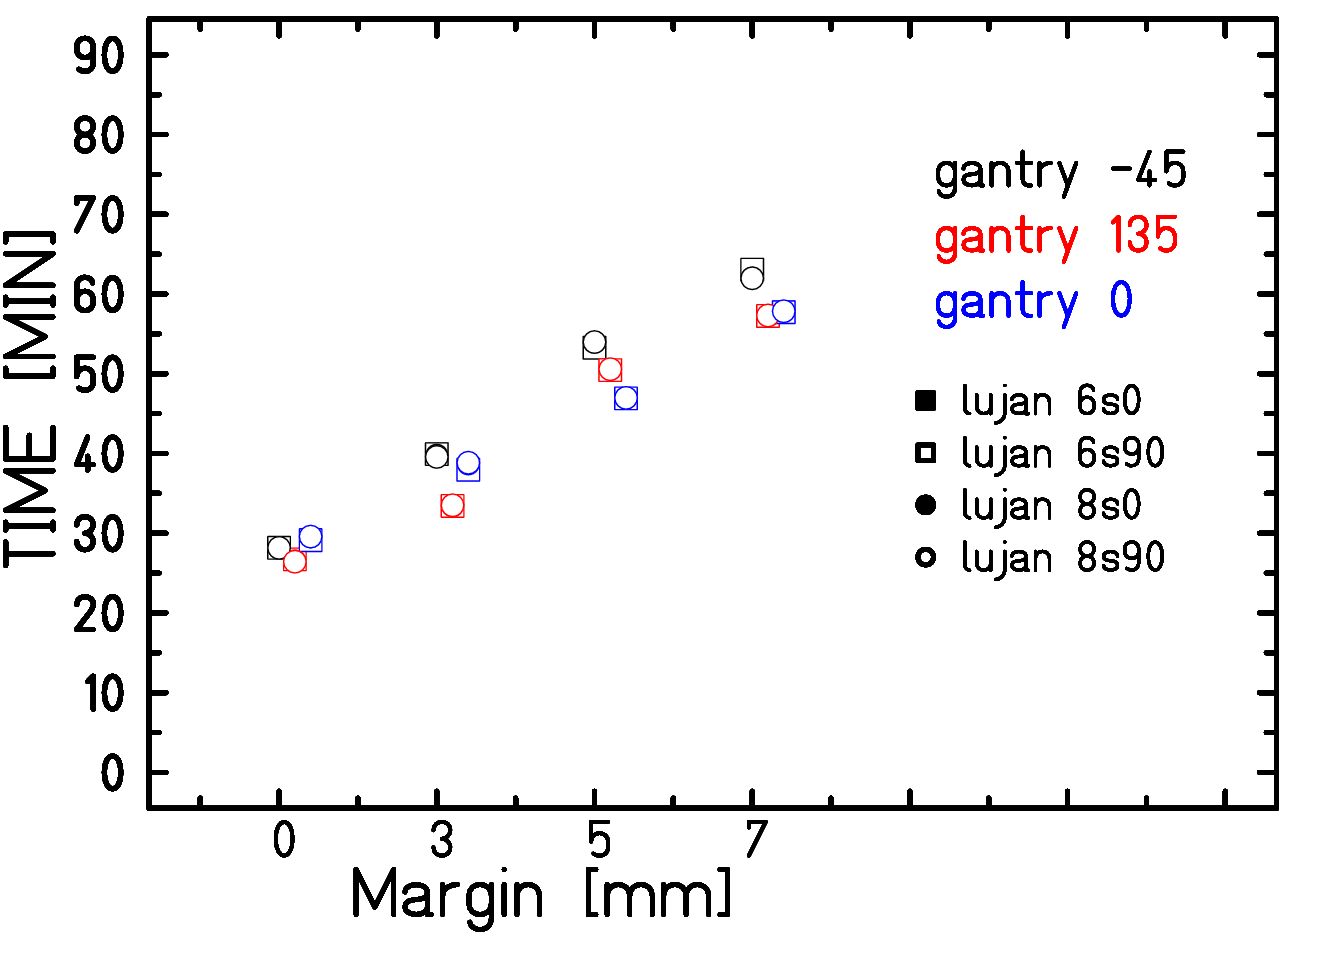
\includegraphics[scale=0.18]{Pat036_all_irrTime.png}
%  }
%  \caption{Irradiation time for gating for patients 1 - 6. The irradiation time is displayed for each beam direction seperately (gantry angle -45: 
% black, gantry angle 135: red, gantry angle 0: blue) as well as for four different motion types. The irradiation time is meant as time 
% needed for the irradiation of LPV and RPV together for every respective case.}
% \label{irrTime_gating}
% \end{figure}
 
%  \begin{figure}[H]
% \subfigure[Patient 7]{
%  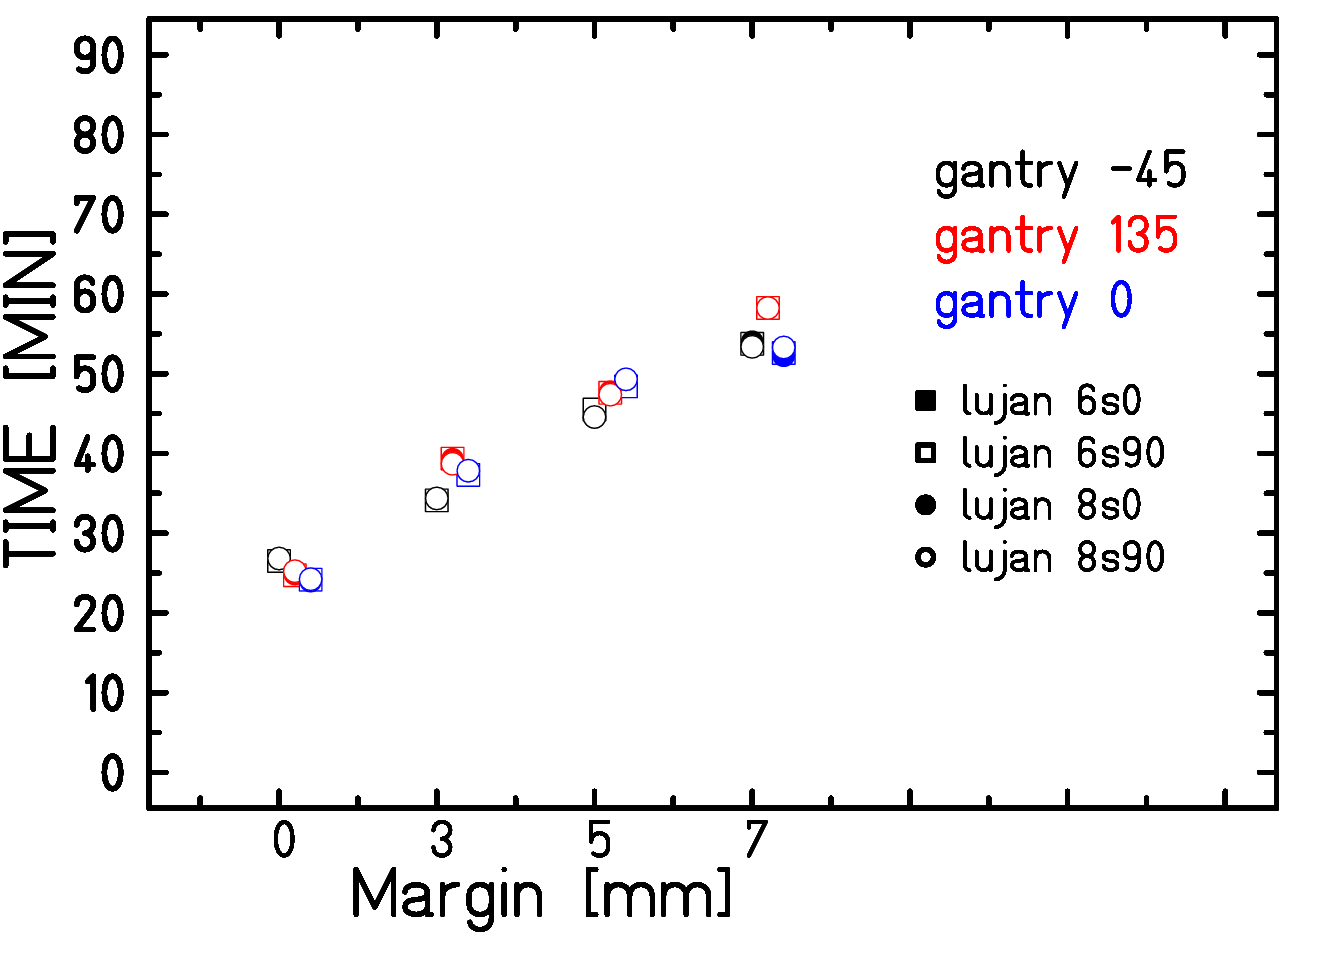
\includegraphics[scale=0.18]{Pat037_all_irrTime.png}
%  }
% \subfigure[Patient 8]{
%  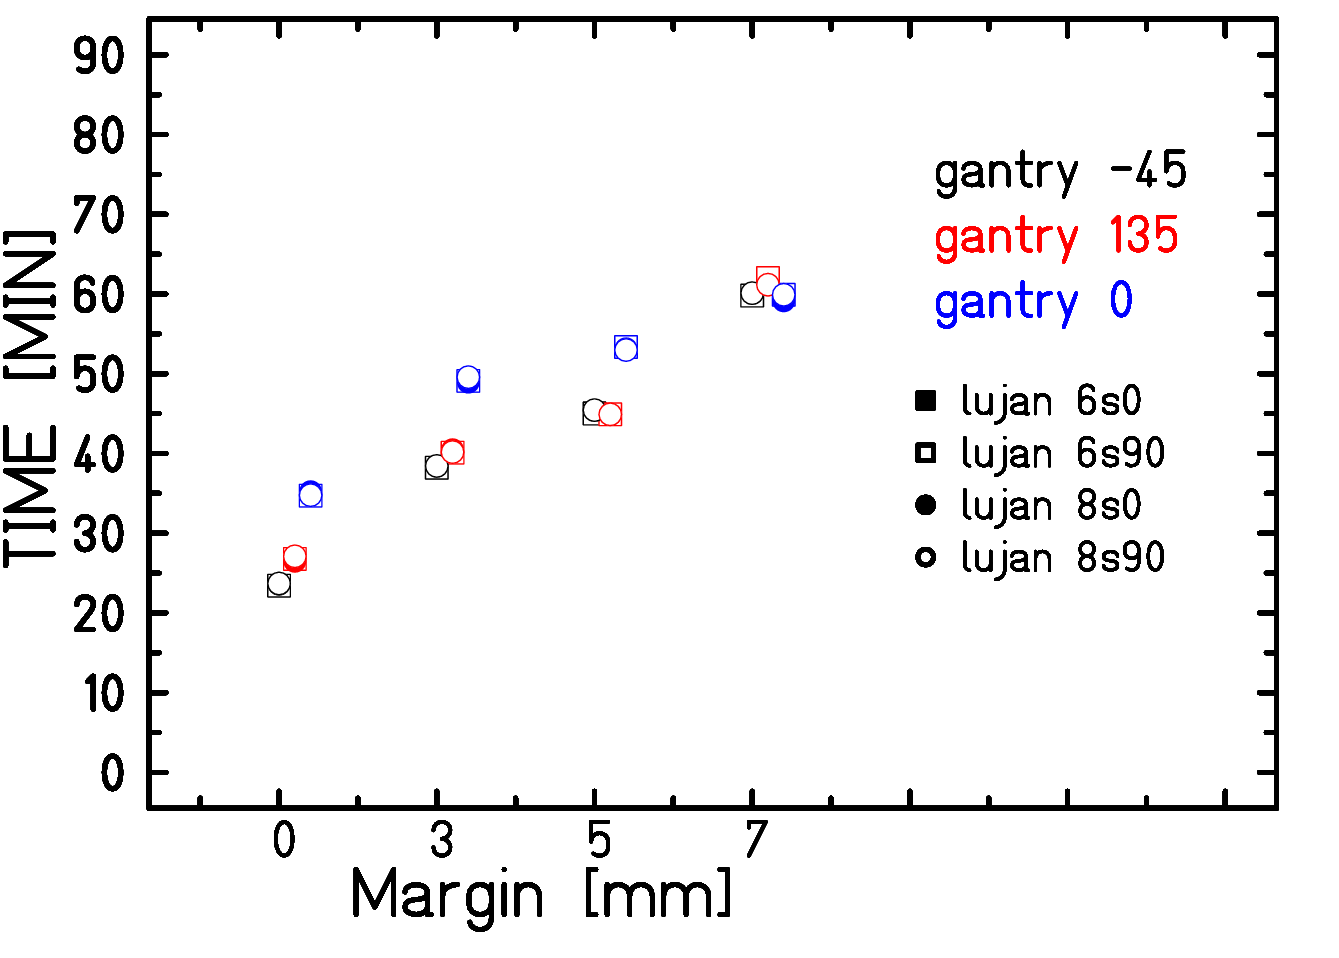
\includegraphics[scale=0.18]{Pat039_all_irrTime.png}
%  }
%  \subfigure[Patient 9]{
%  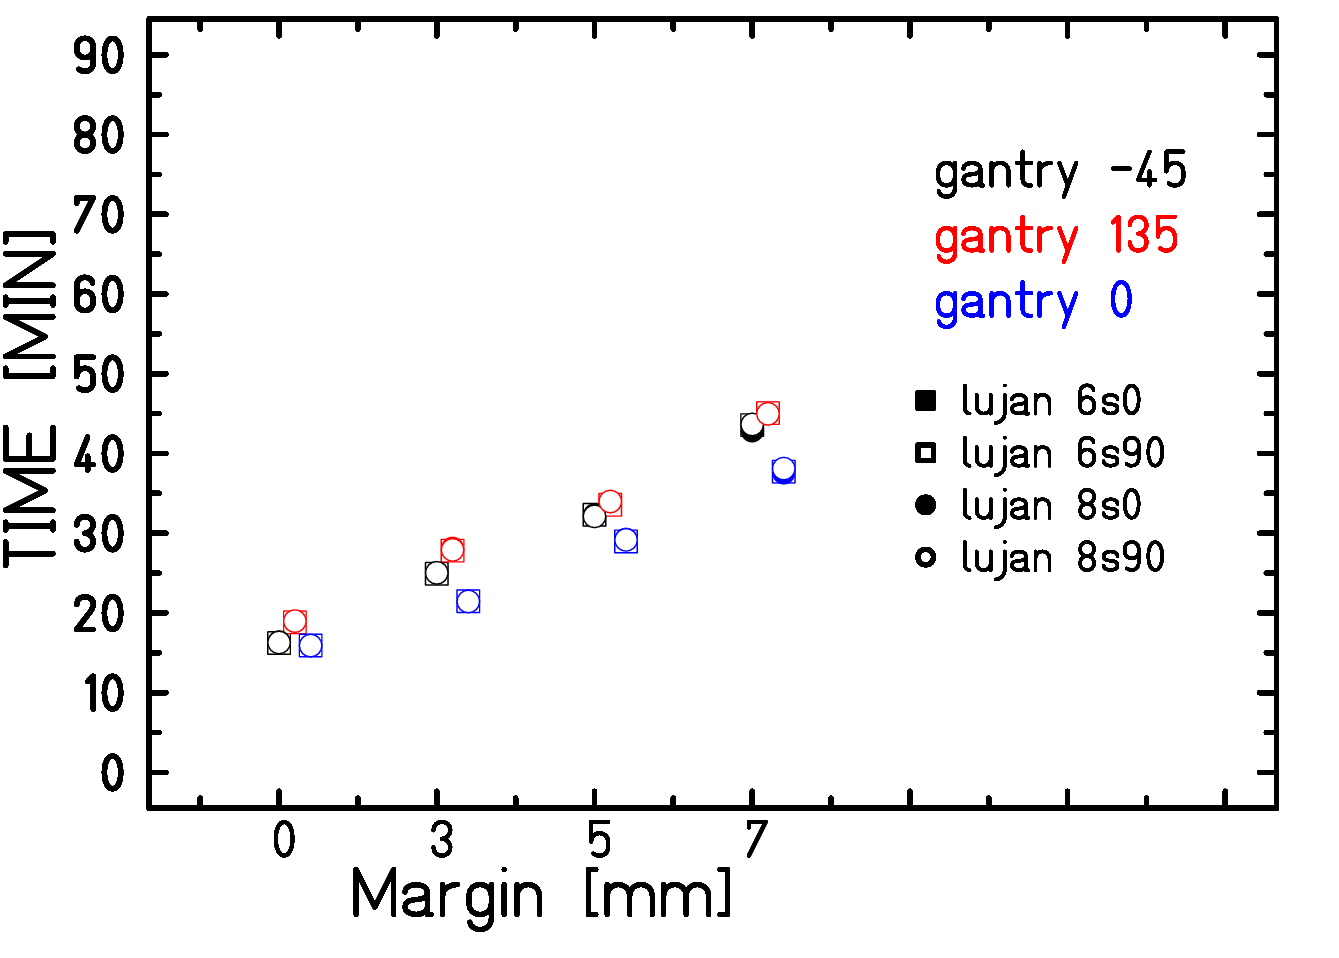
\includegraphics[scale=0.18]{Pat122_all_irrTime.png}
%  }
% \caption{Irradiation time for gating for patients 7 - 9. The irradiation time is displayed for each beam direction seperately (gantry angle -45: 
% black, gantry angle 135: red, gantry angle 0: blue) as well as for four different motion types. The irradiation time is meant as time 
% needed for the irradiation of LPV and RPV together for every respective case.}
% \label{irrTime_gating_2}
% \end{figure}

 \begin{figure}[H]
\subfigure[Patient 2: smaller intensity]{
 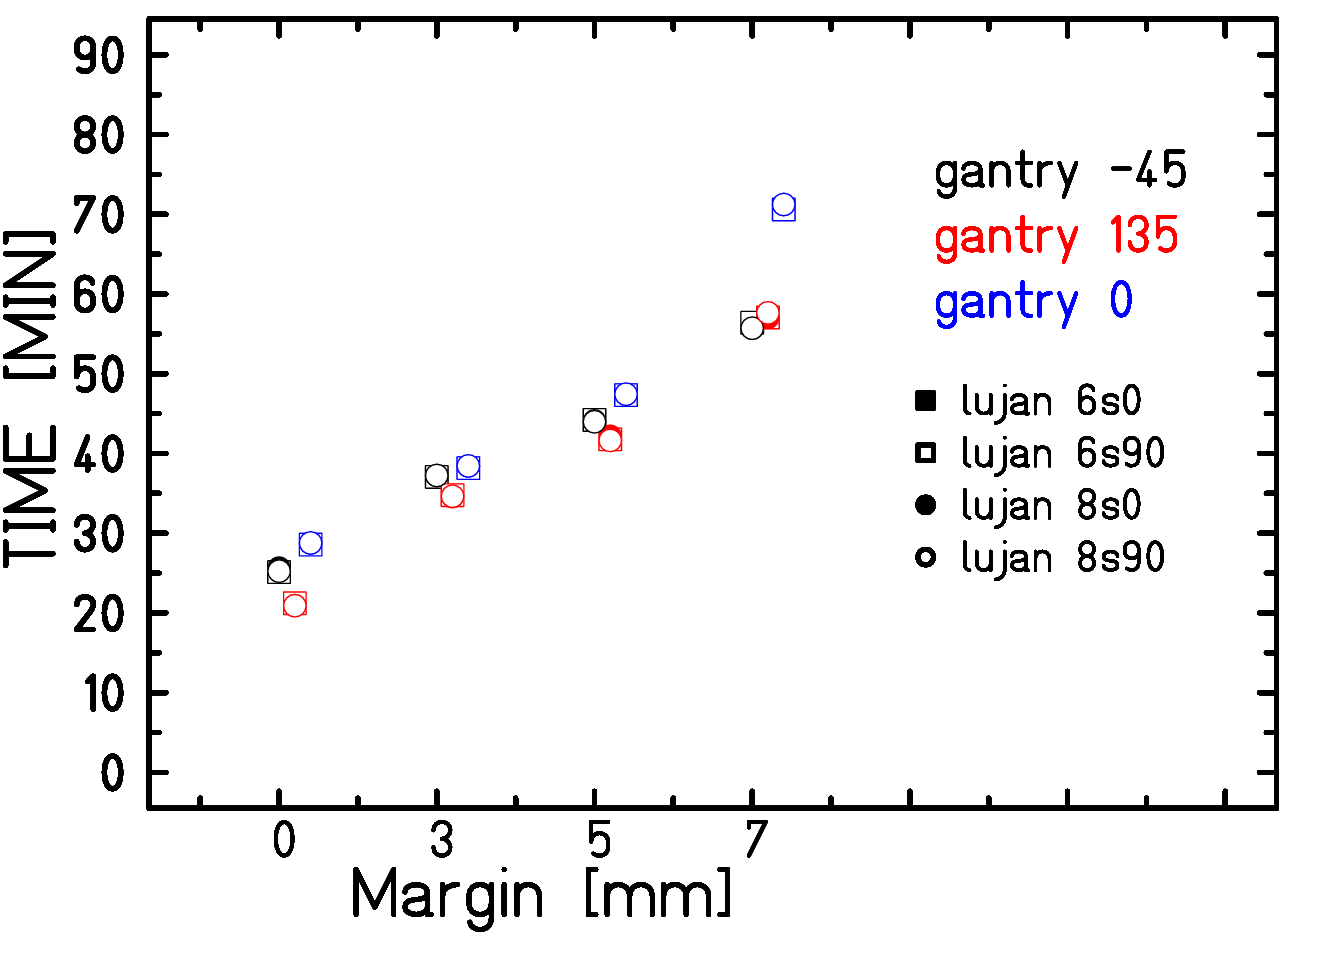
\includegraphics[scale=0.18]{Pat024_all_irrTime.png}
 }
\subfigure[Patient 2: higher intensity]{
 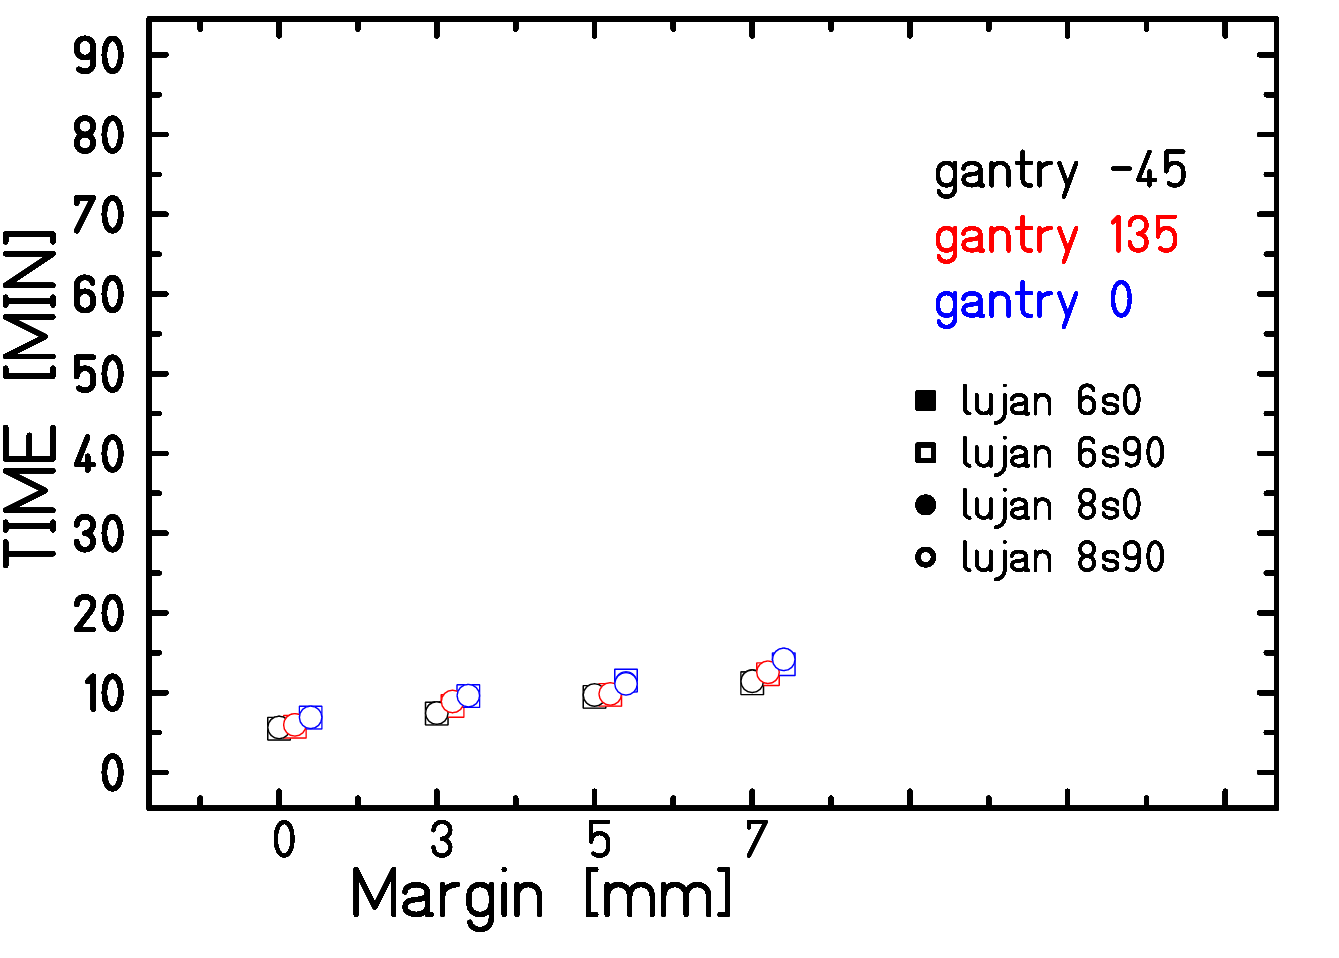
\includegraphics[scale=0.18]{Pat024_all_irrTime_hoheNmin.png}
 }
\caption{Irradiation time for gating for patient 2 for different intensities (Nmin = 11.000 (left) and Nmin = 55.000 (right)), different 
safety margins, underlying motion patterns and beam entry channels.}
\label{irrTime_gating_Pat024}
\end{figure}



\newpage

\section{Discussion}
In this chapter the influence of respiratory motion on the PVs was studied and treatment planning studies with gating as motion 
mitigation technique were carried out. Respiration was found to be an important motion component for the treatment of cardiac volumes. 
Recent studies in the cardiology community also indicate that real time compensation of breathing displacement 
would even be beneficial for catheter ablation \cite{Kum12} \cite{Frie12}.\newline
\newline
Different studies on the influence of respiration on the PV motion exist as they are of interest for image guided ablation procedures. 
Thereby relative displacements (like deformation or splaying of the PVs) and absolute motion (translational and rotation) are distinguished. 
Noseworthy et al. \cite{Nos05} studied the relative changes in the PV anatomy during the breathing cycle. They thereby investigated the changing 
branching angle between the inferior and superior LPV (LIPV, LSPV) and RPV (RIPV, RSPV), respectively. They stated that the PV splay during 
inspiration (branching angle of RPVs increased from (40 $\pm$ 10)$^\circ$ to (60 $\pm$ 15)$^\circ$ in inspiration and for LPVs 
from (50 $\pm$ 11)$^\circ$ to (62 $\pm$ 13)$^\circ$ in inspiration). Furthermore they found a significant reduction in 
the diameter of the RIPV and RSPV during inspiration. Ector et al. \cite{Ect08} on the other hand stated that they only found a slight, 
but significant diameter reduction in the RIPV. In their paper they furthermore studied the absolute translational motion. 
Their patient cohort had a mean diaphragmatic movement of (35 $\pm$ 16)mm for the right diaphragm, resulting in an absolute mean displacement 
for both LPV and RPV of (19.1 $\pm$ 8.6)mm. The mean inferior motion was stated 
to (14.6 $\pm$ 7.7)mm, in anterior direction to (9.7 $\pm$ 7.6)mm and the smallest motion direction was the leftward direction with 
(0.4 $\pm$ 3.8)mm. Comparing motion patterns between veins the LPVs were found to move less in anterior direction then the RPVs, but did 
not differ significantly in other directions. They found a strong association between diaphragmatic motion and inferior PV motion.\newline
\newline
% Noseworthy et al. and Ector et al. both stated that respiration causes important movements of the PVs. They concluded that errors in image-guided 
% therapy can only be avoided when the respiratory motion phase is carefully considered. Real-time correction of respiratory motion components 
% in fluoroscopic images is however not available at present \cite{Ect08}. \newline
% \newline
% A recent study by Kumar et al. \cite{Kum12} investigated the effect caused by respiration on catheter tip contact force during ablation and 
% hence on the treatment outcome. Patients for CTI ablation for atrial flutter as well as PV ablation for atrial fibrillation were 
% treated during artifical breathing (ventilation or apnea). The patients were under general anesthesia and intubated, spontaneous respiration 
% did not occur. It was stated that the average force as well as the force-time integral were significantly higher with apnea compared to 
% ventilation. This was attributed to a drop in catheter tip contact force due to respiratory motion in ventilation. Catheter contact 
% force has a significant impacts on the energy transfer and hence lesion creation \cite{Frie12} \cite{Shah10} \cite{Yok08}. Low contact force 
% as well as low force-time interval are connected to conduction recovery \cite{Vij10} \cite{Red11} \cite{Shah11}. It could thus be concluded 
% that respiration plays an important role in lesion creation and that complications may be minimized by considering the respiratory motion. 
% Besides ventilation and apnea, Friedmann \cite{Frie12} also states that jet ventilation or breath-hold might be adequate strategies for 
% catheter ablation. 
% \newpage
In the here studied patient cohort of lung cancer patients a much smaller mean absolute displacement of the pulmonary veins was found over all patients with 
(6.76 $\pm$ 3.57)mm for LPV and (6.76 $\pm$ 2.51) for RPV. The SI motion was found to (-6.41 $\pm$ 3.80)mm and (-6.57 $\pm$ 2.42)mm for RPV, 
respectively. In AP direction the mean amplitude for all patients was found to (-0.81 $\pm$ 0.54)mm for LPV and (-0.94 $\pm$ 0.84) for RPV, 
which corresponds to the finding by Ector et al. that the LPV move less in anterior direction than the RPV. For LR direction 
a mean displacement of (-0.93 $\pm$ 0.89) of LPV and (0.48 $\pm$ 1.02)mm of RPV was found over all patients. 
Contrary to Ector et al. a significant difference in the motion of the LPV compared to RPV was hence found in LR. 
A strong correlation between diaphragm motion and PV displacement was only found in the RPV (r=0.79, p<0.05). Even though a similar result 
was expected for the LPV, no correlation was observed here. It is unclear if this is due to location of the ablation site or the 
underlying lung cancer patient data in comparison to AF patient data sets.\newline
\newline
Recent studies in the cardiology community \cite{Kum12} concluded that also for catheter ablation respiration plays an important role as it may 
reduce the catheter tip contact force. Consideration of respiratory motion is thus recommended. Besides ventilation and apnea, Friedmann 
\cite{Frie12} also states that jet ventilation or breath-hold might be adequate strategies for catheter ablation. While the latter may also 
be options for a non-invasive treatment of atrial fibrillation with a scanned carbon ion beam, gating was 
studied as a motion mitigation technique in the here presented work. In irradiation of cardiac volumes in the animal studies carried out 
at CyberHeart and at the Universit\"atsklinikum Schleswig-Holstein in L\"ubeck different approaches were used. While Blanck et al. 
\cite{Bla13} used an ITV approach for the respiratory motion, Sharma et al. \cite{Sha10} tracked the respiration with the underlying 
CyberKnife Synchrony software (see Introduction, section XXX). For particle therapy tracking is not feasible yet as no fast and precise 
real-time internal motion monitoring including particle range information exists. A simple enlargement of internal margins to produce 
an ITV for respiration was withdrawn due to expected high dose deposition in critical OAR close to the target sites (see chapter XXX). 
Gating offers the advantage of a currently technical feasibility while keeping the dose to the normal tissue relatively small. Nevertheless 
it leads to a prolongation of the treatment time. With a high intensity of 55.000 minimum particles  a duration of only 30 minutes could 
however be achieved (patient 2, safety margin of 3mm). This 
already offers a reduced treatment time compared to the results by Sharma et al. where a treatment time of one to two hours was estimated.\newline
\newline
Concerning the dose deposition with gating compared to interplay it can be concluded that gating yields good dose coverage. The V95 values 
were higher than 99\% for all target sites with safety margin of 3mm or more and higher than 95\% in all cases with no safety margin (minimum of 
95.21\% in patient 9 for LPV, no safety margin and motion with period of 8s and starting phase of 0$^{\circ}$).The V107 values were all smaller 
than 0.1\% (maximum of 0.1\% for patient 2, RPV, in case of 5mm margin and motion with period of 8s and starting phase of 90$^{\circ}$). 
Hence an acceptable dose coverage could be achieved. The dose homogeneity did not exceed 9.18\% without safety margin (patient 5, LPV, no safety margin and motion 
with period of 8s and starting phase of 90$^{\circ}$). With safety margin, the D5-D95 value did not exceed 8\%. An additional safety margin 
is thus beneficial to guarantee a robust and successful treatment delivery. However, an extension of the target volume due to safety margins 
always results in more dose to the normal tissue and to potential critical OARs. A limited safety margin of 3mm would offer the benefit of 
improved treatment outcome while keeping the irradiated volume low (see also chapter XXX).\newline
\newline
\newpage
It can be concluded that gating yields improved dose coverage (under and over dosage) and better dose homogeneity compared to interplay in 
all studied patient cases, motion patterns and for all safety margins. It can thus be an adequate motion mitigation technique for the 
irradiation of PVs under influence of respiratory motion.\newline 
% It can be concluded that gating is an adequate motion mitigation technique for the respiratory motion in case of the irradiation of 
% small cardiac volumes like ablation sites of the PVs.\newline
\newline
Rescanning within the gating window could further improve the results for dose homogeneity as it reduces the influence of residual motion 
inside the gating window. Especially patients with a large displacement of the ablation site due to respiration profit from this additional 
motion mitigation technique. That way the dose homogeneity in the LPV of patient 9 (large motion amplitude) could be reduced from 5.01\%  
(safety margin of 3mm and Lujan motion with period 6s and 90$^{\circ}$ starting phase) to 3.83\% with 5 rescans. 
A small number of rescans (e.g. five) is hence sufficient to improve the results. 
As rescanning is a potential technique when compensating for displacements due to heart beat (see chapter XXX), the combination of these 
two methods would be automatically feasible. 




%   
% - effect ot respiration position dependent, studied for PV
% - motion needs to be compensated 
% - gating good possibily since only 3 mp are used with small motion -> good dose coverage
% - nevertheless prolongs treatment time by factor 3 -> depending of margin treatment times in-between one hour and 3 hours 
% - compensation methods like jet ventilation would overcome this drawback
% - proof of principle that irradiation of small target volume (LPV and RPV) possible when minimizing influence of respiration
% 
% - restriction (study limitation): lung tumor patient data, can influence breathing cycle and amplitude
% 
% - safety margin: for gating better >0mm, in general better in dose steepness when bigger margin, but always has to be validated against dose 
% to normal tissue

\subsection*{for Appendix}

\subsubsection*{Values of dose analysis parameters for all patients}

\begin{figure}[H]
\subfigure[D5-D95: LPV]{
 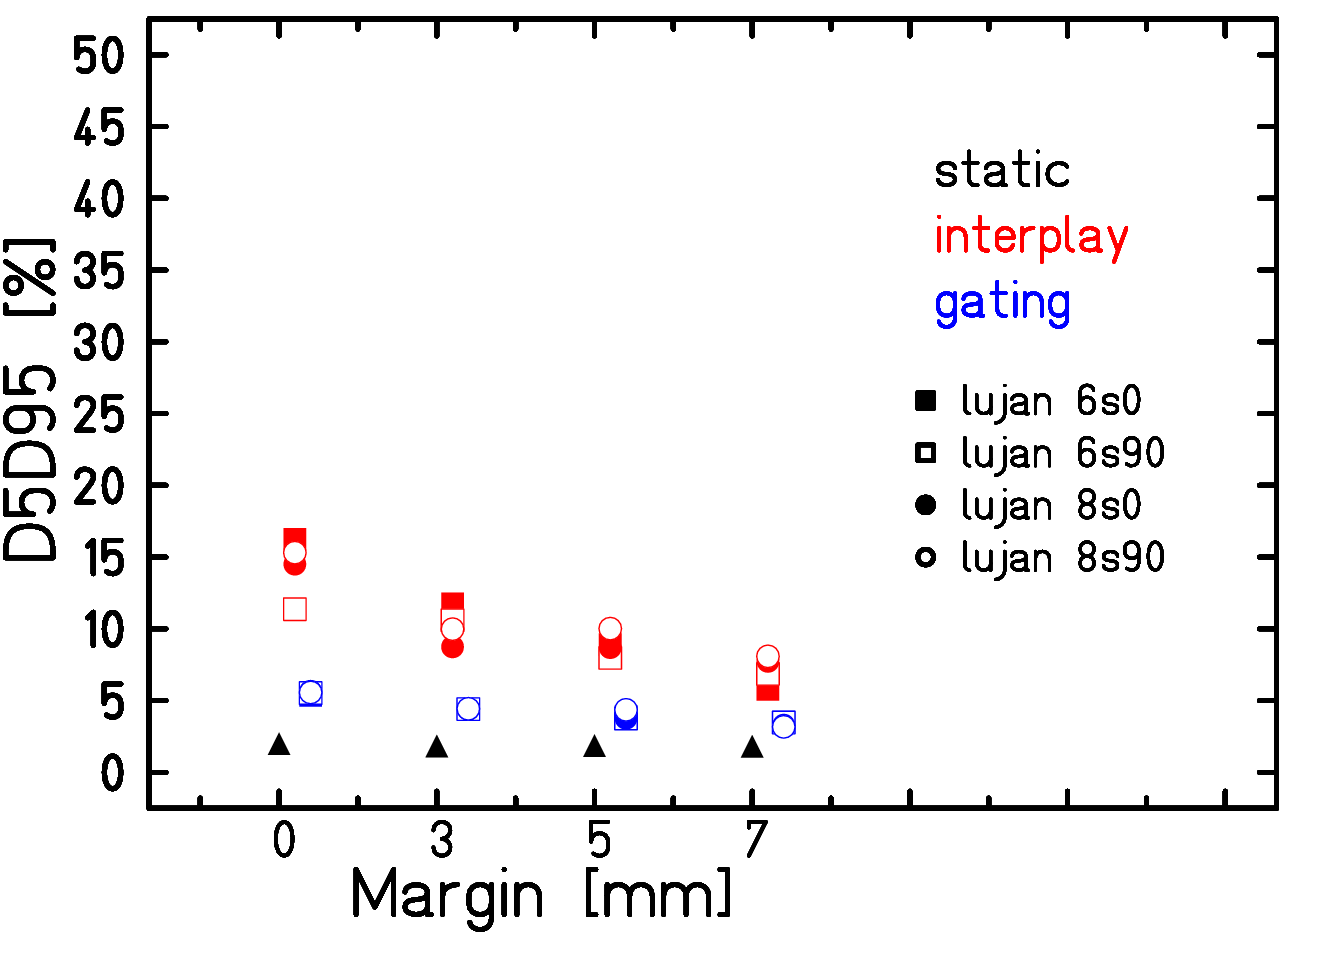
\includegraphics[scale=0.18]{MDACC_Pat023_CTV_LPV_D5D95.png}
 }
 \subfigure[D5-D95: RPV]{
 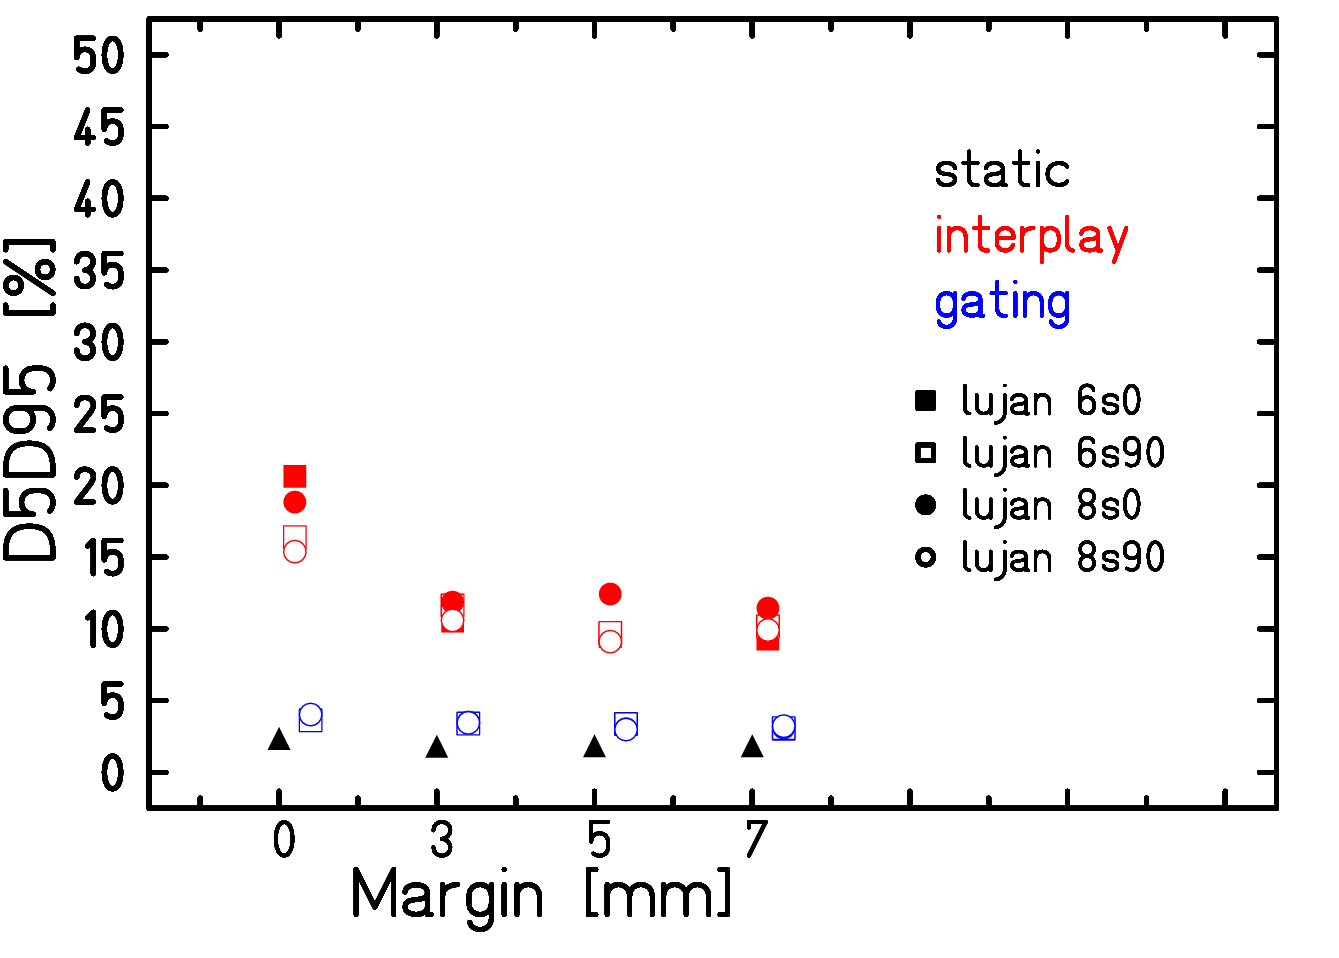
\includegraphics[scale=0.18]{MDACC_Pat023_CTV_RPV_D5D95.png}
 }
 \subfigure[V95: LPV]{
 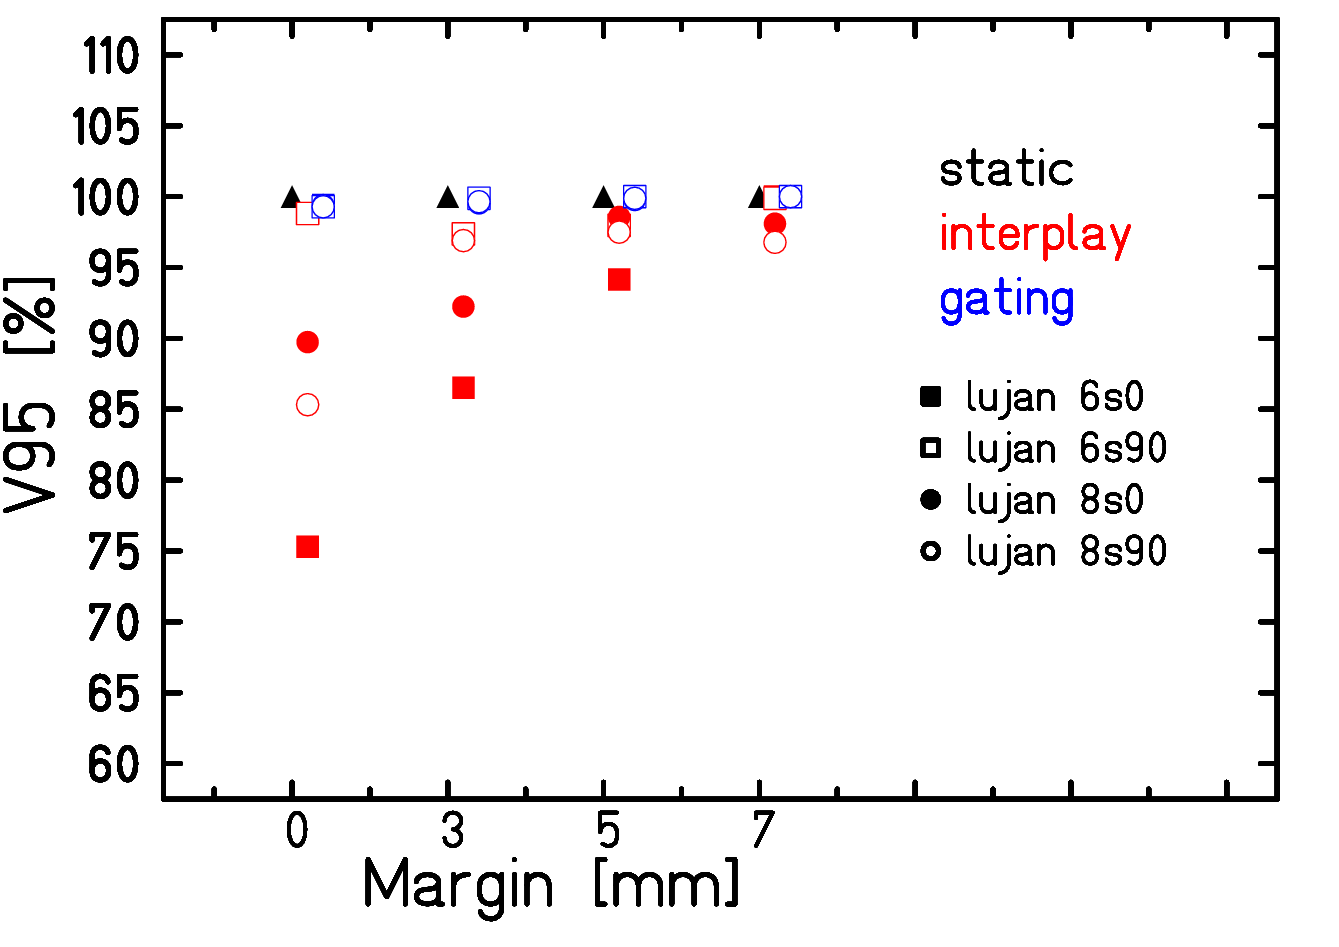
\includegraphics[scale=0.18]{MDACC_Pat023_CTV_LPV_V95.png}
 }
\subfigure[V95: RPV]{
 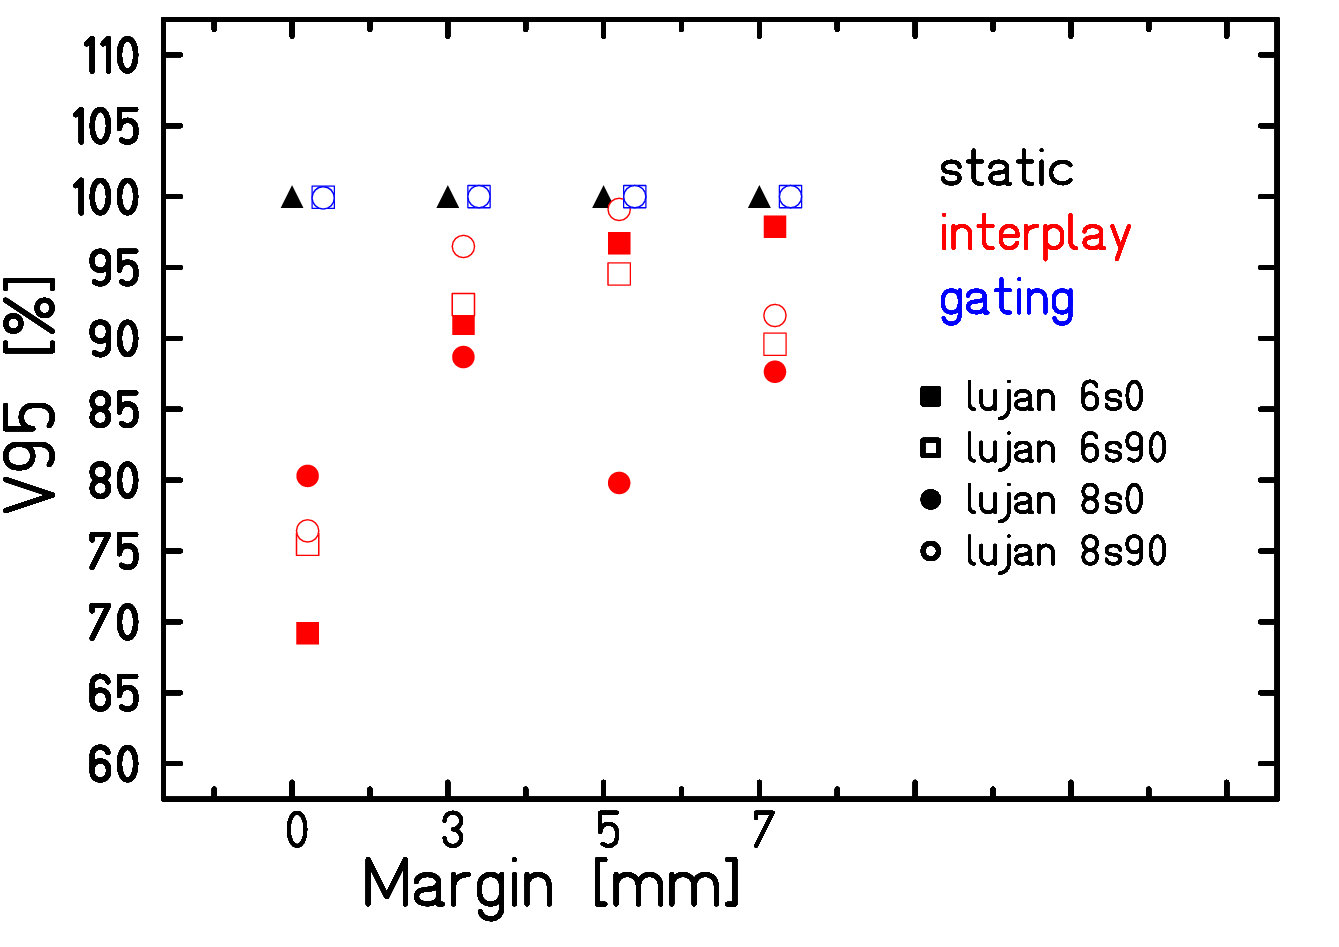
\includegraphics[scale=0.18]{MDACC_Pat023_CTV_RPV_V95.png}
 }
  \subfigure[V107: LPV]{
 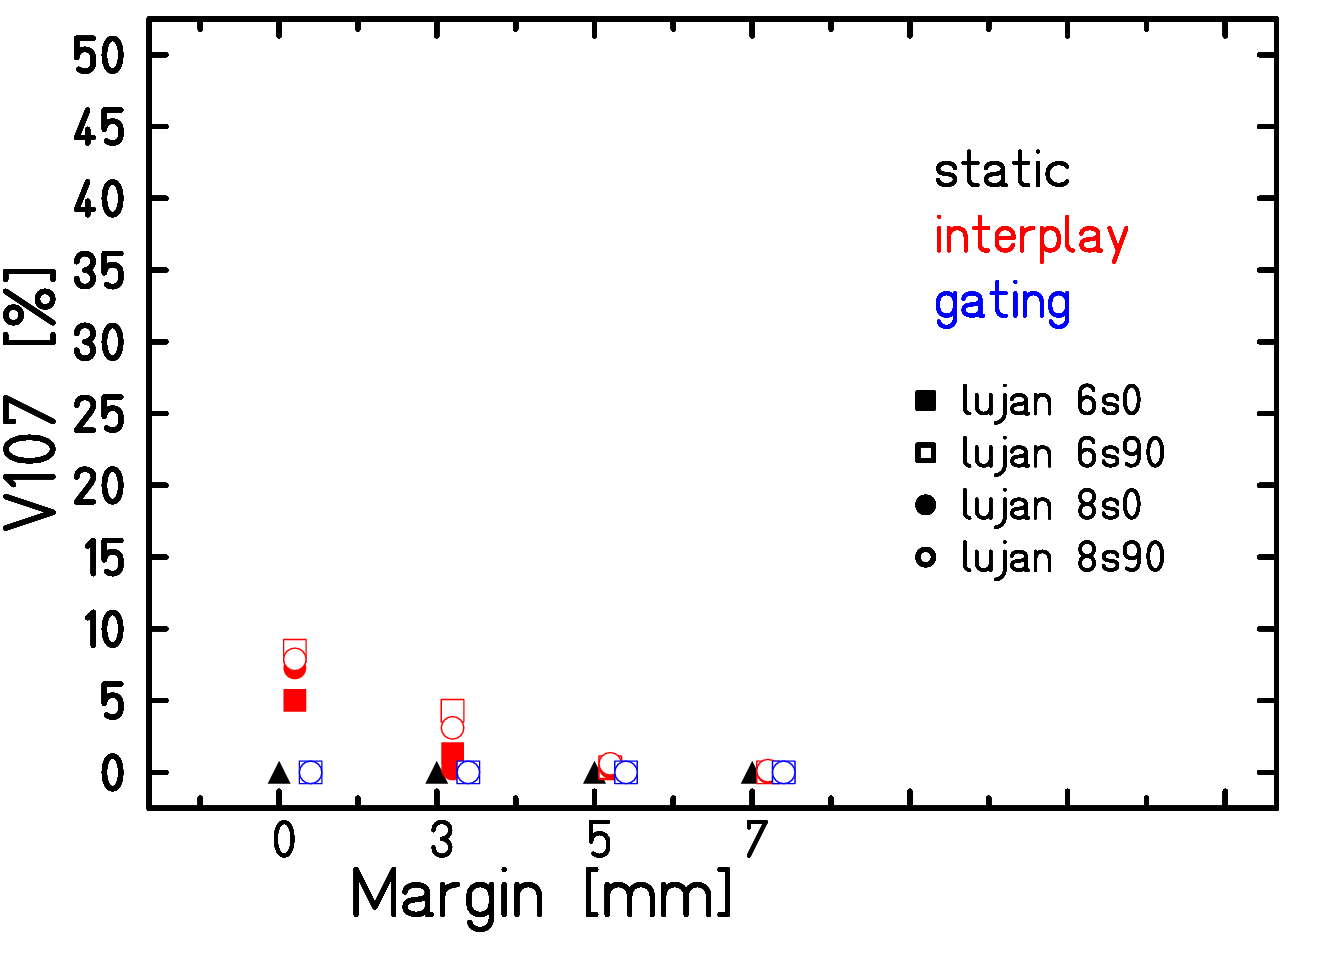
\includegraphics[scale=0.18]{MDACC_Pat023_CTV_LPV_V107.png}
 }
\subfigure[V107: RPV]{
 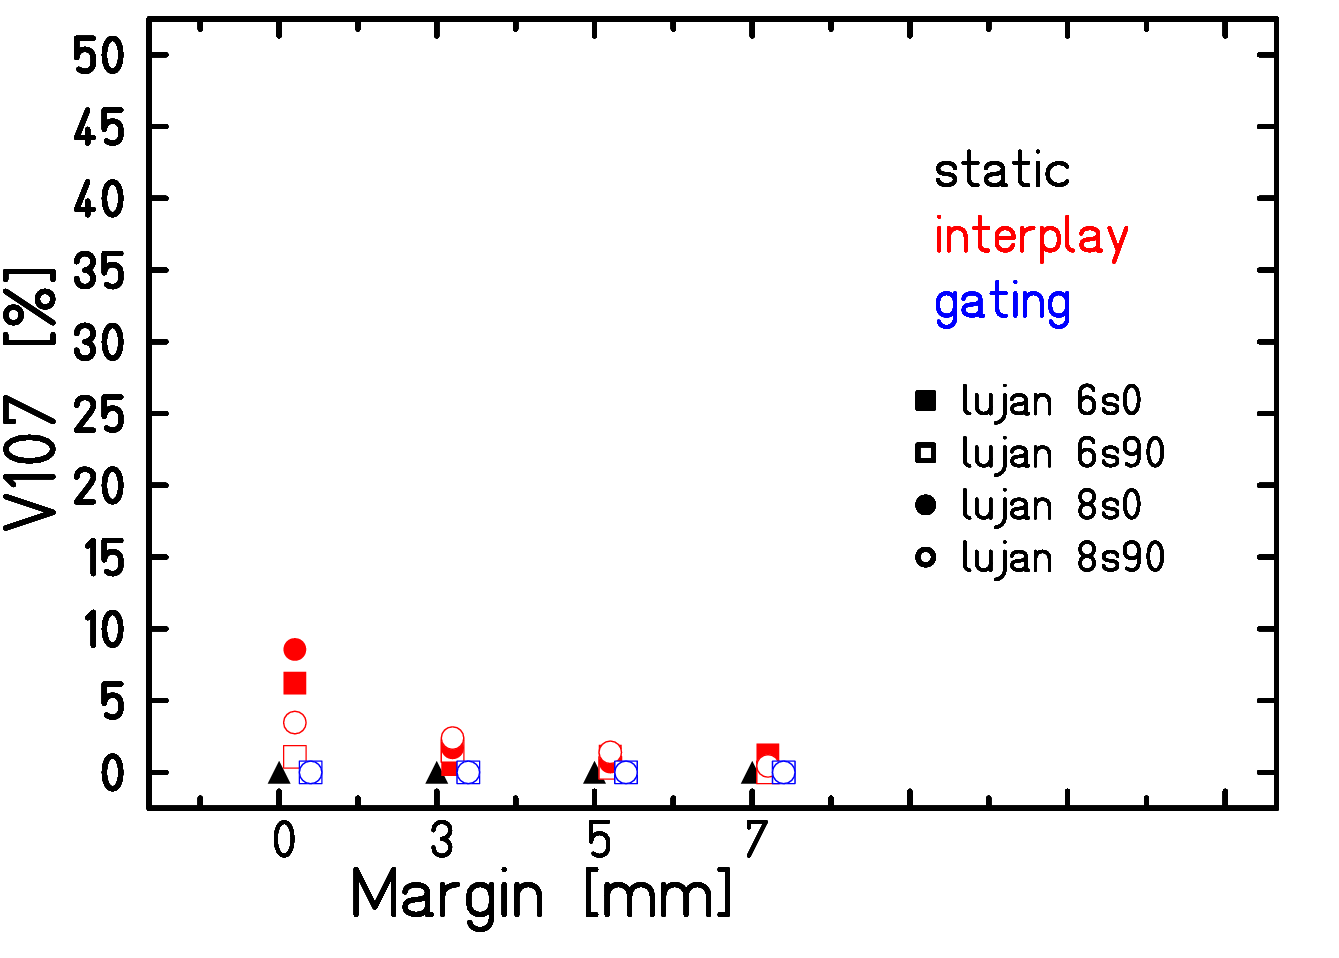
\includegraphics[scale=0.18]{MDACC_Pat023_CTV_RPV_V107.png}
 }
\caption{Patient 1: Dose analysis parameters D5-D95 (dose homogeneity, first row), V95 (dose coverage, middle row) and V107 (over dosage, last row). 
The LPV (left column) and RPV (right column) were studied seperately. Static (black) as well as interplay (red) and gating (blue) 
are compared for four different motions and different safety margins.}
\label{static_interplay_gating_Pat01}
\end{figure}

\begin{figure}[H]
\subfigure[D5-D95: LPV]{
 \includegraphics[scale=0.18]{MDACC_Pat024_CTV_LPV_D5D95.png}
 }
 \subfigure[D5-D95: RPV]{
 \includegraphics[scale=0.18]{MDACC_Pat024_CTV_RPV_D5D95.png}
 }
 \subfigure[V95: LPV]{
 \includegraphics[scale=0.18]{MDACC_Pat024_CTV_LPV_V95.png}
 }
\subfigure[V95: RPV]{
 \includegraphics[scale=0.18]{MDACC_Pat024_CTV_RPV_V95.png}
 }
  \subfigure[V107: LPV]{
 \includegraphics[scale=0.18]{MDACC_Pat024_CTV_LPV_V107.png}
 }
\subfigure[V107: RPV]{
 \includegraphics[scale=0.18]{MDACC_Pat024_CTV_RPV_V107.png}
 }
\caption{Patient 2: Dose analysis parameters D5-D95 (dose homogeneity, first row), V95 (dose coverage, middle row) and V107 (over dosage, last row). 
The LPV (left column) and RPV (right column) were studied seperately. Static (black) as well as interplay (red) and gating (blue) 
are compared for four different motions and different safety margins.}
\label{static_interplay_gating_Pat02}
\end{figure}

\newpage 

\begin{figure}[H]
\subfigure[D5-D95: LPV]{
 \includegraphics[scale=0.18]{MDACC_Pat026_CTV_LPV_D5D95.png}
 }
 \subfigure[D5-D95: RPV]{
 \includegraphics[scale=0.18]{MDACC_Pat026_CTV_RPV_D5D95.png}
 }
 \subfigure[V95: LPV]{
 \includegraphics[scale=0.18]{MDACC_Pat026_CTV_LPV_V95.png}
 }
\subfigure[V95: RPV]{
 \includegraphics[scale=0.18]{MDACC_Pat026_CTV_RPV_V95.png}
 }
  \subfigure[V107: LPV]{
 \includegraphics[scale=0.18]{MDACC_Pat026_CTV_LPV_V107.png}
 }
\subfigure[V107: RPV]{
 \includegraphics[scale=0.18]{MDACC_Pat026_CTV_RPV_V107.png}
 }
\caption{Patient 3: Dose analysis parameters D5-D95 (dose homogeneity, first row), V95 (dose coverage, middle row) and V107 (over dosage, last row). 
The LPV (left column) and RPV (right column) were studied seperately. Static (black) as well as interplay (red) and gating (blue) 
are compared for four different motions and different safety margins.}
\label{static_interplay_gating_Pat03}
\end{figure}

\newpage 

\begin{figure}[H]
\subfigure[D5-D95: LPV]{
 \includegraphics[scale=0.18]{MDACC_Pat031_CTV_LPV_D5D95.png}
 }
 \subfigure[D5-D95: RPV]{
 \includegraphics[scale=0.18]{MDACC_Pat031_CTV_RPV_D5D95.png}
 }
 \subfigure[V95: LPV]{
 \includegraphics[scale=0.18]{MDACC_Pat031_CTV_LPV_V95.png}
 }
\subfigure[V95: RPV]{
 \includegraphics[scale=0.18]{MDACC_Pat031_CTV_RPV_V95.png}
 }
  \subfigure[V107: LPV]{
 \includegraphics[scale=0.18]{MDACC_Pat031_CTV_LPV_V107.png}
 }
\subfigure[V107: RPV]{
 \includegraphics[scale=0.18]{MDACC_Pat031_CTV_RPV_V107.png}
 }
\caption{Patient 4: Dose analysis parameters D5-D95 (dose homogeneity, first row), V95 (dose coverage, middle row) and V107 (over dosage, last row). 
The LPV (left column) and RPV (right column) were studied seperately. Static (black) as well as interplay (red) and gating (blue) 
are compared for four different motions and different safety margins.}
\label{static_interplay_gating_Pat04}
\end{figure}

\newpage 

\begin{figure}[H]
\subfigure[D5-D95: LPV]{
 \includegraphics[scale=0.18]{MDACC_Pat035_CTV_LPV_D5D95.png}
 }
 \subfigure[D5-D95: RPV]{
 \includegraphics[scale=0.18]{MDACC_Pat035_CTV_RPV_D5D95.png}
 }
 \subfigure[V95: LPV]{
 \includegraphics[scale=0.18]{MDACC_Pat035_CTV_LPV_V95.png}
 }
\subfigure[V95: RPV]{
 \includegraphics[scale=0.18]{MDACC_Pat035_CTV_RPV_V95.png}
 }
  \subfigure[V107: LPV]{
 \includegraphics[scale=0.18]{MDACC_Pat035_CTV_LPV_V107.png}
 }
\subfigure[V107: RPV]{
 \includegraphics[scale=0.18]{MDACC_Pat035_CTV_RPV_V107.png}
 }
\caption{Patient 5: Dose analysis parameters D5-D95 (dose homogeneity, first row), V95 (dose coverage, middle row) and V107 (over dosage, last row). 
The LPV (left column) and RPV (right column) were studied seperately. Static (black) as well as interplay (red) and gating (blue) 
are compared for four different motions and different safety margins.}
\label{static_interplay_gating_Pat05}
\end{figure}

\newpage

\begin{figure}[H]
\subfigure[D5-D95: LPV]{
 \includegraphics[scale=0.18]{MDACC_Pat036_CTV_LPV_D5D95.png}
 }
 \subfigure[D5-D95: RPV]{
 \includegraphics[scale=0.18]{MDACC_Pat036_CTV_RPV_D5D95.png}
 }
 \subfigure[V95: LPV]{
 \includegraphics[scale=0.18]{MDACC_Pat036_CTV_LPV_V95.png}
 }
\subfigure[V95: RPV]{
 \includegraphics[scale=0.18]{MDACC_Pat036_CTV_RPV_V95.png}
 }
  \subfigure[V107: LPV]{
 \includegraphics[scale=0.18]{MDACC_Pat036_CTV_LPV_V107.png}
 }
\subfigure[V107: RPV]{
 \includegraphics[scale=0.18]{MDACC_Pat036_CTV_RPV_V107.png}
 }
\caption{Patient 6: Dose analysis parameters D5-D95 (dose homogeneity, first row), V95 (dose coverage, middle row) and V107 (over dosage, last row). 
The LPV (left column) and RPV (right column) were studied seperately. Static (black) as well as interplay (red) and gating (blue) 
are compared for four different motions and different safety margins.}
\label{static_interplay_gating_Pat06}
\end{figure}

\newpage

\begin{figure}[H]
\subfigure[D5-D95: LPV]{
 \includegraphics[scale=0.18]{MDACC_Pat037_CTV_LPV_D5D95.png}
 }
 \subfigure[D5-D95: RPV]{
 \includegraphics[scale=0.18]{MDACC_Pat037_CTV_RPV_D5D95.png}
 }
 \subfigure[V95: LPV]{
 \includegraphics[scale=0.18]{MDACC_Pat037_CTV_LPV_V95.png}
 }
\subfigure[V95: RPV]{
 \includegraphics[scale=0.18]{MDACC_Pat037_CTV_RPV_V95.png}
 }
  \subfigure[V107: LPV]{
 \includegraphics[scale=0.18]{MDACC_Pat037_CTV_LPV_V107.png}
 }
\subfigure[V107: RPV]{
 \includegraphics[scale=0.18]{MDACC_Pat037_CTV_RPV_V107.png}
 }
\caption{Patient 7: Dose analysis parameters D5-D95 (dose homogeneity, first row), V95 (dose coverage, middle row) and V107 (over dosage, last row). 
The LPV (left column) and RPV (right column) were studied seperately. Static (black) as well as interplay (red) and gating (blue) 
are compared for four different motions and different safety margins.}
\label{static_interplay_gating_Pat07}
\end{figure}

\newpage

\begin{figure}[H]
\subfigure[D5-D95: LPV]{
 \includegraphics[scale=0.18]{MDACC_Pat039_CTV_LPV_D5D95.png}
 }
 \subfigure[D5-D95: RPV]{
 \includegraphics[scale=0.18]{MDACC_Pat039_CTV_RPV_D5D95.png}
 }
 \subfigure[V95: LPV]{
 \includegraphics[scale=0.18]{MDACC_Pat039_CTV_LPV_V95.png}
 }
\subfigure[V95: RPV]{
 \includegraphics[scale=0.18]{MDACC_Pat039_CTV_RPV_V95.png}
 }
  \subfigure[V107: LPV]{
 \includegraphics[scale=0.18]{MDACC_Pat039_CTV_LPV_V107.png}
 }
\subfigure[V107: RPV]{
 \includegraphics[scale=0.18]{MDACC_Pat039_CTV_RPV_V107.png}
 }
\caption{Patient 8: Dose analysis parameters D5-D95 (dose homogeneity, first row), V95 (dose coverage, middle row) and V107 (over dosage, last row). 
The LPV (left column) and RPV (right column) were studied seperately. Static (black) as well as interplay (red) and gating (blue) 
are compared for four different motions and different safety margins.}
\label{static_interplay_gating_Pat08}
\end{figure}

\newpage


\begin{figure}[H]
\subfigure[D5-D95: LPV]{
 \includegraphics[scale=0.18]{MDACC_Pat122_CTV_LPV_D5D95.png}
 }
 \subfigure[D5-D95: RPV]{
 \includegraphics[scale=0.18]{MDACC_Pat122_CTV_RPV_D5D95.png}
 }
 \subfigure[V95: LPV]{
 \includegraphics[scale=0.18]{MDACC_Pat122_CTV_LPV_V95.png}
 }
\subfigure[V95: RPV]{
 \includegraphics[scale=0.18]{MDACC_Pat122_CTV_RPV_V95.png}
 }
  \subfigure[V107: LPV]{
 \includegraphics[scale=0.18]{MDACC_Pat122_CTV_LPV_V107.png}
 }
\subfigure[V107: RPV]{
 \includegraphics[scale=0.18]{MDACC_Pat122_CTV_RPV_V107.png}
 }
\caption{Patient 9: Dose analysis parameters D5-D95 (dose homogeneity, first row), V95 (dose coverage, middle row) and V107 (over dosage, last row). 
The LPV (left column) and RPV (right column) were studied seperately. Static (black) as well as interplay (red) and gating (blue) 
are compared for four different motions and different safety margins.}
\label{static_interplay_gating_Pat09}
\end{figure}


\newpage



\begin{table}[H]
  \centering
  \caption{Patient 1, LPV}
  \begin{tabular}{|c||c|c|c||c|c|c|}
    \hline\hline
    Case & motion period & motion starting phase & Margin & D5-D95 & V95 & V107\\
    \hline 
STATIC & - & - & 0mm & 2.00 & 100.00 & 0.00 \\
STATIC & - & - & 3mm & 1.83 & 100.00 & 0.00 \\
STATIC & - & - & 5mm & 1.86 & 100.00 & 0.00 \\
STATIC & - & - & 7mm & 1.82 & 100.00 & 0.00 \\
INTERPLAY & 6s & 0 & 0mm & 16.23 & 75.30 & 5.01 \\
INTERPLAY & 6s & 90 & 0mm & 11.37 & 98.81 & 8.47 \\
INTERPLAY & 8s & 0 & 0mm & 14.51 & 89.74 & 7.28 \\
INTERPLAY & 8s & 90 & 0mm & 15.31 & 85.32 & 7.88 \\
INTERPLAY & 6s & 0 & 3mm & 11.73 & 86.52 & 1.31 \\
INTERPLAY & 6s & 90 & 3mm & 10.60 & 97.37 & 4.30 \\
INTERPLAY & 8s & 0 & 3mm & 8.75 & 92.24 & 0.24 \\
INTERPLAY & 8s & 90 & 3mm & 9.98 & 96.90 & 3.10 \\
INTERPLAY & 6s & 0 & 5mm & 8.91 & 94.15 & 0.24 \\
INTERPLAY & 6s & 90 & 5mm & 7.98 & 97.97 & 0.36 \\
INTERPLAY & 8s & 0 & 5mm & 8.69 & 98.57 & 0.36 \\
INTERPLAY & 8s & 90 & 5mm & 10.02 & 97.49 & 0.60 \\
INTERPLAY & 6s & 0 & 7mm & 5.79 & 100.00 & 0.00 \\
INTERPLAY & 6s & 90 & 7mm & 6.86 & 99.88 & 0.00 \\
INTERPLAY & 8s & 0 & 7mm & 7.74 & 98.09 & 0.00 \\
INTERPLAY & 8s & 90 & 7mm & 8.09 & 96.78 & 0.12 \\
GATING & 6s & 0 & 0mm & 5.37 & 99.40 & 0.00 \\
GATING & 6s & 90 & 0mm & 5.53 & 99.28 & 0.00 \\
GATING & 8s & 0 & 0mm & 5.65 & 99.40 & 0.00 \\
GATING & 8s & 90 & 0mm & 5.57 & 99.28 & 0.00 \\
GATING & 6s & 0 & 3mm & 4.41 & 99.88 & 0.00 \\
GATING & 6s & 90 & 3mm & 4.41 & 99.88 & 0.00 \\
GATING & 8s & 0 & 3mm & 4.39 & 99.52 & 0.00 \\
GATING & 8s & 90 & 3mm & 4.43 & 99.64 & 0.00 \\
GATING & 6s & 0 & 5mm & 3.88 & 100.00 & 0.00 \\
GATING & 6s & 90 & 5mm & 3.76 & 100.00 & 0.00 \\
GATING & 8s & 0 & 5mm & 3.77 & 99.76 & 0.00 \\
GATING & 8s & 90 & 5mm & 4.36 & 99.88 & 0.00 \\
GATING & 6s & 0 & 7mm & 3.50 & 100.00 & 0.00 \\
GATING & 6s & 90 & 7mm & 3.47 & 100.00 & 0.00 \\
GATING & 8s & 0 & 7mm & 3.29 & 100.00 & 0.00 \\
GATING & 8s & 90 & 7mm & 3.17 & 100.00 & 0.00 \\
    \hline\hline 
  \end{tabular}
\end{table}

\newpage

\begin{table}[H]
  \centering
  \caption{Patient 1, RPV}
  \begin{tabular}{|c||c|c|c||c|c|c|}
    \hline\hline
    Case & motion period & motion starting phase & Margin & D5-D95 & V95 & V107\\
    \hline 
STATIC & - & - & 0mm & 2.36 & 100.00 & 0.00 \\
STATIC & - & - & 3mm & 1.81 & 100.00 & 0.00 \\
STATIC & - & - & 5mm & 1.85 & 100.00 & 0.00 \\
STATIC & - & - & 7mm & 1.84 & 100.00 & 0.00 \\
INTERPLAY & 6s & 0 & 0mm & 20.62 & 69.21 & 6.22 \\
INTERPLAY & 6s & 90 & 0mm & 16.39 & 75.47 & 1.08 \\
INTERPLAY & 8s & 0 & 0mm & 18.83 & 80.30 & 8.57 \\
INTERPLAY & 8s & 90 & 0mm & 15.38 & 76.42 & 3.47 \\
INTERPLAY & 6s & 0 & 3mm & 10.54 & 91.03 & 0.54 \\
INTERPLAY & 6s & 90 & 3mm & 11.63 & 92.38 & 1.49 \\
INTERPLAY & 8s & 0 & 3mm & 11.86 & 88.68 & 1.71 \\
INTERPLAY & 8s & 90 & 3mm & 10.59 & 96.48 & 2.39 \\
INTERPLAY & 6s & 0 & 5mm & 9.46 & 96.71 & 1.13 \\
INTERPLAY & 6s & 90 & 5mm & 9.72 & 94.54 & 0.32 \\
INTERPLAY & 8s & 0 & 5mm & 12.43 & 79.80 & 0.72 \\
INTERPLAY & 8s & 90 & 5mm & 9.11 & 99.10 & 1.40 \\
INTERPLAY & 6s & 0 & 7mm & 9.29 & 97.88 & 1.22 \\
INTERPLAY & 6s & 90 & 7mm & 10.18 & 89.59 & 0.00 \\
INTERPLAY & 8s & 0 & 7mm & 11.44 & 87.65 & 0.50 \\
INTERPLAY & 8s & 90 & 7mm & 9.92 & 91.61 & 0.45 \\
GATING & 6s & 0 & 0mm & 3.62 & 99.95 & 0.00 \\
GATING & 6s & 90 & 0mm & 3.63 & 99.95 & 0.00 \\
GATING & 8s & 0 & 0mm & 4.02 & 99.95 & 0.00 \\
GATING & 8s & 90 & 0mm & 4.03 & 99.91 & 0.00 \\
GATING & 6s & 0 & 3mm & 3.40 & 100.00 & 0.00 \\
GATING & 6s & 90 & 3mm & 3.40 & 100.00 & 0.00 \\
GATING & 8s & 0 & 3mm & 3.51 & 100.00 & 0.00 \\
GATING & 8s & 90 & 3mm & 3.45 & 100.00 & 0.00 \\
GATING & 6s & 0 & 5mm & 3.40 & 100.00 & 0.00 \\
GATING & 6s & 90 & 5mm & 3.37 & 100.00 & 0.00 \\
GATING & 8s & 0 & 5mm & 3.04 & 100.00 & 0.00 \\
GATING & 8s & 90 & 5mm & 2.98 & 100.00 & 0.00 \\
GATING & 6s & 0 & 7mm & 3.00 & 100.00 & 0.00 \\
GATING & 6s & 90 & 7mm & 3.08 & 100.00 & 0.00 \\
GATING & 8s & 0 & 7mm & 3.09 & 100.00 & 0.00 \\
GATING & 8s & 90 & 7mm & 3.22 & 100.00 & 0.00 \\
    \hline\hline 
  \end{tabular}
\end{table}

\newpage

\begin{table}[H]
  \centering
  \caption{Patient 2, LPV}
  \begin{tabular}{|c||c|c|c||c|c|c|}
    \hline\hline
    Case & motion period & motion starting phase & Margin & D5-D95 & V95 & V107\\
    \hline 
STATIC & - & - & 0mm & 1.89 & 100.00 & 0.00 \\
STATIC & - & - & 3mm & 1.85 & 100.00 & 0.00 \\
STATIC & - & - & 5mm & 1.85 & 100.00 & 0.00 \\
STATIC & - & - & 7mm & 1.86 & 100.00 & 0.00 \\
INTERPLAY & 6s & 0 & 0mm & 10.82 & 92.42 & 1.37 \\
INTERPLAY & 6s & 90 & 0mm & 10.68 & 94.97 & 2.35 \\
INTERPLAY & 8s & 0 & 0mm & 8.70 & 97.78 & 1.31 \\
INTERPLAY & 8s & 90 & 0mm & 8.56 & 96.54 & 1.31 \\
INTERPLAY & 6s & 0 & 3mm & 8.38 & 98.82 & 0.07 \\
INTERPLAY & 6s & 90 & 3mm & 8.41 & 98.63 & 0.33 \\
INTERPLAY & 8s & 0 & 3mm & 6.98 & 99.41 & 0.00 \\
INTERPLAY & 8s & 90 & 3mm & 7.77 & 98.76 & 1.11 \\
INTERPLAY & 6s & 0 & 5mm & 7.34 & 97.71 & 0.13 \\
INTERPLAY & 6s & 90 & 5mm & 7.15 & 99.28 & 0.00 \\
INTERPLAY & 8s & 0 & 5mm & 7.20 & 100.00 & 0.13 \\
INTERPLAY & 8s & 90 & 5mm & 7.32 & 98.69 & 0.00 \\
INTERPLAY & 6s & 0 & 7mm & 6.07 & 99.87 & 0.00 \\
INTERPLAY & 6s & 90 & 7mm & 7.01 & 99.48 & 0.20 \\
INTERPLAY & 8s & 0 & 7mm & 6.40 & 99.48 & 0.00 \\
INTERPLAY & 8s & 90 & 7mm & 6.44 & 99.08 & 0.00 \\
GATING & 6s & 0 & 0mm & 6.96 & 99.41 & 0.13 \\
GATING & 6s & 90 & 0mm & 6.93 & 99.28 & 0.00 \\
GATING & 8s & 0 & 0mm & 6.71 & 99.87 & 0.00 \\
GATING & 8s & 90 & 0mm & 7.12 & 99.67 & 0.00 \\
GATING & 6s & 0 & 3mm & 6.81 & 98.43 & 0.07 \\
GATING & 6s & 90 & 3mm & 6.79 & 98.37 & 0.07 \\
GATING & 8s & 0 & 3mm & 4.94 & 99.93 & 0.00 \\
GATING & 8s & 90 & 3mm & 5.10 & 99.93 & 0.00 \\
GATING & 6s & 0 & 5mm & 5.27 & 100.00 & 0.00 \\
GATING & 6s & 90 & 5mm & 4.98 & 99.93 & 0.00 \\
GATING & 8s & 0 & 5mm & 5.39 & 99.41 & 0.00 \\
GATING & 8s & 90 & 5mm & 5.54 & 99.22 & 0.00 \\
GATING & 6s & 0 & 7mm & 4.60 & 100.00 & 0.00 \\
GATING & 6s & 90 & 7mm & 4.53 & 100.00 & 0.00 \\
GATING & 8s & 0 & 7mm & 4.89 & 100.00 & 0.00 \\
GATING & 8s & 90 & 7mm & 4.30 & 100.00 & 0.00 \\
    \hline\hline 
  \end{tabular}
\end{table}

\newpage

\begin{table}[H]
  \centering
  \caption{Patient 2, RPV}
  \begin{tabular}{|c||c|c|c||c|c|c|}
    \hline\hline
    Case & motion period & motion starting phase & Margin & D5-D95 & V95 & V107\\
    \hline 
STATIC & - & - & 0mm & 1.85 & 100.00 & 0.00 \\
STATIC & - & - & 3mm & 1.82 & 100.00 & 0.00 \\
STATIC & - & - & 5mm & 1.84 & 100.00 & 0.00 \\
STATIC & - & - & 7mm & 1.81 & 100.00 & 0.00 \\
INTERPLAY & 6s & 0 & 0mm & 10.03 & 98.51 & 3.32 \\
INTERPLAY & 6s & 90 & 0mm & 9.87 & 97.52 & 1.78 \\
INTERPLAY & 8s & 0 & 0mm & 9.31 & 96.53 & 0.74 \\
INTERPLAY & 8s & 90 & 0mm & 10.27 & 96.14 & 1.44 \\
INTERPLAY & 6s & 0 & 3mm & 6.64 & 97.92 & 0.00 \\
INTERPLAY & 6s & 90 & 3mm & 7.38 & 99.01 & 0.00 \\
INTERPLAY & 8s & 0 & 3mm & 7.43 & 96.53 & 0.00 \\
INTERPLAY & 8s & 90 & 3mm & 7.67 & 95.84 & 0.00 \\
INTERPLAY & 6s & 0 & 5mm & 8.73 & 97.77 & 0.64 \\
INTERPLAY & 6s & 90 & 5mm & 8.84 & 96.73 & 0.64 \\
INTERPLAY & 8s & 0 & 5mm & 7.29 & 98.47 & 0.20 \\
INTERPLAY & 8s & 90 & 5mm & 7.80 & 99.50 & 0.20 \\
INTERPLAY & 6s & 0 & 7mm & 6.61 & 98.61 & 0.00 \\
INTERPLAY & 6s & 90 & 7mm & 7.38 & 98.07 & 0.00 \\
INTERPLAY & 8s & 0 & 7mm & 7.01 & 99.01 & 0.00 \\
INTERPLAY & 8s & 90 & 7mm & 7.53 & 97.77 & 1.24 \\
GATING & 6s & 0 & 0mm & 6.04 & 97.57 & 0.00 \\
GATING & 6s & 90 & 0mm & 6.02 & 98.07 & 0.00 \\
GATING & 8s & 0 & 0mm & 6.32 & 98.17 & 0.00 \\
GATING & 8s & 90 & 0mm & 6.19 & 98.27 & 0.00 \\
GATING & 6s & 0 & 3mm & 4.87 & 99.01 & 0.00 \\
GATING & 6s & 90 & 3mm & 4.95 & 99.70 & 0.00 \\
GATING & 8s & 0 & 3mm & 4.27 & 99.90 & 0.00 \\
GATING & 8s & 90 & 3mm & 4.37 & 99.75 & 0.00 \\
GATING & 6s & 0 & 5mm & 4.26 & 100.00 & 0.00 \\
GATING & 6s & 90 & 5mm & 4.05 & 100.00 & 0.00 \\
GATING & 8s & 0 & 5mm & 4.28 & 99.95 & 0.00 \\
GATING & 8s & 90 & 5mm & 3.92 & 99.95 & 0.10 \\
GATING & 6s & 0 & 7mm & 3.70 & 100.00 & 0.00 \\
GATING & 6s & 90 & 7mm & 3.73 & 100.00 & 0.00 \\
GATING & 8s & 0 & 7mm & 3.81 & 99.95 & 0.00 \\
GATING & 8s & 90 & 7mm & 3.81 & 99.85 & 0.00 \\
    \hline\hline 
  \end{tabular}
\end{table}

\newpage

\begin{table}[H]
  \centering
  \caption{Patient 3, LPV}
  \begin{tabular}{|c||c|c|c||c|c|c|}
    \hline\hline
    Case & motion period & motion starting phase & Margin & D5-D95 & V95 & V107\\
    \hline 
STATIC & - & - & 0mm & 2.24 & 100.00 & 0.00 \\
STATIC & - & - & 3mm & 1.84 & 100.00 & 0.00 \\
STATIC & - & - & 5mm & 1.82 & 100.00 & 0.00 \\
STATIC & - & - & 7mm & 1.82 & 100.00 & 0.00 \\
INTERPLAY & 6s & 0 & 0mm & 15.27 & 89.72 & 8.00 \\
INTERPLAY & 6s & 90 & 0mm & 13.25 & 89.24 & 4.35 \\
INTERPLAY & 8s & 0 & 0mm & 15.22 & 88.98 & 7.56 \\
INTERPLAY & 8s & 90 & 0mm & 13.31 & 88.72 & 3.80 \\
INTERPLAY & 6s & 0 & 3mm & 10.89 & 93.14 & 1.51 \\
INTERPLAY & 6s & 90 & 3mm & 11.06 & 90.93 & 1.36 \\
INTERPLAY & 8s & 0 & 3mm & 10.35 & 96.06 & 1.22 \\
INTERPLAY & 8s & 90 & 3mm & 11.36 & 93.25 & 1.58 \\
INTERPLAY & 6s & 0 & 5mm & 11.44 & 89.50 & 1.14 \\
INTERPLAY & 6s & 90 & 5mm & 10.98 & 96.83 & 3.83 \\
INTERPLAY & 8s & 0 & 5mm & 10.54 & 92.41 & 0.63 \\
INTERPLAY & 8s & 90 & 5mm & 10.86 & 94.36 & 2.73 \\
INTERPLAY & 6s & 0 & 7mm & 9.75 & 97.09 & 1.58 \\
INTERPLAY & 6s & 90 & 7mm & 8.92 & 96.31 & 0.55 \\
INTERPLAY & 8s & 0 & 7mm & 10.81 & 98.45 & 4.50 \\
INTERPLAY & 8s & 90 & 7mm & 11.06 & 94.25 & 2.43 \\
GATING & 6s & 0 & 0mm & 7.09 & 99.04 & 0.22 \\
GATING & 6s & 90 & 0mm & 7.45 & 98.93 & 0.18 \\
GATING & 8s & 0 & 0mm & 7.53 & 98.16 & 0.44 \\
GATING & 8s & 90 & 0mm & 8.06 & 96.98 & 0.22 \\
GATING & 6s & 0 & 3mm & 6.43 & 99.93 & 0.00 \\
GATING & 6s & 90 & 3mm & 6.43 & 100.00 & 0.04 \\
GATING & 8s & 0 & 3mm & 6.27 & 99.93 & 0.15 \\
GATING & 8s & 90 & 3mm & 6.27 & 99.85 & 0.15 \\
GATING & 6s & 0 & 5mm & 6.44 & 99.89 & 0.04 \\
GATING & 6s & 90 & 5mm & 6.35 & 99.85 & 0.04 \\
GATING & 8s & 0 & 5mm & 5.82 & 99.71 & 0.00 \\
GATING & 8s & 90 & 5mm & 6.40 & 98.71 & 0.07 \\
GATING & 6s & 0 & 7mm & 5.22 & 99.96 & 0.04 \\
GATING & 6s & 90 & 7mm & 5.16 & 100.00 & 0.00 \\
GATING & 8s & 0 & 7mm & 5.02 & 100.00 & 0.00 \\
GATING & 8s & 90 & 7mm & 5.00 & 100.00 & 0.00 \\
    \hline\hline 
  \end{tabular}
\end{table}

\newpage

\begin{table}[H]
  \centering
  \caption{Patient 3, RPV}
  \begin{tabular}{|c||c|c|c||c|c|c|}
    \hline\hline
    Case & motion period & motion starting phase & Margin & D5-D95 & V95 & V107\\
    \hline 
STATIC & - & - & 0mm & 1.89 & 100.00 & 0.00 \\
STATIC & - & - & 3mm & 1.82 & 100.00 & 0.00 \\
STATIC & - & - & 5mm & 1.81 & 100.00 & 0.00 \\
STATIC & - & - & 7mm & 1.86 & 100.00 & 0.00 \\
INTERPLAY & 6s & 0 & 0mm & 12.34 & 88.95 & 1.01 \\
INTERPLAY & 6s & 90 & 0mm & 12.23 & 91.57 & 3.84 \\
INTERPLAY & 8s & 0 & 0mm & 12.39 & 91.63 & 3.69 \\
INTERPLAY & 8s & 90 & 0mm & 11.66 & 93.24 & 3.05 \\
INTERPLAY & 6s & 0 & 3mm & 9.29 & 95.81 & 0.56 \\
INTERPLAY & 6s & 90 & 3mm & 9.46 & 97.11 & 1.26 \\
INTERPLAY & 8s & 0 & 3mm & 12.20 & 92.64 & 3.05 \\
INTERPLAY & 8s & 90 & 3mm & 12.80 & 92.04 & 5.07 \\
INTERPLAY & 6s & 0 & 5mm & 8.79 & 98.39 & 1.42 \\
INTERPLAY & 6s & 90 & 5mm & 9.26 & 97.42 & 0.91 \\
INTERPLAY & 8s & 0 & 5mm & 10.30 & 97.01 & 1.88 \\
INTERPLAY & 8s & 90 & 5mm & 9.88 & 96.19 & 1.15 \\
INTERPLAY & 6s & 0 & 7mm & 9.31 & 97.32 & 1.09 \\
INTERPLAY & 6s & 90 & 7mm & 8.63 & 98.78 & 0.49 \\
INTERPLAY & 8s & 0 & 7mm & 10.44 & 94.89 & 1.79 \\
INTERPLAY & 8s & 90 & 7mm & 9.97 & 95.98 & 0.72 \\
GATING & 6s & 0 & 0mm & 5.00 & 99.86 & 0.00 \\
GATING & 6s & 90 & 0mm & 5.02 & 99.86 & 0.00 \\
GATING & 8s & 0 & 0mm & 5.31 & 99.86 & 0.00 \\
GATING & 8s & 90 & 0mm & 5.57 & 99.77 & 0.06 \\
GATING & 6s & 0 & 3mm & 4.49 & 100.00 & 0.00 \\
GATING & 6s & 90 & 3mm & 4.58 & 100.00 & 0.00 \\
GATING & 8s & 0 & 3mm & 4.49 & 100.00 & 0.06 \\
GATING & 8s & 90 & 3mm & 4.88 & 100.00 & 0.02 \\
GATING & 6s & 0 & 5mm & 4.94 & 100.00 & 0.00 \\
GATING & 6s & 90 & 5mm & 4.89 & 100.00 & 0.00 \\
GATING & 8s & 0 & 5mm & 4.45 & 100.00 & 0.00 \\
GATING & 8s & 90 & 5mm & 4.29 & 100.00 & 0.00 \\
GATING & 6s & 0 & 7mm & 4.08 & 100.00 & 0.00 \\
GATING & 6s & 90 & 7mm & 3.89 & 100.00 & 0.00 \\
GATING & 8s & 0 & 7mm & 3.85 & 99.98 & 0.00 \\
GATING & 8s & 90 & 7mm & 3.84 & 100.00 & 0.00 \\
    \hline\hline 
  \end{tabular}
\end{table}


\newpage

\begin{table}[H]
  \centering
  \caption{Patient 4, LPV}
  \begin{tabular}{|c||c|c|c||c|c|c|}
    \hline\hline
    Case & motion period & motion starting phase & Margin & D5-D95 & V95 & V107\\
    \hline 
STATIC & - & - & 0mm & 1.90 & 100.00 & 0.00 \\
STATIC & - & - & 3mm & 1.83 & 100.00 & 0.00 \\
STATIC & - & - & 5mm & 1.87 & 100.00 & 0.00 \\
STATIC & - & - & 7mm & 1.82 & 100.00 & 0.00 \\
INTERPLAY & 6s & 0 & 0mm & 11.02 & 93.01 & 1.20 \\
INTERPLAY & 6s & 90 & 0mm & 10.34 & 93.08 & 1.13 \\
INTERPLAY & 8s & 0 & 0mm & 16.87 & 84.43 & 7.32 \\
INTERPLAY & 8s & 90 & 0mm & 14.22 & 85.89 & 4.92 \\
INTERPLAY & 6s & 0 & 3mm & 6.43 & 99.40 & 0.00 \\
INTERPLAY & 6s & 90 & 3mm & 7.46 & 98.74 & 0.07 \\
INTERPLAY & 8s & 0 & 3mm & 11.73 & 90.69 & 2.53 \\
INTERPLAY & 8s & 90 & 3mm & 12.31 & 85.43 & 0.86 \\
INTERPLAY & 6s & 0 & 5mm & 6.66 & 98.20 & 0.00 \\
INTERPLAY & 6s & 90 & 5mm & 7.47 & 98.94 & 0.00 \\
INTERPLAY & 8s & 0 & 5mm & 9.12 & 96.67 & 0.73 \\
INTERPLAY & 8s & 90 & 5mm & 9.91 & 94.48 & 0.47 \\
INTERPLAY & 6s & 0 & 7mm & 6.21 & 97.94 & 0.00 \\
INTERPLAY & 6s & 90 & 7mm & 7.09 & 98.60 & 0.00 \\
INTERPLAY & 8s & 0 & 7mm & 7.18 & 98.14 & 0.00 \\
INTERPLAY & 8s & 90 & 7mm & 6.74 & 99.53 & 0.60 \\
GATING & 6s & 0 & 0mm & 3.89 & 99.93 & 0.00 \\
GATING & 6s & 90 & 0mm & 3.81 & 99.93 & 0.00 \\
GATING & 8s & 0 & 0mm & 3.94 & 99.93 & 0.00 \\
GATING & 8s & 90 & 0mm & 4.48 & 99.87 & 0.00 \\
GATING & 6s & 0 & 3mm & 2.87 & 100.00 & 0.00 \\
GATING & 6s & 90 & 3mm & 2.88 & 100.00 & 0.00 \\
GATING & 8s & 0 & 3mm & 3.20 & 100.00 & 0.00 \\
GATING & 8s & 90 & 3mm & 3.10 & 100.00 & 0.00 \\
GATING & 6s & 0 & 5mm & 2.90 & 100.00 & 0.00 \\
GATING & 6s & 90 & 5mm & 3.03 & 100.00 & 0.00 \\
GATING & 8s & 0 & 5mm & 2.94 & 100.00 & 0.00 \\
GATING & 8s & 90 & 5mm & 3.13 & 100.00 & 0.00 \\
GATING & 6s & 0 & 7mm & 2.99 & 100.00 & 0.00 \\
GATING & 6s & 90 & 7mm & 3.01 & 100.00 & 0.00 \\
GATING & 8s & 0 & 7mm & 2.88 & 100.00 & 0.00 \\
GATING & 8s & 90 & 7mm & 2.83 & 100.00 & 0.00 \\
    \hline\hline 
  \end{tabular}
\end{table}

\newpage

\begin{table}[H]
  \centering
  \caption{Patient 4, RPV}
  \begin{tabular}{|c||c|c|c||c|c|c|}
    \hline\hline
    Case & motion period & motion starting phase & Margin & D5-D95 & V95 & V107\\
    \hline 
STATIC & - & - & 0mm & 1.83 & 100.00 & 0.00 \\
STATIC & - & - & 3mm & 1.80 & 100.00 & 0.00 \\
STATIC & - & - & 5mm & 1.80 & 100.00 & 0.00 \\
STATIC & - & - & 7mm & 1.80 & 100.00 & 0.00 \\
INTERPLAY & 6s & 0 & 0mm & 12.60 & 89.91 & 1.94 \\
INTERPLAY & 6s & 90 & 0mm & 11.01 & 90.89 & 1.82 \\
INTERPLAY & 8s & 0 & 0mm & 13.99 & 87.18 & 5.29 \\
INTERPLAY & 8s & 90 & 0mm & 13.89 & 86.21 & 3.71 \\
INTERPLAY & 6s & 0 & 3mm & 9.72 & 93.13 & 0.30 \\
INTERPLAY & 6s & 90 & 3mm & 9.21 & 96.60 & 0.61 \\
INTERPLAY & 8s & 0 & 3mm & 10.68 & 91.92 & 1.46 \\
INTERPLAY & 8s & 90 & 3mm & 11.23 & 91.07 & 1.52 \\
INTERPLAY & 6s & 0 & 5mm & 9.77 & 95.57 & 0.18 \\
INTERPLAY & 6s & 90 & 5mm & 8.60 & 98.12 & 0.24 \\
INTERPLAY & 8s & 0 & 5mm & 9.75 & 94.47 & 0.43 \\
INTERPLAY & 8s & 90 & 5mm & 9.55 & 97.21 & 1.28 \\
INTERPLAY & 6s & 0 & 7mm & 6.84 & 96.17 & 0.00 \\
INTERPLAY & 6s & 90 & 7mm & 6.25 & 99.70 & 0.00 \\
INTERPLAY & 8s & 0 & 7mm & 8.04 & 98.66 & 0.00 \\
INTERPLAY & 8s & 90 & 7mm & 8.81 & 93.92 & 0.00 \\
GATING & 6s & 0 & 0mm & 4.81 & 100.00 & 0.00 \\
GATING & 6s & 90 & 0mm & 4.86 & 100.00 & 0.00 \\
GATING & 8s & 0 & 0mm & 5.46 & 100.00 & 0.06 \\
GATING & 8s & 90 & 0mm & 5.21 & 99.94 & 0.12 \\
GATING & 6s & 0 & 3mm & 4.04 & 100.00 & 0.00 \\
GATING & 6s & 90 & 3mm & 4.03 & 100.00 & 0.00 \\
GATING & 8s & 0 & 3mm & 4.10 & 100.00 & 0.00 \\
GATING & 8s & 90 & 3mm & 4.26 & 100.00 & 0.00 \\
GATING & 6s & 0 & 5mm & 3.61 & 100.00 & 0.00 \\
GATING & 6s & 90 & 5mm & 3.64 & 100.00 & 0.00 \\
GATING & 8s & 0 & 5mm & 3.59 & 100.00 & 0.00 \\
GATING & 8s & 90 & 5mm & 3.62 & 100.00 & 0.00 \\
GATING & 6s & 0 & 7mm & 2.79 & 100.00 & 0.00 \\
GATING & 6s & 90 & 7mm & 2.81 & 100.00 & 0.00 \\
GATING & 8s & 0 & 7mm & 3.29 & 100.00 & 0.00 \\
GATING & 8s & 90 & 7mm & 3.24 & 100.00 & 0.00 \\
    \hline\hline 
  \end{tabular}
\end{table}


\newpage

\begin{table}[H]
  \centering
  \caption{Patient 5, LPV}
  \begin{tabular}{|c||c|c|c||c|c|c|}
    \hline\hline
    Case & motion period & motion starting phase & Margin & D5-D95 & V95 & V107\\
    \hline  
STATIC & - & - & 0mm & 1.94 & 100.00 & 0.00 \\
STATIC & - & - & 3mm & 1.84 & 100.00 & 0.00 \\
STATIC & - & - & 5mm & 1.83 & 100.00 & 0.00 \\
STATIC & - & - & 7mm & 1.82 & 100.00 & 0.00 \\
INTERPLAY & 6s & 0 & 0mm & 18.21 & 89.36 & 18.18 \\
INTERPLAY & 6s & 90 & 0mm & 14.34 & 88.25 & 5.10 \\
INTERPLAY & 8s & 0 & 0mm & 16.67 & 81.26 & 7.87 \\
INTERPLAY & 8s & 90 & 0mm & 14.40 & 92.13 & 8.98 \\
INTERPLAY & 6s & 0 & 3mm & 14.58 & 89.14 & 6.32 \\
INTERPLAY & 6s & 90 & 3mm & 12.31 & 88.58 & 1.66 \\
INTERPLAY & 8s & 0 & 3mm & 14.69 & 85.92 & 6.98 \\
INTERPLAY & 8s & 90 & 3mm & 14.49 & 90.02 & 6.76 \\
INTERPLAY & 6s & 0 & 5mm & 10.64 & 83.92 & 0.11 \\
INTERPLAY & 6s & 90 & 5mm & 13.25 & 95.57 & 7.76 \\
INTERPLAY & 8s & 0 & 5mm & 14.70 & 92.35 & 14.74 \\
INTERPLAY & 8s & 90 & 5mm & 11.10 & 87.92 & 0.44 \\
INTERPLAY & 6s & 0 & 7mm & 8.34 & 99.89 & 1.44 \\
INTERPLAY & 6s & 90 & 7mm & 7.34 & 96.01 & 0.00 \\
INTERPLAY & 8s & 0 & 7mm & 10.66 & 96.34 & 1.77 \\
INTERPLAY & 8s & 90 & 7mm & 10.14 & 95.57 & 0.22 \\
GATING & 6s & 0 & 0mm & 7.22 & 99.45 & 0.67 \\
GATING & 6s & 90 & 0mm & 7.21 & 99.45 & 0.67 \\
GATING & 8s & 0 & 0mm & 8.88 & 95.23 & 0.33 \\
GATING & 8s & 90 & 0mm & 9.18 & 95.23 & 0.11 \\
GATING & 6s & 0 & 3mm & 6.10 & 98.78 & 0.00 \\
GATING & 6s & 90 & 3mm & 6.16 & 98.56 & 0.11 \\
GATING & 8s & 0 & 3mm & 7.27 & 99.78 & 0.00 \\
GATING & 8s & 90 & 3mm & 7.71 & 99.45 & 0.00 \\
GATING & 6s & 0 & 5mm & 6.81 & 98.45 & 0.00 \\
GATING & 6s & 90 & 5mm & 6.76 & 98.45 & 0.00 \\
GATING & 8s & 0 & 5mm & 7.44 & 97.34 & 0.00 \\
GATING & 8s & 90 & 5mm & 7.25 & 97.56 & 0.00 \\
GATING & 6s & 0 & 7mm & 5.28 & 98.89 & 0.00 \\
GATING & 6s & 90 & 7mm & 5.43 & 99.00 & 0.00 \\
GATING & 8s & 0 & 7mm & 5.60 & 100.00 & 0.00 \\
GATING & 8s & 90 & 7mm & 5.36 & 100.00 & 0.00 \\
    \hline\hline 
  \end{tabular}
\end{table}

\newpage

\begin{table}[H]
  \centering
  \caption{Patient 5, RPV}
  \begin{tabular}{|c||c|c|c||c|c|c|}
    \hline\hline
    Case & motion period & motion starting phase & Margin & D5-D95 & V95 & V107\\
    \hline 
STATIC & - & - & 0mm & 1.85 & 100.00 & 0.00 \\
STATIC & - & - & 3mm & 1.85 & 100.00 & 0.00 \\
STATIC & - & - & 5mm & 1.81 & 100.00 & 0.00 \\
STATIC & - & - & 7mm & 1.81 & 100.00 & 0.00 \\
INTERPLAY & 6s & 0 & 0mm & 12.27 & 95.36 & 6.05 \\
INTERPLAY & 6s & 90 & 0mm & 11.59 & 93.63 & 2.38 \\
INTERPLAY & 8s & 0 & 0mm & 16.30 & 86.88 & 8.91 \\
INTERPLAY & 8s & 90 & 0mm & 12.29 & 94.87 & 5.35 \\
INTERPLAY & 6s & 0 & 3mm & 11.61 & 95.52 & 4.16 \\
INTERPLAY & 6s & 90 & 3mm & 9.22 & 94.98 & 0.92 \\
INTERPLAY & 8s & 0 & 3mm & 12.87 & 87.53 & 2.86 \\
INTERPLAY & 8s & 90 & 3mm & 12.27 & 97.68 & 7.02 \\
INTERPLAY & 6s & 0 & 5mm & 11.58 & 92.98 & 1.46 \\
INTERPLAY & 6s & 90 & 5mm & 11.04 & 95.25 & 2.70 \\
INTERPLAY & 8s & 0 & 5mm & 12.42 & 86.77 & 1.84 \\
INTERPLAY & 8s & 90 & 5mm & 12.55 & 86.45 & 2.05 \\
INTERPLAY & 6s & 0 & 7mm & 9.05 & 99.08 & 0.59 \\
INTERPLAY & 6s & 90 & 7mm & 8.15 & 98.92 & 0.11 \\
INTERPLAY & 8s & 0 & 7mm & 8.60 & 98.11 & 0.65 \\
INTERPLAY & 8s & 90 & 7mm & 8.96 & 98.87 & 1.46 \\
GATING & 6s & 0 & 0mm & 5.79 & 99.89 & 0.00 \\
GATING & 6s & 90 & 0mm & 5.78 & 99.89 & 0.00 \\
GATING & 8s & 0 & 0mm & 5.44 & 99.62 & 0.00 \\
GATING & 8s & 90 & 0mm & 5.38 & 99.68 & 0.00 \\
GATING & 6s & 0 & 3mm & 5.19 & 100.00 & 0.00 \\
GATING & 6s & 90 & 3mm & 5.10 & 100.00 & 0.00 \\
GATING & 8s & 0 & 3mm & 5.99 & 100.00 & 0.00 \\
GATING & 8s & 90 & 3mm & 5.67 & 100.00 & 0.00 \\
GATING & 6s & 0 & 5mm & 4.54 & 99.89 & 0.00 \\
GATING & 6s & 90 & 5mm & 4.57 & 99.95 & 0.00 \\
GATING & 8s & 0 & 5mm & 4.62 & 100.00 & 0.00 \\
GATING & 8s & 90 & 5mm & 4.92 & 100.00 & 0.00 \\
GATING & 6s & 0 & 7mm & 3.86 & 100.00 & 0.00 \\
GATING & 6s & 90 & 7mm & 3.83 & 100.00 & 0.00 \\
GATING & 8s & 0 & 7mm & 4.27 & 100.00 & 0.00 \\
GATING & 8s & 90 & 7mm & 4.68 & 100.00 & 0.00 \\
    \hline\hline 
  \end{tabular}
\end{table}

\newpage

\begin{table}[H]
  \centering
  \caption{Patient 6, LPV}
  \begin{tabular}{|c||c|c|c||c|c|c|}
    \hline\hline
    Case & motion period & motion starting phase & Margin & D5-D95 & V95 & V107\\
    \hline 
STATIC & - & - & 0mm & 1.86 & 100.00 & 0.00 \\
STATIC & - & - & 3mm & 1.84 & 100.00 & 0.00 \\
STATIC & - & - & 5mm & 1.81 & 100.00 & 0.00 \\
STATIC & - & - & 7mm & 1.83 & 100.00 & 0.00 \\
INTERPLAY & 6s & 0 & 0mm & 12.07 & 91.36 & 4.04 \\
INTERPLAY & 6s & 90 & 0mm & 12.94 & 86.83 & 1.13 \\
INTERPLAY & 8s & 0 & 0mm & 17.12 & 75.14 & 5.17 \\
INTERPLAY & 8s & 90 & 0mm & 16.66 & 81.02 & 4.32 \\
INTERPLAY & 6s & 0 & 3mm & 11.39 & 95.25 & 3.54 \\
INTERPLAY & 6s & 90 & 3mm & 8.61 & 96.60 & 0.35 \\
INTERPLAY & 8s & 0 & 3mm & 10.19 & 93.41 & 0.42 \\
INTERPLAY & 8s & 90 & 3mm & 11.22 & 94.41 & 2.62 \\
INTERPLAY & 6s & 0 & 5mm & 8.22 & 97.80 & 0.57 \\
INTERPLAY & 6s & 90 & 5mm & 8.17 & 96.32 & 0.00 \\
INTERPLAY & 8s & 0 & 5mm & 11.32 & 90.37 & 1.20 \\
INTERPLAY & 8s & 90 & 5mm & 10.66 & 92.42 & 1.20 \\
INTERPLAY & 6s & 0 & 7mm & 7.62 & 97.52 & 0.00 \\
INTERPLAY & 6s & 90 & 7mm & 8.20 & 96.88 & 0.14 \\
INTERPLAY & 8s & 0 & 7mm & 9.18 & 92.78 & 0.71 \\
INTERPLAY & 8s & 90 & 7mm & 8.25 & 94.83 & 0.00 \\
GATING & 6s & 0 & 0mm & 7.75 & 96.32 & 0.00 \\
GATING & 6s & 90 & 0mm & 7.83 & 95.96 & 0.00 \\
GATING & 8s & 0 & 0mm & 7.48 & 97.95 & 0.00 \\
GATING & 8s & 90 & 0mm & 7.49 & 98.37 & 0.00 \\
GATING & 6s & 0 & 3mm & 4.92 & 100.00 & 0.00 \\
GATING & 6s & 90 & 3mm & 4.92 & 100.00 & 0.00 \\
GATING & 8s & 0 & 3mm & 5.04 & 100.00 & 0.00 \\
GATING & 8s & 90 & 3mm & 4.63 & 100.00 & 0.00 \\
GATING & 6s & 0 & 5mm & 4.21 & 100.00 & 0.00 \\
GATING & 6s & 90 & 5mm & 4.17 & 100.00 & 0.00 \\
GATING & 8s & 0 & 5mm & 4.34 & 100.00 & 0.00 \\
GATING & 8s & 90 & 5mm & 4.21 & 100.00 & 0.00 \\
GATING & 6s & 0 & 7mm & 4.13 & 100.00 & 0.00 \\
GATING & 6s & 90 & 7mm & 4.12 & 100.00 & 0.00 \\
GATING & 8s & 0 & 7mm & 4.45 & 100.00 & 0.00 \\
GATING & 8s & 90 & 7mm & 4.26 & 100.00 & 0.00 \\
    \hline\hline 
  \end{tabular}
\end{table}

\newpage

\begin{table}[H]
  \centering
  \caption{Patient 6, RPV}
  \begin{tabular}{|c||c|c|c||c|c|c|}
    \hline\hline
    Case & motion period & motion starting phase & Margin & D5-D95 & V95 & V107\\
    \hline 
STATIC & - & - & 0mm & 1.84 & 100.00 & 0.00 \\
STATIC & - & - & 3mm & 1.81 & 100.00 & 0.00 \\
STATIC & - & - & 5mm & 1.81 & 100.00 & 0.00 \\
STATIC & - & - & 7mm & 1.82 & 100.00 & 0.00 \\
INTERPLAY & 6s & 0 & 0mm & 10.31 & 96.14 & 3.00 \\
INTERPLAY & 6s & 90 & 0mm & 10.75 & 91.82 & 0.60 \\
INTERPLAY & 8s & 0 & 0mm & 10.86 & 95.68 & 2.93 \\
INTERPLAY & 8s & 90 & 0mm & 8.92 & 98.27 & 1.31 \\
INTERPLAY & 6s & 0 & 3mm & 10.26 & 98.05 & 3.75 \\
INTERPLAY & 6s & 90 & 3mm & 7.78 & 98.05 & 0.08 \\
INTERPLAY & 8s & 0 & 3mm & 9.51 & 97.07 & 1.73 \\
INTERPLAY & 8s & 90 & 3mm & 8.26 & 98.80 & 0.64 \\
INTERPLAY & 6s & 0 & 5mm & 7.57 & 99.10 & 1.05 \\
INTERPLAY & 6s & 90 & 5mm & 7.80 & 99.44 & 0.83 \\
INTERPLAY & 8s & 0 & 5mm & 8.46 & 95.68 & 0.26 \\
INTERPLAY & 8s & 90 & 5mm & 7.17 & 98.16 & 0.15 \\
INTERPLAY & 6s & 0 & 7mm & 6.83 & 99.77 & 0.00 \\
INTERPLAY & 6s & 90 & 7mm & 8.54 & 99.70 & 2.03 \\
INTERPLAY & 8s & 0 & 7mm & 7.30 & 97.82 & 0.08 \\
INTERPLAY & 8s & 90 & 7mm & 7.45 & 97.07 & 0.08 \\
GATING & 6s & 0 & 0mm & 6.72 & 98.20 & 0.08 \\
GATING & 6s & 90 & 0mm & 6.85 & 98.20 & 0.00 \\
GATING & 8s & 0 & 0mm & 6.47 & 99.59 & 0.04 \\
GATING & 8s & 90 & 0mm & 6.06 & 99.74 & 0.26 \\
GATING & 6s & 0 & 3mm & 5.09 & 100.00 & 0.00 \\
GATING & 6s & 90 & 3mm & 5.23 & 99.96 & 0.00 \\
GATING & 8s & 0 & 3mm & 5.84 & 98.69 & 0.00 \\
GATING & 8s & 90 & 3mm & 5.04 & 99.96 & 0.08 \\
GATING & 6s & 0 & 5mm & 4.57 & 100.00 & 0.00 \\
GATING & 6s & 90 & 5mm & 4.60 & 100.00 & 0.00 \\
GATING & 8s & 0 & 5mm & 4.91 & 100.00 & 0.00 \\
GATING & 8s & 90 & 5mm & 4.87 & 100.00 & 0.04 \\
GATING & 6s & 0 & 7mm & 4.79 & 99.14 & 0.00 \\
GATING & 6s & 90 & 7mm & 4.89 & 99.14 & 0.00 \\
GATING & 8s & 0 & 7mm & 4.03 & 100.00 & 0.00 \\
GATING & 8s & 90 & 7mm & 4.10 & 99.96 & 0.00 \\
    \hline\hline 
  \end{tabular}
\end{table}


\newpage

\begin{table}[H]
  \centering
  \caption{Patient 7, LPV}
  \begin{tabular}{|c||c|c|c||c|c|c|}
    \hline\hline
    Case & motion period & motion starting phase & Margin & D5-D95 & V95 & V107\\
    \hline 
STATIC & - & - & 0mm & 1.94 & 100.00 & 0.00 \\
STATIC & - & - & 3mm & 1.91 & 100.00 & 0.00 \\
STATIC & - & - & 5mm & 1.82 & 100.00 & 0.00 \\
STATIC & - & - & 7mm & 1.83 & 100.00 & 0.00 \\
INTERPLAY & 6s & 0 & 0mm & 9.82 & 96.78 & 2.00 \\
INTERPLAY & 6s & 90 & 0mm & 13.32 & 89.78 & 4.16 \\
INTERPLAY & 8s & 0 & 0mm & 9.07 & 98.61 & 1.78 \\
INTERPLAY & 8s & 90 & 0mm & 9.51 & 97.89 & 2.44 \\
INTERPLAY & 6s & 0 & 3mm & 6.04 & 99.94 & 0.06 \\
INTERPLAY & 6s & 90 & 3mm & 7.69 & 95.78 & 0.00 \\
INTERPLAY & 8s & 0 & 3mm & 10.55 & 94.45 & 2.61 \\
INTERPLAY & 8s & 90 & 3mm & 8.83 & 94.45 & 0.50 \\
INTERPLAY & 6s & 0 & 5mm & 7.87 & 98.45 & 0.00 \\
INTERPLAY & 6s & 90 & 5mm & 5.85 & 99.50 & 0.00 \\
INTERPLAY & 8s & 0 & 5mm & 8.96 & 96.67 & 0.78 \\
INTERPLAY & 8s & 90 & 5mm & 8.23 & 96.72 & 0.11 \\
INTERPLAY & 6s & 0 & 7mm & 5.48 & 99.83 & 0.00 \\
INTERPLAY & 6s & 90 & 7mm & 6.16 & 99.44 & 0.00 \\
INTERPLAY & 8s & 0 & 7mm & 6.63 & 98.94 & 0.00 \\
INTERPLAY & 8s & 90 & 7mm & 7.18 & 99.78 & 0.06 \\
GATING & 6s & 0 & 0mm & 6.55 & 99.28 & 0.00 \\
GATING & 6s & 90 & 0mm & 6.60 & 99.11 & 0.00 \\
GATING & 8s & 0 & 0mm & 5.70 & 99.78 & 0.06 \\
GATING & 8s & 90 & 0mm & 5.55 & 99.72 & 0.00 \\
GATING & 6s & 0 & 3mm & 3.46 & 100.00 & 0.00 \\
GATING & 6s & 90 & 3mm & 3.51 & 100.00 & 0.00 \\
GATING & 8s & 0 & 3mm & 3.66 & 100.00 & 0.00 \\
GATING & 8s & 90 & 3mm & 3.71 & 100.00 & 0.00 \\
GATING & 6s & 0 & 5mm & 3.66 & 100.00 & 0.00 \\
GATING & 6s & 90 & 5mm & 3.63 & 100.00 & 0.00 \\
GATING & 8s & 0 & 5mm & 3.65 & 100.00 & 0.00 \\
GATING & 8s & 90 & 5mm & 3.56 & 100.00 & 0.00 \\
GATING & 6s & 0 & 7mm & 3.70 & 99.94 & 0.00 \\
GATING & 6s & 90 & 7mm & 3.69 & 99.94 & 0.00 \\
GATING & 8s & 0 & 7mm & 3.40 & 99.94 & 0.00 \\
GATING & 8s & 90 & 7mm & 3.41 & 100.00 & 0.00 \\
    \hline\hline 
  \end{tabular}
\end{table}

\newpage

\begin{table}[H]
  \centering
  \caption{Patient 7, RPV}
  \begin{tabular}{|c||c|c|c||c|c|c|}
    \hline\hline
    Case & motion period & motion starting phase & Margin & D5-D95 & V95 & V107\\
    \hline 
STATIC & - & - & 0mm & 1.98 & 100.00 & 0.00 \\
STATIC & - & - & 3mm & 1.80 & 100.00 & 0.00 \\
STATIC & - & - & 5mm & 1.81 & 100.00 & 0.00 \\
STATIC & - & - & 7mm & 1.80 & 100.00 & 0.00 \\
INTERPLAY & 6s & 0 & 0mm & 9.07 & 96.63 & 0.81 \\
INTERPLAY & 6s & 90 & 0mm & 8.12 & 98.80 & 0.46 \\
INTERPLAY & 8s & 0 & 0mm & 9.16 & 97.10 & 0.39 \\
INTERPLAY & 8s & 90 & 0mm & 9.57 & 95.28 & 0.31 \\
INTERPLAY & 6s & 0 & 3mm & 6.02 & 100.00 & 0.00 \\
INTERPLAY & 6s & 90 & 3mm & 6.76 & 99.23 & 0.00 \\
INTERPLAY & 8s & 0 & 3mm & 7.28 & 99.69 & 0.39 \\
INTERPLAY & 8s & 90 & 3mm & 7.52 & 99.23 & 0.04 \\
INTERPLAY & 6s & 0 & 5mm & 6.53 & 99.26 & 0.00 \\
INTERPLAY & 6s & 90 & 5mm & 5.62 & 99.77 & 0.00 \\
INTERPLAY & 8s & 0 & 5mm & 7.31 & 98.68 & 0.00 \\
INTERPLAY & 8s & 90 & 5mm & 6.23 & 99.81 & 0.00 \\
INTERPLAY & 6s & 0 & 7mm & 5.87 & 99.73 & 0.00 \\
INTERPLAY & 6s & 90 & 7mm & 6.25 & 99.81 & 0.00 \\
INTERPLAY & 8s & 0 & 7mm & 6.06 & 99.73 & 0.00 \\
INTERPLAY & 8s & 90 & 7mm & 5.99 & 99.34 & 0.04 \\
GATING & 6s & 0 & 0mm & 7.19 & 98.95 & 0.58 \\
GATING & 6s & 90 & 0mm & 7.05 & 98.99 & 0.50 \\
GATING & 8s & 0 & 0mm & 6.05 & 100.00 & 0.08 \\
GATING & 8s & 90 & 0mm & 6.14 & 100.00 & 0.35 \\
GATING & 6s & 0 & 3mm & 5.23 & 100.00 & 0.00 \\
GATING & 6s & 90 & 3mm & 5.23 & 100.00 & 0.00 \\
GATING & 8s & 0 & 3mm & 5.29 & 99.77 & 0.00 \\
GATING & 8s & 90 & 3mm & 5.25 & 99.92 & 0.00 \\
GATING & 6s & 0 & 5mm & 5.34 & 99.96 & 0.00 \\
GATING & 6s & 90 & 5mm & 5.29 & 100.00 & 0.00 \\
GATING & 8s & 0 & 5mm & 3.92 & 99.92 & 0.00 \\
GATING & 8s & 90 & 5mm & 4.03 & 99.85 & 0.00 \\
GATING & 6s & 0 & 7mm & 4.06 & 100.00 & 0.00 \\
GATING & 6s & 90 & 7mm & 4.06 & 100.00 & 0.00 \\
GATING & 8s & 0 & 7mm & 3.76 & 100.00 & 0.00 \\
GATING & 8s & 90 & 7mm & 4.27 & 100.00 & 0.00 \\
    \hline\hline 
  \end{tabular}
\end{table}


\newpage

\begin{table}[H]
  \centering
  \caption{Patient 8, LPV}
  \begin{tabular}{|c||c|c|c||c|c|c|}
    \hline\hline
    Case & motion period & motion starting phase & Margin & D5-D95 & V95 & V107\\
    \hline 
STATIC & - & - & 0mm & 1.87 & 100.00 & 0.00 \\
STATIC & - & - & 3mm & 1.83 & 100.00 & 0.00 \\
STATIC & - & - & 5mm & 1.82 & 100.00 & 0.00 \\
STATIC & - & - & 7mm & 1.87 & 100.00 & 0.00 \\
INTERPLAY & 6s & 0 & 0mm & 14.40 & 90.64 & 6.93 \\
INTERPLAY & 6s & 90 & 0mm & 13.52 & 87.62 & 2.64 \\
INTERPLAY & 8s & 0 & 0mm & 12.77 & 90.54 & 4.64 \\
INTERPLAY & 8s & 90 & 0mm & 13.36 & 92.68 & 6.16 \\
INTERPLAY & 6s & 0 & 3mm & 11.81 & 89.48 & 0.70 \\
INTERPLAY & 6s & 90 & 3mm & 9.36 & 96.55 & 1.23 \\
INTERPLAY & 8s & 0 & 3mm & 11.30 & 92.16 & 1.48 \\
INTERPLAY & 8s & 90 & 3mm & 11.67 & 90.78 & 1.93 \\
INTERPLAY & 6s & 0 & 5mm & 9.04 & 97.96 & 0.46 \\
INTERPLAY & 6s & 90 & 5mm & 9.32 & 94.58 & 0.25 \\
INTERPLAY & 8s & 0 & 5mm & 10.09 & 95.81 & 2.00 \\
INTERPLAY & 8s & 90 & 5mm & 10.69 & 94.69 & 1.93 \\
INTERPLAY & 6s & 0 & 7mm & 8.53 & 98.49 & 1.06 \\
INTERPLAY & 6s & 90 & 7mm & 9.93 & 98.03 & 1.51 \\
INTERPLAY & 8s & 0 & 7mm & 8.46 & 97.50 & 0.56 \\
INTERPLAY & 8s & 90 & 7mm & 9.27 & 96.62 & 0.49 \\
GATING & 6s & 0 & 0mm & 8.30 & 94.55 & 0.00 \\
GATING & 6s & 90 & 0mm & 8.43 & 94.44 & 0.00 \\
GATING & 8s & 0 & 0mm & 7.57 & 95.29 & 0.04 \\
GATING & 8s & 90 & 0mm & 7.77 & 95.15 & 0.07 \\
GATING & 6s & 0 & 3mm & 4.51 & 99.93 & 0.00 \\
GATING & 6s & 90 & 3mm & 4.51 & 99.93 & 0.00 \\
GATING & 8s & 0 & 3mm & 4.72 & 99.96 & 0.04 \\
GATING & 8s & 90 & 3mm & 4.86 & 100.00 & 0.04 \\
GATING & 6s & 0 & 5mm & 4.70 & 100.00 & 0.00 \\
GATING & 6s & 90 & 5mm & 4.66 & 100.00 & 0.00 \\
GATING & 8s & 0 & 5mm & 4.34 & 100.00 & 0.00 \\
GATING & 8s & 90 & 5mm & 4.36 & 100.00 & 0.00 \\
GATING & 6s & 0 & 7mm & 3.86 & 100.00 & 0.00 \\
GATING & 6s & 90 & 7mm & 3.86 & 100.00 & 0.00 \\
GATING & 8s & 0 & 7mm & 3.80 & 100.00 & 0.00 \\
GATING & 8s & 90 & 7mm & 3.79 & 100.00 & 0.00 \\
    \hline\hline 
  \end{tabular}
\end{table}

\newpage

\begin{table}[H]
  \centering
  \caption{Patient 8, RPV}
   \begin{tabular}{|c||c|c|c||c|c|c|}
    \hline\hline
    Case & motion period & motion starting phase & Margin & D5-D95 & V95 & V107\\
    \hline 
STATIC & - & - & 0mm & 1.85 & 100.00 & 0.00 \\
STATIC & - & - & 3mm & 1.82 & 100.00 & 0.00 \\
STATIC & - & - & 5mm & 1.81 & 100.00 & 0.00 \\
STATIC & - & - & 7mm & 1.81 & 100.00 & 0.00 \\
INTERPLAY & 6s & 0 & 0mm & 16.96 & 86.51 & 11.76 \\
INTERPLAY & 6s & 90 & 0mm & 14.01 & 89.57 & 5.64 \\
INTERPLAY & 8s & 0 & 0mm & 12.52 & 95.65 & 7.61 \\
INTERPLAY & 8s & 90 & 0mm & 12.15 & 92.63 & 3.61 \\
INTERPLAY & 6s & 0 & 3mm & 11.49 & 87.99 & 2.47 \\
INTERPLAY & 6s & 90 & 3mm & 15.13 & 81.07 & 6.72 \\
INTERPLAY & 8s & 0 & 3mm & 13.77 & 86.16 & 3.86 \\
INTERPLAY & 8s & 90 & 3mm & 10.66 & 90.36 & 1.48 \\
INTERPLAY & 6s & 0 & 5mm & 12.35 & 89.72 & 1.43 \\
INTERPLAY & 6s & 90 & 5mm & 12.44 & 96.69 & 6.87 \\
INTERPLAY & 8s & 0 & 5mm & 8.72 & 96.19 & 0.30 \\
INTERPLAY & 8s & 90 & 5mm & 9.45 & 98.52 & 1.68 \\
INTERPLAY & 6s & 0 & 7mm & 12.64 & 96.89 & 7.12 \\
INTERPLAY & 6s & 90 & 7mm & 10.21 & 94.02 & 0.84 \\
INTERPLAY & 8s & 0 & 7mm & 9.53 & 99.90 & 3.71 \\
INTERPLAY & 8s & 90 & 7mm & 10.06 & 98.37 & 2.97 \\
GATING & 6s & 0 & 0mm & 5.64 & 99.06 & 0.00 \\
GATING & 6s & 90 & 0mm & 5.63 & 99.11 & 0.00 \\
GATING & 8s & 0 & 0mm & 5.67 & 99.21 & 0.15 \\
GATING & 8s & 90 & 0mm & 6.06 & 99.11 & 0.20 \\
GATING & 6s & 0 & 3mm & 4.29 & 100.00 & 0.00 \\
GATING & 6s & 90 & 3mm & 4.29 & 100.00 & 0.00 \\
GATING & 8s & 0 & 3mm & 4.83 & 100.00 & 0.00 \\
GATING & 8s & 90 & 3mm & 4.87 & 100.00 & 0.00 \\
GATING & 6s & 0 & 5mm & 4.85 & 99.85 & 0.00 \\
GATING & 6s & 90 & 5mm & 4.79 & 99.80 & 0.00 \\
GATING & 8s & 0 & 5mm & 5.23 & 99.85 & 0.00 \\
GATING & 8s & 90 & 5mm & 5.09 & 100.00 & 0.00 \\
GATING & 6s & 0 & 7mm & 4.62 & 99.95 & 0.00 \\
GATING & 6s & 90 & 7mm & 4.38 & 100.00 & 0.00 \\
GATING & 8s & 0 & 7mm & 4.72 & 99.90 & 0.00 \\
GATING & 8s & 90 & 7mm & 4.60 & 99.95 & 0.00 \\
    \hline\hline 
  \end{tabular}
\end{table}

\newpage

\begin{table}[H]
  \centering
  \caption{Patient 9, LPV}
  \begin{tabular}{|c||c|c|c||c|c|c|}
    \hline\hline
    Case & motion period & motion starting phase & Margin & D5-D95 & V95 & V107\\
    \hline 
STATIC & - & - & 0mm & 1.83 & 100.00 & 0.00 \\
STATIC & - & - & 3mm & 1.86 & 100.00 & 0.00 \\
STATIC & - & - & 5mm & 1.82 & 100.00 & 0.00 \\
STATIC & - & - & 7mm & 1.81 & 100.00 & 0.00 \\
INTERPLAY & 6s & 0 & 0mm & 22.96 & 73.82 & 4.62 \\
INTERPLAY & 6s & 90 & 0mm & 15.96 & 83.98 & 5.95 \\
INTERPLAY & 8s & 0 & 0mm & 17.89 & 77.70 & 9.08 \\
INTERPLAY & 8s & 90 & 0mm & 24.83 & 84.15 & 19.08 \\
INTERPLAY & 6s & 0 & 3mm & 19.57 & 72.91 & 5.70 \\
INTERPLAY & 6s & 90 & 3mm & 20.93 & 84.31 & 13.46 \\
INTERPLAY & 8s & 0 & 3mm & 12.89 & 89.18 & 2.06 \\
INTERPLAY & 8s & 90 & 3mm & 12.54 & 90.01 & 0.58 \\
INTERPLAY & 6s & 0 & 5mm & 16.02 & 83.15 & 4.87 \\
INTERPLAY & 6s & 90 & 5mm & 13.18 & 90.50 & 3.72 \\
INTERPLAY & 8s & 0 & 5mm & 13.85 & 90.17 & 7.10 \\
INTERPLAY & 8s & 90 & 5mm & 13.01 & 83.98 & 0.91 \\
INTERPLAY & 6s & 0 & 7mm & 14.77 & 84.48 & 3.96 \\
INTERPLAY & 6s & 90 & 7mm & 16.28 & 87.70 & 3.39 \\
INTERPLAY & 8s & 0 & 7mm & 14.30 & 82.74 & 3.55 \\
INTERPLAY & 8s & 90 & 7mm & 15.55 & 91.08 & 15.28 \\
GATING & 6s & 0 & 0mm & 8.03 & 94.14 & 0.08 \\
GATING & 6s & 90 & 0mm & 7.77 & 94.55 & 0.08 \\
GATING & 8s & 0 & 0mm & 7.79 & 95.21 & 0.00 \\
GATING & 8s & 90 & 0mm & 6.71 & 96.94 & 0.00 \\
GATING & 6s & 0 & 3mm & 4.90 & 99.92 & 0.00 \\
GATING & 6s & 90 & 3mm & 5.01 & 100.00 & 0.00 \\
GATING & 8s & 0 & 3mm & 4.72 & 99.83 & 0.00 \\
GATING & 8s & 90 & 3mm & 4.12 & 100.00 & 0.00 \\
GATING & 6s & 0 & 5mm & 4.70 & 100.00 & 0.00 \\
GATING & 6s & 90 & 5mm & 4.42 & 100.00 & 0.00 \\
GATING & 8s & 0 & 5mm & 3.92 & 100.00 & 0.00 \\
GATING & 8s & 90 & 5mm & 4.42 & 100.00 & 0.00 \\
GATING & 6s & 0 & 7mm & 3.96 & 100.00 & 0.00 \\
GATING & 6s & 90 & 7mm & 4.18 & 99.92 & 0.00 \\
GATING & 8s & 0 & 7mm & 3.47 & 100.00 & 0.00 \\
GATING & 8s & 90 & 7mm & 3.59 & 100.00 & 0.00 \\
    \hline\hline 
  \end{tabular}
\end{table}

\newpage

\begin{table}[H]
  \centering
  \caption{Patient 9, RPV}
  \begin{tabular}{|c||c|c|c||c|c|c|}
    \hline\hline
    Case & motion period & motion starting phase & Margin & D5-D95 & V95 & V107\\
    \hline 
STATIC & - & - & 0mm & 1.81 & 100.00 & 0.00 \\
STATIC & - & - & 3mm & 1.81 & 100.00 & 0.00 \\
STATIC & - & - & 5mm & 1.82 & 100.00 & 0.00 \\
STATIC & - & - & 7mm & 1.80 & 100.00 & 0.00 \\
INTERPLAY & 6s & 0 & 0mm & 21.06 & 81.96 & 15.73 \\
INTERPLAY & 6s & 90 & 0mm & 16.08 & 95.00 & 16.37 \\
INTERPLAY & 8s & 0 & 0mm & 14.47 & 82.98 & 4.44 \\
INTERPLAY & 8s & 90 & 0mm & 13.16 & 92.88 & 5.83 \\
INTERPLAY & 6s & 0 & 3mm & 12.22 & 90.38 & 1.85 \\
INTERPLAY & 6s & 90 & 3mm & 12.82 & 92.41 & 3.52 \\
INTERPLAY & 8s & 0 & 3mm & 9.28 & 97.04 & 1.20 \\
INTERPLAY & 8s & 90 & 3mm & 8.07 & 99.17 & 0.09 \\
INTERPLAY & 6s & 0 & 5mm & 10.72 & 95.93 & 2.31 \\
INTERPLAY & 6s & 90 & 5mm & 9.86 & 99.44 & 3.89 \\
INTERPLAY & 8s & 0 & 5mm & 9.57 & 96.85 & 1.02 \\
INTERPLAY & 8s & 90 & 5mm & 11.19 & 93.62 & 1.30 \\
INTERPLAY & 6s & 0 & 7mm & 8.96 & 99.54 & 1.02 \\
INTERPLAY & 6s & 90 & 7mm & 9.63 & 97.87 & 1.20 \\
INTERPLAY & 8s & 0 & 7mm & 10.82 & 96.67 & 3.15 \\
INTERPLAY & 8s & 90 & 7mm & 13.80 & 95.65 & 11.38 \\
GATING & 6s & 0 & 0mm & 6.18 & 98.98 & 0.00 \\
GATING & 6s & 90 & 0mm & 6.05 & 99.07 & 0.00 \\
GATING & 8s & 0 & 0mm & 5.35 & 98.98 & 0.00 \\
GATING & 8s & 90 & 0mm & 5.19 & 99.17 & 0.00 \\
GATING & 6s & 0 & 3mm & 4.14 & 100.00 & 0.00 \\
GATING & 6s & 90 & 3mm & 4.42 & 99.91 & 0.00 \\
GATING & 8s & 0 & 3mm & 5.07 & 99.91 & 0.00 \\
GATING & 8s & 90 & 3mm & 4.82 & 99.82 & 0.00 \\
GATING & 6s & 0 & 5mm & 3.43 & 100.00 & 0.00 \\
GATING & 6s & 90 & 5mm & 3.38 & 100.00 & 0.00 \\
GATING & 8s & 0 & 5mm & 3.87 & 100.00 & 0.00 \\
GATING & 8s & 90 & 5mm & 3.85 & 100.00 & 0.00 \\
GATING & 6s & 0 & 7mm & 3.18 & 100.00 & 0.00 \\
GATING & 6s & 90 & 7mm & 3.33 & 100.00 & 0.00 \\
GATING & 8s & 0 & 7mm & 3.59 & 100.00 & 0.00 \\
GATING & 8s & 90 & 7mm & 3.48 & 100.00 & 0.00 \\
    \hline\hline 
  \end{tabular}
\end{table}

\newpage

\begin{table}[H]
  \centering
   \scriptsize 
  \caption{Patient 2, LPV}
  \begin{tabular}{|c|c||c|c|c||c|c|c|}
    \hline\hline
    Case & Rescan no. & motion period & motion starting phase & Margin & D5-D95 & V95 & V107\\
    \hline 
RESCANNING & 5 & 6s & 0 & 0mm & 6.08 & 98.89 & 0.52 \\
RESCANNING & 10 & 6s & 0 & 0mm & 5.69 & 98.63 & 0.13 \\
RESCANNING & 15 & 6s & 0 & 0mm & 5.56 & 98.76 & 0.13 \\
RESCANNING & 20 & 6s & 0 & 0mm & 5.63 & 98.63 & 0.07 \\
RESCANNING & 5 & 6s & 90 & 0mm & 6.08 & 98.89 & 0.52 \\
RESCANNING & 10 & 6s & 90 & 0mm & 5.69 & 98.63 & 0.13 \\
RESCANNING & 15 & 6s & 90 & 0mm & 5.56 & 98.76 & 0.13 \\
RESCANNING & 20 & 6s & 90 & 0mm & 5.63 & 98.63 & 0.07 \\
RESCANNING & 5 & 8s & 0 & 0mm & 5.97 & 98.30 & 0.13 \\
RESCANNING & 10 & 8s & 0 & 0mm & 5.69 & 98.30 & 0.26 \\
RESCANNING & 15 & 8s & 0 & 0mm & 5.91 & 97.97 & 0.26 \\
RESCANNING & 20 & 8s & 0 & 0mm & 6.14 & 98.82 & 0.20 \\
RESCANNING & 5 & 8s & 90 & 0mm & 5.78 & 98.17 & 0.13 \\
RESCANNING & 10 & 8s & 90 & 0mm & 5.65 & 98.30 & 0.26 \\
RESCANNING & 15 & 8s & 90 & 0mm & 5.82 & 98.50 & 0.13 \\
RESCANNING & 20 & 8s & 90 & 0mm & 5.95 & 98.95 & 0.13 \\
RESCANNING & 5 & 6s & 0 & 3mm & 4.72 & 100.00 & 0.00 \\
RESCANNING & 10 & 6s & 0 & 3mm & 3.64 & 100.00 & 0.00 \\
RESCANNING & 15 & 6s & 0 & 3mm & 3.78 & 99.93 & 0.00 \\
RESCANNING & 20 & 6s & 0 & 3mm & 3.74 & 99.80 & 0.00 \\
RESCANNING & 5 & 6s & 90 & 3mm & 4.69 & 100.00 & 0.00 \\
RESCANNING & 10 & 6s & 90 & 3mm & 3.75 & 99.87 & 0.00 \\
RESCANNING & 15 & 6s & 90 & 3mm & 3.95 & 100.00 & 0.00 \\
RESCANNING & 20 & 6s & 90 & 3mm & 3.71 & 99.87 & 0.00 \\
RESCANNING & 5 & 8s & 0 & 3mm & 4.54 & 99.80 & 0.00 \\
RESCANNING & 10 & 8s & 0 & 3mm & 3.89 & 100.00 & 0.00 \\
RESCANNING & 15 & 8s & 0 & 3mm & 3.80 & 100.00 & 0.00 \\
RESCANNING & 20 & 8s & 0 & 3mm & 3.88 & 100.00 & 0.00 \\
RESCANNING & 5 & 8s & 90 & 3mm & 4.71 & 99.74 & 0.00 \\
RESCANNING & 10 & 8s & 90 & 3mm & 3.85 & 100.00 & 0.00 \\
RESCANNING & 15 & 8s & 90 & 3mm & 3.85 & 100.00 & 0.00 \\
RESCANNING & 20 & 8s & 90 & 3mm & 4.24 & 100.00 & 0.00 \\
RESCANNING & 5 & 6s & 0 & 5mm & 3.70 & 100.00 & 0.00 \\
RESCANNING & 10 & 6s & 0 & 5mm & 3.83 & 100.00 & 0.00 \\
RESCANNING & 15 & 6s & 0 & 5mm & 3.74 & 100.00 & 0.00 \\
RESCANNING & 20 & 6s & 0 & 5mm & 3.63 & 100.00 & 0.00 \\
RESCANNING & 5 & 6s & 90 & 5mm & 3.70 & 100.00 & 0.00 \\
RESCANNING & 10 & 6s & 90 & 5mm & 3.83 & 100.00 & 0.00 \\
RESCANNING & 15 & 6s & 90 & 5mm & 3.74 & 100.00 & 0.00 \\
RESCANNING & 20 & 6s & 90 & 5mm & 3.63 & 100.00 & 0.00 \\
RESCANNING & 5 & 8s & 0 & 5mm & 3.81 & 100.00 & 0.00 \\
RESCANNING & 10 & 8s & 0 & 5mm & 3.64 & 100.00 & 0.00 \\
RESCANNING & 15 & 8s & 0 & 5mm & 3.58 & 100.00 & 0.00 \\
RESCANNING & 20 & 8s & 0 & 5mm & 3.70 & 100.00 & 0.00 \\
RESCANNING & 5 & 8s & 90 & 5mm & 4.02 & 99.93 & 0.00 \\
RESCANNING & 10 & 8s & 90 & 5mm & 3.66 & 100.00 & 0.00 \\
RESCANNING & 15 & 8s & 90 & 5mm & 3.54 & 100.00 & 0.00 \\
RESCANNING & 20 & 8s & 90 & 5mm & 3.66 & 100.00 & 0.00 \\
RESCANNING & 5 & 6s & 0 & 7mm & 3.63 & 100.00 & 0.00 \\
RESCANNING & 10 & 6s & 0 & 7mm & 3.46 & 100.00 & 0.00 \\
RESCANNING & 15 & 6s & 0 & 7mm & 3.43 & 100.00 & 0.00 \\
RESCANNING & 20 & 6s & 0 & 7mm & 3.43 & 100.00 & 0.00 \\
RESCANNING & 5 & 6s & 90 & 7mm & 3.63 & 100.00 & 0.00 \\
RESCANNING & 10 & 6s & 90 & 7mm & 3.48 & 100.00 & 0.00 \\
RESCANNING & 15 & 6s & 90 & 7mm & 3.44 & 100.00 & 0.00 \\
RESCANNING & 20 & 6s & 90 & 7mm & 3.46 & 100.00 & 0.00 \\
RESCANNING & 5 & 8s & 0 & 7mm & 3.56 & 100.00 & 0.00 \\
RESCANNING & 10 & 8s & 0 & 7mm & 3.46 & 100.00 & 0.00 \\
RESCANNING & 15 & 8s & 0 & 7mm & 3.70 & 100.00 & 0.00 \\
RESCANNING & 20 & 8s & 0 & 7mm & 3.55 & 100.00 & 0.00 \\
RESCANNING & 5 & 8s & 90 & 7mm & 3.62 & 100.00 & 0.00 \\
RESCANNING & 10 & 8s & 90 & 7mm & 3.46 & 100.00 & 0.00 \\
RESCANNING & 15 & 8s & 90 & 7mm & 3.67 & 100.00 & 0.00 \\
RESCANNING & 20 & 8s & 90 & 7mm & 3.52 & 100.00 & 0.00 \\
    \hline\hline 
  \end{tabular}
\end{table}

\newpage

\begin{table}[H]
  \centering
   \scriptsize 
  \caption{Patient 2, RPV}
  \begin{tabular}{|c|c||c|c|c||c|c|c|}
    \hline\hline
    Case & Rescan no. & motion period & motion starting phase & Margin & D5-D95 & V95 & V107\\
    \hline 
RESCANNING & 5 & 6s & 0 & 0mm & 6.68 & 96.29 & 0.00 \\
RESCANNING & 10 & 6s & 0 & 0mm & 6.29 & 95.89 & 0.05 \\
RESCANNING & 15 & 6s & 0 & 0mm & 6.01 & 96.24 & 0.05 \\
RESCANNING & 20 & 6s & 0 & 0mm & 5.62 & 96.14 & 0.05 \\
RESCANNING & 5 & 6s & 90 & 0mm & 6.70 & 96.29 & 0.00 \\
RESCANNING & 10 & 6s & 90 & 0mm & 6.33 & 95.94 & 0.05 \\
RESCANNING & 15 & 6s & 90 & 0mm & 5.84 & 96.34 & 0.05 \\
RESCANNING & 20 & 6s & 90 & 0mm & 5.62 & 96.09 & 0.05 \\
RESCANNING & 5 & 8s & 0 & 0mm & 5.92 & 97.52 & 0.15 \\
RESCANNING & 10 & 8s & 0 & 0mm & 6.37 & 95.74 & 0.10 \\
RESCANNING & 15 & 8s & 0 & 0mm & 5.75 & 95.99 & 0.10 \\
RESCANNING & 20 & 8s & 0 & 0mm & 6.13 & 95.89 & 0.10 \\
RESCANNING & 5 & 8s & 90 & 0mm & 6.11 & 97.62 & 0.15 \\
RESCANNING & 10 & 8s & 90 & 0mm & 6.54 & 95.69 & 0.10 \\
RESCANNING & 15 & 8s & 90 & 0mm & 5.85 & 95.94 & 0.05 \\
RESCANNING & 20 & 8s & 90 & 0mm & 6.10 & 96.14 & 0.05 \\
RESCANNING & 5 & 6s & 0 & 3mm & 4.84 & 99.85 & 0.10 \\
RESCANNING & 10 & 6s & 0 & 3mm & 4.02 & 100.00 & 0.00 \\
RESCANNING & 15 & 6s & 0 & 3mm & 3.85 & 99.95 & 0.00 \\
RESCANNING & 20 & 6s & 0 & 3mm & 4.09 & 99.90 & 0.00 \\
RESCANNING & 5 & 6s & 90 & 3mm & 4.78 & 99.85 & 0.15 \\
RESCANNING & 10 & 6s & 90 & 3mm & 4.11 & 100.00 & 0.00 \\
RESCANNING & 15 & 6s & 90 & 3mm & 3.82 & 99.95 & 0.00 \\
RESCANNING & 20 & 6s & 90 & 3mm & 4.01 & 99.90 & 0.00 \\
RESCANNING & 5 & 8s & 0 & 3mm & 4.41 & 100.00 & 0.00 \\
RESCANNING & 10 & 8s & 0 & 3mm & 4.11 & 100.00 & 0.00 \\
RESCANNING & 15 & 8s & 0 & 3mm & 4.30 & 100.00 & 0.00 \\
RESCANNING & 20 & 8s & 0 & 3mm & 4.05 & 99.90 & 0.00 \\
RESCANNING & 5 & 8s & 90 & 3mm & 4.47 & 100.00 & 0.00 \\
RESCANNING & 10 & 8s & 90 & 3mm & 4.38 & 100.00 & 0.00 \\
RESCANNING & 15 & 8s & 90 & 3mm & 4.26 & 100.00 & 0.00 \\
RESCANNING & 20 & 8s & 90 & 3mm & 4.10 & 99.90 & 0.00 \\
RESCANNING & 5 & 6s & 0 & 5mm & 3.82 & 100.00 & 0.00 \\
RESCANNING & 10 & 6s & 0 & 5mm & 3.77 & 100.00 & 0.00 \\
RESCANNING & 15 & 6s & 0 & 5mm & 3.63 & 100.00 & 0.00 \\
RESCANNING & 20 & 6s & 0 & 5mm & 3.57 & 100.00 & 0.00 \\
RESCANNING & 5 & 6s & 90 & 5mm & 3.82 & 100.00 & 0.00 \\
RESCANNING & 10 & 6s & 90 & 5mm & 3.77 & 100.00 & 0.00 \\
RESCANNING & 15 & 6s & 90 & 5mm & 3.64 & 100.00 & 0.00 \\
RESCANNING & 20 & 6s & 90 & 5mm & 3.57 & 100.00 & 0.00 \\
RESCANNING & 5 & 8s & 0 & 5mm & 5.16 & 100.00 & 0.10 \\
RESCANNING & 10 & 8s & 0 & 5mm & 3.71 & 100.00 & 0.00 \\
RESCANNING & 15 & 8s & 0 & 5mm & 3.61 & 100.00 & 0.00 \\
RESCANNING & 20 & 8s & 0 & 5mm & 3.87 & 100.00 & 0.05 \\
RESCANNING & 5 & 8s & 90 & 5mm & 4.87 & 100.00 & 0.00 \\
RESCANNING & 10 & 8s & 90 & 5mm & 3.77 & 100.00 & 0.00 \\
RESCANNING & 15 & 8s & 90 & 5mm & 3.60 & 100.00 & 0.00 \\
RESCANNING & 20 & 8s & 90 & 5mm & 3.83 & 99.95 & 0.05 \\
RESCANNING & 5 & 6s & 0 & 7mm & 3.75 & 100.00 & 0.00 \\
RESCANNING & 10 & 6s & 0 & 7mm & 3.48 & 100.00 & 0.00 \\
RESCANNING & 15 & 6s & 0 & 7mm & 3.26 & 100.00 & 0.00 \\
RESCANNING & 20 & 6s & 0 & 7mm & 3.48 & 100.00 & 0.00 \\
RESCANNING & 5 & 6s & 90 & 7mm & 3.75 & 100.00 & 0.00 \\
RESCANNING & 10 & 6s & 90 & 7mm & 3.48 & 100.00 & 0.00 \\
RESCANNING & 15 & 6s & 90 & 7mm & 3.32 & 100.00 & 0.00 \\
RESCANNING & 20 & 6s & 90 & 7mm & 3.50 & 100.00 & 0.00 \\
RESCANNING & 5 & 8s & 0 & 7mm & 3.94 & 100.00 & 0.00 \\
RESCANNING & 10 & 8s & 0 & 7mm & 3.39 & 100.00 & 0.00 \\
RESCANNING & 15 & 8s & 0 & 7mm & 3.43 & 100.00 & 0.00 \\
RESCANNING & 20 & 8s & 0 & 7mm & 3.46 & 100.00 & 0.00 \\
RESCANNING & 5 & 8s & 90 & 7mm & 3.78 & 100.00 & 0.00 \\
RESCANNING & 10 & 8s & 90 & 7mm & 3.39 & 100.00 & 0.00 \\
RESCANNING & 15 & 8s & 90 & 7mm & 3.43 & 100.00 & 0.00 \\
RESCANNING & 20 & 8s & 90 & 7mm & 3.46 & 100.00 & 0.00 \\
    \hline\hline 
  \end{tabular}
\end{table}



\begin{table}[H]
  \centering
   \scriptsize 
  \caption{Patient 9, LPV}
  \begin{tabular}{|c|c||c|c|c||c|c|c|}
    \hline\hline
    Case & Rescan no. & motion period & motion starting phase & Margin & D5-D95 & V95 & V107\\
    \hline 
RESCANNING & 5 & 6s & 0 & 0mm & 7.70 & 93.97 & 0.00 \\
RESCANNING & 10 & 6s & 0 & 0mm & 7.91 & 93.89 & 0.00 \\
RESCANNING & 15 & 6s & 0 & 0mm & 7.64 & 94.30 & 0.00 \\
RESCANNING & 20 & 6s & 0 & 0mm & 7.98 & 94.30 & 0.00 \\
RESCANNING & 5 & 6s & 90 & 0mm & 7.86 & 93.97 & 0.08 \\
RESCANNING & 10 & 6s & 90 & 0mm & 7.80 & 93.97 & 0.00 \\
RESCANNING & 15 & 6s & 90 & 0mm & 7.66 & 94.30 & 0.00 \\
RESCANNING & 20 & 6s & 90 & 0mm & 7.93 & 94.30 & 0.00 \\
RESCANNING & 5 & 8s & 0 & 0mm & 8.73 & 94.30 & 0.00 \\
RESCANNING & 10 & 8s & 0 & 0mm & 8.39 & 93.81 & 0.08 \\
RESCANNING & 15 & 8s & 0 & 0mm & 8.75 & 93.56 & 0.08 \\
RESCANNING & 20 & 8s & 0 & 0mm & 7.96 & 94.38 & 0.08 \\
RESCANNING & 5 & 8s & 90 & 0mm & 8.57 & 94.30 & 0.00 \\
RESCANNING & 10 & 8s & 90 & 0mm & 8.70 & 93.97 & 0.08 \\
RESCANNING & 15 & 8s & 90 & 0mm & 7.46 & 94.30 & 0.08 \\
RESCANNING & 20 & 8s & 90 & 0mm & 8.03 & 94.80 & 0.08 \\
RESCANNING & 5 & 6s & 0 & 3mm & 3.86 & 100.00 & 0.00 \\
RESCANNING & 10 & 6s & 0 & 3mm & 4.06 & 100.00 & 0.00 \\
RESCANNING & 15 & 6s & 0 & 3mm & 3.75 & 100.00 & 0.00 \\
RESCANNING & 20 & 6s & 0 & 3mm & 3.69 & 100.00 & 0.00 \\
RESCANNING & 5 & 6s & 90 & 3mm & 3.83 & 100.00 & 0.00 \\
RESCANNING & 10 & 6s & 90 & 3mm & 4.10 & 100.00 & 0.00 \\
RESCANNING & 15 & 6s & 90 & 3mm & 3.74 & 100.00 & 0.00 \\
RESCANNING & 20 & 6s & 90 & 3mm & 3.70 & 100.00 & 0.00 \\
RESCANNING & 5 & 8s & 0 & 3mm & 4.26 & 100.00 & 0.00 \\
RESCANNING & 10 & 8s & 0 & 3mm & 3.92 & 100.00 & 0.00 \\
RESCANNING & 15 & 8s & 0 & 3mm & 3.93 & 100.00 & 0.00 \\
RESCANNING & 20 & 8s & 0 & 3mm & 4.08 & 100.00 & 0.00 \\
RESCANNING & 5 & 8s & 90 & 3mm & 4.26 & 100.00 & 0.00 \\
RESCANNING & 10 & 8s & 90 & 3mm & 3.96 & 100.00 & 0.00 \\
RESCANNING & 15 & 8s & 90 & 3mm & 4.02 & 99.92 & 0.00 \\
RESCANNING & 20 & 8s & 90 & 3mm & 3.89 & 100.00 & 0.00 \\
RESCANNING & 5 & 6s & 0 & 5mm & 3.73 & 100.00 & 0.00 \\
RESCANNING & 10 & 6s & 0 & 5mm & 3.61 & 100.00 & 0.00 \\
RESCANNING & 15 & 6s & 0 & 5mm & 3.50 & 100.00 & 0.00 \\
RESCANNING & 20 & 6s & 0 & 5mm & 3.65 & 100.00 & 0.00 \\
RESCANNING & 5 & 6s & 90 & 5mm & 3.73 & 100.00 & 0.00 \\
RESCANNING & 10 & 6s & 90 & 5mm & 3.63 & 100.00 & 0.00 \\
RESCANNING & 15 & 6s & 90 & 5mm & 3.52 & 100.00 & 0.00 \\
RESCANNING & 20 & 6s & 90 & 5mm & 3.67 & 100.00 & 0.00 \\
RESCANNING & 5 & 8s & 0 & 5mm & 3.73 & 100.00 & 0.00 \\
RESCANNING & 10 & 8s & 0 & 5mm & 3.63 & 100.00 & 0.00 \\
RESCANNING & 15 & 8s & 0 & 5mm & 3.59 & 100.00 & 0.00 \\
RESCANNING & 20 & 8s & 0 & 5mm & 3.58 & 100.00 & 0.00 \\
RESCANNING & 5 & 8s & 90 & 5mm & 3.73 & 100.00 & 0.00 \\
RESCANNING & 10 & 8s & 90 & 5mm & 3.68 & 100.00 & 0.00 \\
RESCANNING & 15 & 8s & 90 & 5mm & 3.61 & 100.00 & 0.00 \\
RESCANNING & 20 & 8s & 90 & 5mm & 3.58 & 100.00 & 0.00 \\
RESCANNING & 5 & 6s & 0 & 7mm & 3.89 & 100.00 & 0.00 \\
RESCANNING & 10 & 6s & 0 & 7mm & 3.45 & 100.00 & 0.00 \\
RESCANNING & 15 & 6s & 0 & 7mm & 3.19 & 100.00 & 0.00 \\
RESCANNING & 20 & 6s & 0 & 7mm & 3.22 & 100.00 & 0.00 \\
RESCANNING & 5 & 6s & 90 & 7mm & 3.83 & 100.00 & 0.00 \\
RESCANNING & 10 & 6s & 90 & 7mm & 3.45 & 100.00 & 0.00 \\
RESCANNING & 15 & 6s & 90 & 7mm & 3.16 & 100.00 & 0.00 \\
RESCANNING & 20 & 6s & 90 & 7mm & 3.23 & 100.00 & 0.00 \\
RESCANNING & 5 & 8s & 0 & 7mm & 3.56 & 100.00 & 0.00 \\
RESCANNING & 10 & 8s & 0 & 7mm & 3.81 & 100.00 & 0.00 \\
RESCANNING & 15 & 8s & 0 & 7mm & 3.48 & 100.00 & 0.00 \\
RESCANNING & 20 & 8s & 0 & 7mm & 3.34 & 100.00 & 0.00 \\
RESCANNING & 5 & 8s & 90 & 7mm & 3.77 & 100.00 & 0.00 \\
RESCANNING & 10 & 8s & 90 & 7mm & 3.61 & 100.00 & 0.00 \\
RESCANNING & 15 & 8s & 90 & 7mm & 3.41 & 100.00 & 0.00 \\
RESCANNING & 20 & 8s & 90 & 7mm & 3.42 & 100.00 & 0.00 \\
     \hline\hline 
  \end{tabular}
\end{table}   


\begin{table}[H]
  \centering
   \scriptsize 
  \caption{Patient 9, RPV}
  \begin{tabular}{|c|c||c|c|c||c|c|c|}
    \hline\hline
    Case & Rescan no. & motion period & motion starting phase & Margin & D5-D95 & V95 & V107\\
    \hline 
RESCANNING & 5 & 6s & 0 & 0mm & 4.72 & 99.26 & 0.00 \\
RESCANNING & 10 & 6s & 0 & 0mm & 4.48 & 99.26 & 0.00 \\
RESCANNING & 15 & 6s & 0 & 0mm & 4.22 & 99.35 & 0.00 \\
RESCANNING & 20 & 6s & 0 & 0mm & 4.07 & 99.17 & 0.00 \\
RESCANNING & 5 & 6s & 90 & 0mm & 4.81 & 99.26 & 0.00 \\
RESCANNING & 10 & 6s & 90 & 0mm & 4.47 & 99.26 & 0.00 \\
RESCANNING & 15 & 6s & 90 & 0mm & 4.31 & 99.17 & 0.00 \\
RESCANNING & 20 & 6s & 90 & 0mm & 3.98 & 99.17 & 0.00 \\
RESCANNING & 5 & 8s & 0 & 0mm & 4.94 & 99.07 & 0.00 \\
RESCANNING & 10 & 8s & 0 & 0mm & 4.68 & 98.70 & 0.00 \\
RESCANNING & 15 & 8s & 0 & 0mm & 4.50 & 99.17 & 0.00 \\
RESCANNING & 20 & 8s & 0 & 0mm & 4.50 & 99.17 & 0.00 \\
RESCANNING & 5 & 8s & 90 & 0mm & 5.11 & 99.17 & 0.00 \\
RESCANNING & 10 & 8s & 90 & 0mm & 4.63 & 98.89 & 0.00 \\
RESCANNING & 15 & 8s & 90 & 0mm & 4.27 & 99.17 & 0.00 \\
RESCANNING & 20 & 8s & 90 & 0mm & 4.58 & 99.17 & 0.00 \\
RESCANNING & 5 & 6s & 0 & 3mm & 3.93 & 100.00 & 0.00 \\
RESCANNING & 10 & 6s & 0 & 3mm & 3.64 & 100.00 & 0.00 \\
RESCANNING & 15 & 6s & 0 & 3mm & 3.47 & 100.00 & 0.00 \\
RESCANNING & 20 & 6s & 0 & 3mm & 3.60 & 100.00 & 0.00 \\
RESCANNING & 5 & 6s & 90 & 3mm & 3.94 & 100.00 & 0.00 \\
RESCANNING & 10 & 6s & 90 & 3mm & 3.64 & 100.00 & 0.00 \\
RESCANNING & 15 & 6s & 90 & 3mm & 3.49 & 100.00 & 0.00 \\
RESCANNING & 20 & 6s & 90 & 3mm & 3.57 & 100.00 & 0.00 \\
RESCANNING & 5 & 8s & 0 & 3mm & 3.94 & 99.91 & 0.00 \\
RESCANNING & 10 & 8s & 0 & 3mm & 3.75 & 100.00 & 0.00 \\
RESCANNING & 15 & 8s & 0 & 3mm & 3.84 & 100.00 & 0.00 \\
RESCANNING & 20 & 8s & 0 & 3mm & 4.03 & 100.00 & 0.00 \\
RESCANNING & 5 & 8s & 90 & 3mm & 4.05 & 100.00 & 0.00 \\
RESCANNING & 10 & 8s & 90 & 3mm & 3.69 & 100.00 & 0.00 \\
RESCANNING & 15 & 8s & 90 & 3mm & 3.63 & 100.00 & 0.00 \\
RESCANNING & 20 & 8s & 90 & 3mm & 3.59 & 100.00 & 0.00 \\
RESCANNING & 5 & 6s & 0 & 5mm & 3.60 & 100.00 & 0.00 \\
RESCANNING & 10 & 6s & 0 & 5mm & 3.11 & 100.00 & 0.00 \\
RESCANNING & 15 & 6s & 0 & 5mm & 3.06 & 100.00 & 0.00 \\
RESCANNING & 20 & 6s & 0 & 5mm & 3.20 & 100.00 & 0.00 \\
RESCANNING & 5 & 6s & 90 & 5mm & 3.61 & 100.00 & 0.00 \\
RESCANNING & 10 & 6s & 90 & 5mm & 3.16 & 100.00 & 0.00 \\
RESCANNING & 15 & 6s & 90 & 5mm & 3.22 & 100.00 & 0.00 \\
RESCANNING & 20 & 6s & 90 & 5mm & 3.19 & 100.00 & 0.00 \\
RESCANNING & 5 & 8s & 0 & 5mm & 3.75 & 100.00 & 0.00 \\
RESCANNING & 10 & 8s & 0 & 5mm & 2.97 & 100.00 & 0.00 \\
RESCANNING & 15 & 8s & 0 & 5mm & 3.69 & 100.00 & 0.00 \\
RESCANNING & 20 & 8s & 0 & 5mm & 2.93 & 100.00 & 0.00 \\
RESCANNING & 5 & 8s & 90 & 5mm & 3.78 & 100.00 & 0.00 \\
RESCANNING & 10 & 8s & 90 & 5mm & 3.48 & 100.00 & 0.00 \\
RESCANNING & 15 & 8s & 90 & 5mm & 3.71 & 100.00 & 0.00 \\
RESCANNING & 20 & 8s & 90 & 5mm & 4.15 & 100.00 & 0.00 \\
RESCANNING & 5 & 6s & 0 & 7mm & 3.74 & 100.00 & 0.00 \\
RESCANNING & 10 & 6s & 0 & 7mm & 3.58 & 100.00 & 0.00 \\
RESCANNING & 15 & 6s & 0 & 7mm & 3.43 & 100.00 & 0.00 \\
RESCANNING & 20 & 6s & 0 & 7mm & 3.42 & 100.00 & 0.00 \\
RESCANNING & 5 & 6s & 90 & 7mm & 3.74 & 100.00 & 0.00 \\
RESCANNING & 10 & 6s & 90 & 7mm & 3.58 & 100.00 & 0.00 \\
RESCANNING & 15 & 6s & 90 & 7mm & 3.45 & 100.00 & 0.00 \\
RESCANNING & 20 & 6s & 90 & 7mm & 3.43 & 100.00 & 0.00 \\
RESCANNING & 5 & 8s & 0 & 7mm & 3.57 & 100.00 & 0.00 \\
RESCANNING & 10 & 8s & 0 & 7mm & 3.51 & 100.00 & 0.00 \\
RESCANNING & 15 & 8s & 0 & 7mm & 3.61 & 100.00 & 0.00 \\
RESCANNING & 20 & 8s & 0 & 7mm & 3.57 & 100.00 & 0.00 \\
RESCANNING & 5 & 8s & 90 & 7mm & 3.61 & 100.00 & 0.00 \\
RESCANNING & 10 & 8s & 90 & 7mm & 3.47 & 100.00 & 0.00 \\
RESCANNING & 15 & 8s & 90 & 7mm & 3.55 & 100.00 & 0.00 \\
RESCANNING & 20 & 8s & 90 & 7mm & 3.31 & 100.00 & 0.00 \\
     \hline\hline 
  \end{tabular}
\end{table}   



\begin{thebibliography}{9999999}
 \bibitem[Bla13]{Bla13}{Blanck O, Bode F, Gebhard M, Hunold P, Brandt S, Bruder R, Schweikard A, Grossherr M, Rades D and Dunst J: Radiochirurgisch erzeugte L\"asionen im Antrum der Pulmonarvenen: Vorl\"aufige Ergebnisse im Tiermodell und m\"ogliche Implikationen f\"ur die Behandlung von Vorhofflimmern; DEGRO 2013}
 \bibitem[Bro07]{Bro07}{Brock et al: Image Registration in IMRT, IGRT and SBRT; in C.Meyer (ed): IMRT-IGRT-SBRT; Front Radiat Ther Oncol; Karger; 2007}
 \bibitem[Ect08]{Ect08}{Ector J, De Buck S, Loeckx D, Coudyzer W, Maes F, Dymarkowski S, Bogaert J, Heidb\"uchel H: Changes in left atrial anatomy due to respiration: impact on three-dimensional image integration during atrial fibrillation ablation; J Cardiovasc Electrophysiol; 19(8); 828-34; 2008 }
 \bibitem[Frie12]{Frie12}{Friedmann PA: Hitting a moving target: Catheter ablation and respiration; Heart Rhythm; Volume 9, Issue 7;  1048-1049; 2012}
 \bibitem[Hil09]{Hil09}{Hild S, Kr\"amer M, Durante M and Bert C: Display functionality for TRiP; GSI Scientific Report; 492; 2009}
 \bibitem[Kum12]{Kum12}{Kumar S, Morton JB,  Halloran K, Spence SJ, Wong MCG, Kistler PM, Kalman JM: Effect of respiration on catheter-tissue contact force during ablation of atrial arrhythmias; Heart Rhythm; Vol 9; No 7; 2012}
 \bibitem[Lue12]{Lue12}{L\"uchtenborg R: Real-time dose compensation methods for scanned ion beam therapy of moving tumors; Dissertation; TU Darmstadt; 2012}
 \bibitem[Luj99]{Luj99}{Lujan AE, Larsen EW, Balter JM and Haken RKT: A method for incorporating organ motion due to breathing into 3D dose calculations; Medical Physics; 26(5)l 1999}
 \bibitem[Nos05]{Nos05}{Noseworthy PA, Malchano ZJ, Ahmed J, Holmvang G, Ruskin JN, and Reddy VY: The impact of respiration on left atrial and pulmonary venous anatomy: Implications for image-guided intervention; Heart Rhythm; 2; 1173?1178; 2005}
 \bibitem[Red11]{Red11}{Reddy VY, Neuzil P, Kautzner J, et al.: Low catheter-tissue contact force results in late PV reconnection?initial results from EFFICAS I [abstract]. Heart Rhythm; 8; S26; 2011}
 \bibitem[Ric13]{Ric13}{Richter D, Schwarzkopf A, Trautmann J, Kr\"amer M, Durante M, J\"akel O, Bert C: Upgrade and benchmarking of a 4D treatment planning system for scanned ion beam therapy; Med Phys.; 40(5); 2013}
 \bibitem[Sha10]{Sha10}{Sharma A, Wong D, Weidlich G, Fogarty T, Jack A, Sumanaweera T, Maguire P: Noninvasive stereotactic radiosurgery (CyberHeart) for creation of ablation lesions in the atrium; Heart Rhythm 7(6); 802-810; 2010}            NCBINCBI Logo    NCBINCBI Logo
 \bibitem[Shack10]{Shack10}{Shakleford JA, Kandasamy N and Sharp GC: On developing B-spline registration algorithms for multi-core processors; Physics in Medicine and Biology; 55(21); 2010}
 \bibitem[Shah10]{Shah10}{Shah DC, Lambert H, Nakagawa H, Langenkamp A, Aeby N, Leo G: Area under the real-time contact force curve (force-time integral) predicts radiofrequency lesion size in an in vitro contractile model. J Cardiovasc Electrophysiol; 21; 1038 ?1043; 2010}
 \bibitem[Shah11]{Shah11}{Shah DC, Reddy VY, Kautzner J, et al.: Contact force during ablation predicts AF recurrence at 12 months [abstract]. Heart Rhythm; 8; S447?S448; 2011}
 \bibitem[Sharp07]{Sharp07}{Sharp CG, Kandasamy N, Singh H and Folkert M: GPU-based streaming architectures for fast cone-beam CT image reconstruction and demons deformable registration; Phys. Med. Biol.; 52(19); 5771-5783; 2007}
 \bibitem[Yok08]{Yok08}{Yokoyama K, Nakagawa H, Shah DC, et al.: Novel contact force sensor incorporated in irrigated radiofrequency ablation catheter predicts lesion size and incidence of steam pop and thrombus. Circ Arrhythm Electrophysiol; 1; 354?362; 2008}
 \bibitem[Vij10]{Vij10}{Vijaykumar R, Locke AH, Ahmed H, Neuzil P, Lambert H, Reddy VY: Novel visualisation of catheter-tissue contact force during pulmonary vein isolation [abstract]. Heart Rhythm; 7; S100 ?S101; 2010}
 \bibitem[Woe11]{Woe11}{W\"oelfelschneider J: Fraktionierte Bestrahlung bewegter Tumoren mit gescannten Schwerionen; Diplomarbeit; Technische Hochschule Mittelhessen; 2011}
\end{thebibliography}




\end{document}